\documentclass[conference]{IEEEtran}

% Commentaires et consignes de rédaction en français.
\usepackage[T1]{fontenc}
\usepackage[utf8]{inputenc}
\usepackage{cite}
\usepackage{amsmath,amssymb}
\usepackage{graphicx}
\usepackage{booktabs}
\usepackage{algorithm}
\usepackage{algorithmic}
\usepackage{tikz}
\usepackage{xcolor}
\usetikzlibrary{arrows.meta,positioning,fit,shapes.geometric}

\newcommand{\todo}[1]{\textcolor{red}{[\textbf{TODO:} #1]}}
\newcommand{\R}{\mathbb{R}}
\newcommand{\PSO}{\textsc{PSO}}
\newcommand{\DE}{\textsc{DE}}

\title{Corrected CUDA Particle Swarm Optimization and Differential Evolution}

\author{
\IEEEauthorblockN{\todo{Author names}}
\IEEEauthorblockA{University of Haute-Alsace\\
\texttt{\todo{Author email addresses}}}
}

\begin{document}
\maketitle

\begin{abstract}
This paper reports a CUDA-based particle swarm optimization (PSO) project and
sequential and CUDA implementations of differential evolution (DE). The
programs share four shifted benchmark functions and support CPU and GPU
execution. PSO corrections address the original program's fixed parameters,
evaluation budget, shared device temporaries, random-number generation,
personal-best evaluation, and global-best communication. Its global-best
strategies use either a CPU scan with per-iteration transfers or a GPU
reduction. A second PSO variant uses linearly decreasing inertia and bounded
velocity. Preliminary sequential results show that this variant resolves the
observed high-dimensional Sphere divergence. Three-run sequential DE tests
are also reported, but the CUDA DE source still requires compilation and
execution on the target GPU; a complete repeated statistical campaign remains
future work.
\end{abstract}

\begin{IEEEkeywords}
particle swarm optimization, CUDA, GPU, differential evolution, benchmark
functions, parallel optimization
\end{IEEEkeywords}

\section{Introduction}
Global optimization seeks a point minimizing an objective over a feasible
domain:
\begin{equation}
  \min_{\mathbf{x}\in S} f(\mathbf{x}), \qquad S\subseteq\R^n.
\end{equation}
Population-based methods are attractive for this problem because candidate
solutions can be evaluated concurrently. Particle swarm optimization, first
introduced by Kennedy and Eberhart~\cite{kennedy1995pso}, updates a population
using each particle's best known position and the best position found by the
swarm. Differential evolution (DE) is a related population-based optimizer
introduced by Storn and Price~\cite{storn1997de}.

The project began with an instructor-provided CUDA PSO. Its original fixed
dimensions and population, incorrect evaluation budget, shared device
temporaries, and incomplete benchmark implementations motivated a corrected
implementation. A sequential implementation, a second PSO variant, and
sequential and CUDA DE implementations were then added. This paper documents
those features and preliminary sequential measurements; it does not present a
statistically complete comparison, and the CUDA DE still needs target-GPU
validation.

The main contributions documented here are: (i) a shared CPU/GPU definition
of four shifted objectives; (ii) a sequential and a CUDA PSO with selectable
global-best handling; (iii) a safeguarded PSO variant for high-dimensional
search; and (iv) sequential and CUDA implementations of three DE strategies,
with a preliminary sequential evaluation.

\section{GPU Programming}
\label{sec:gpu}
CUDA exposes a hierarchy of threads grouped into thread blocks. Threads in a
kernel execute the same program on different indices; blocks are scheduled on
the GPU and can be organized into a grid. The present implementation stores
particle positions, velocities, personal bests, personal-best fitnesses, and
global-best data in device global memory. The host allocates these arrays and
copies the initial swarm to the GPU. Kernel launches perform the coordinate
updates, personal-best updates, and, in one mode, global-best reduction.

In the coordinate-update kernel, a linear thread index addresses one
particle-coordinate pair. Its coordinate within the particle is obtained by
modulo the problem dimension. A separate kernel assigns one thread to each
particle for fitness evaluation and personal-best comparison. The CUDA
version uses cuRAND states indexed by the linear coordinate index; each such
thread draws its own cognitive and social random values at every iteration.
Thus random values vary across particle-coordinate pairs and iterations.

The program reports GPU elapsed time using CUDA events
(\texttt{cudaEventRecord} and \texttt{cudaEventElapsedTime}). The event interval
covers the iterative GPU work and the per-iteration transfers associated with
the selected global-best method; initial allocations and host-side swarm
initialization occur outside that event interval. The reported target
environment is an NVIDIA T4 on Google Colab, with \texttt{nvcc} and CUDA 12.
That environment is not available on the machine used to prepare this
document, so the GPU results below are reported project measurements rather
than measurements reproduced here. CUDA's programming model and guide are
documented by NVIDIA~\cite{nvidiaCudaGuide}.

\section{Differential Evolution}
\label{sec:de}
The project contains sequential and CUDA DE programs sharing the same
benchmark definitions and evaluation budget. Both expose \texttt{rand1},
\texttt{best1}, and \texttt{currenttobest1} binomial-crossover strategies.
Their defaults are $F=0.5$ and $CR=0.9$. The sequence of strategies follows
the standard DE/rand/1, DE/best/1, and DE/current-to-best/1 mutation forms
\cite{storn1997de}.

\subsection{Sequential Differential Evolution}
\label{sec:de-seq}
The initial population is sampled uniformly from the selected function's
domain. In each generation, every trial vector is formed from the unchanged
current population. For DE/rand/1, the mutant is
$\mathbf{x}_{r_1}+F(\mathbf{x}_{r_2}-\mathbf{x}_{r_3})$; DE/best/1 replaces
$\mathbf{x}_{r_1}$ with the current best; DE/current-to-best/1 uses
$\mathbf{x}_i+F(\mathbf{x}_{best}-\mathbf{x}_i)
+F(\mathbf{x}_{r_1}-\mathbf{x}_{r_2})$. Donor indices are distinct and
exclude target $i$. Binomial crossover forces one randomly selected
coordinate from the mutant, then clamps the trial to the domain. Greedy
selection replaces a parent when the trial fitness is no worse.

The total evaluation budget is $10^4n$, including the initial population.
Thus $\lfloor10^4n/N\rfloor$ complete populations are evaluated in total: one
initial population followed by one fewer trial generations. Any remainder
smaller than a population is unused. The sequential implementation uses this
same rule as its CUDA counterpart.

\subsection{Massively Parallel Differential Evolution}
\label{sec:de-gpu}
The CUDA implementation assigns one thread to each individual; that thread
loops over its coordinates to construct the trial and evaluate its fitness.
Separate kernels build and evaluate all trials, select the next population
into a non-aliasing buffer, and reduce the current fitness array to its best
individual. Current and next population buffers are exchanged between
generations, while a separate trial buffer prevents in-place reads and
writes. Per-individual cuRAND states are initialized from the run seed and
individual index. The generation count is fixed and no host-device transfer
or synchronization occurs within the generation loop. CUDA events time only
that loop; allocations, initialization, and result transfers are outside the
measured interval. The implementation has not yet been compiled or run on
the target T4, so its correctness and performance there remain to be
validated.

\subsection{Implemented PSO Reference}
\label{sec:pso}
This subsection records the algorithm that is currently implemented and
provides the reference for the DE implementations.

\subsubsection{Sequential PSO}
\label{sec:pso-seq}
Let $\mathbf{x}_i(t)\in\R^n$ and $\mathbf{v}_i(t)\in\R^n$ denote the position
and velocity of particle $i$ at iteration $t$. Its personal best is
$\mathbf{p}_i(t)$, and the best position over the swarm is $\mathbf{g}(t)$.
For each coordinate $j$, the base PSO uses
\begin{align}
 v_{i,j}(t+1) &=
 \omega v_{i,j}(t)
 + c_1 r_{1,i,j,t}\bigl(p_{i,j}(t)-x_{i,j}(t)\bigr) \notag\\
 &\quad + c_2 r_{2,i,j,t}\bigl(g_j(t)-x_{i,j}(t)\bigr), \\
 x_{i,j}(t+1) &= x_{i,j}(t)+v_{i,j}(t+1).
\end{align}
Here $r_1,r_2\in[0,1]$ are independent pseudorandom draws. After the update,
positions are clamped to the coordinate-wise benchmark domain. The personal
best is replaced when the current fitness is lower; the global best is then
updated from the personal bests. The shared parameters are
$c_1=c_2=1.5$ and, for the base variant, $\omega=0.5$.

\begin{algorithm}[t]
\caption{Sequential PSO used as the reference}
\label{alg:pso-seq}
\begin{algorithmic}[1]
\STATE Initialize each position in the selected domain; set velocities to zero.
\STATE Set each personal best to its initial position and select the global best.
\FOR{$t=0$ to $T-1$}
  \FOR{each particle $i$ and coordinate $j$}
    \STATE Draw independent $r_{1,i,j,t},r_{2,i,j,t}\in[0,1]$.
    \STATE Update velocity and position using the PSO equations.
    \STATE Clamp the position to the selected domain.
  \ENDFOR
  \FOR{each particle $i$}
    \STATE Evaluate its fitness and update its stored personal-best fitness
           and position if improved.
  \ENDFOR
  \STATE Set the global best to the best stored personal best.
\ENDFOR
\end{algorithmic}
\end{algorithm}

The historical PSO iteration count is:
\begin{equation}
  E_{\max}=10^4 n,\qquad
  T=\left\lfloor\frac{10^4 n}{N}\right\rfloor,
\end{equation}
where $n$ is the dimension and $N$ is the population. The initial population
is evaluated before these $T$ update iterations, matching the existing PSO
implementation. Consequently, the PSO executes $N(T+1)$ fitness evaluations;
the initial population is outside the historical update-iteration budget.
When $10^4n$ is not divisible by $N$, integer division uses only complete
update iterations. In contrast, the DE budget counts the initial population,
as specified in Section~\ref{sec:de-seq}; the PSO loop is left unchanged.

\subsubsection{Massively Parallel CUDA PSO}
\label{sec:pso-gpu}
The original instructor design maps the position and velocity update onto
one GPU thread per coordinate. In the corrected implementation, a second
kernel maps one thread to each particle and evaluates its current fitness to
update the stored personal best. The global-best step can be selected at
runtime. In CPU mode, the personal-best positions are copied from device to
host, scanned on the CPU, and the updated global-best vector is copied back to
the device at each iteration. The CPU mode recomputes fitness while scanning
the copied personal-best positions; the stored personal-best fitness array
is used directly by the GPU reduction mode. In GPU mode, a reduction kernel
selects the minimum personal-best fitness and writes the corresponding
global-best position on the device.

\begin{figure*}[t]
\centering
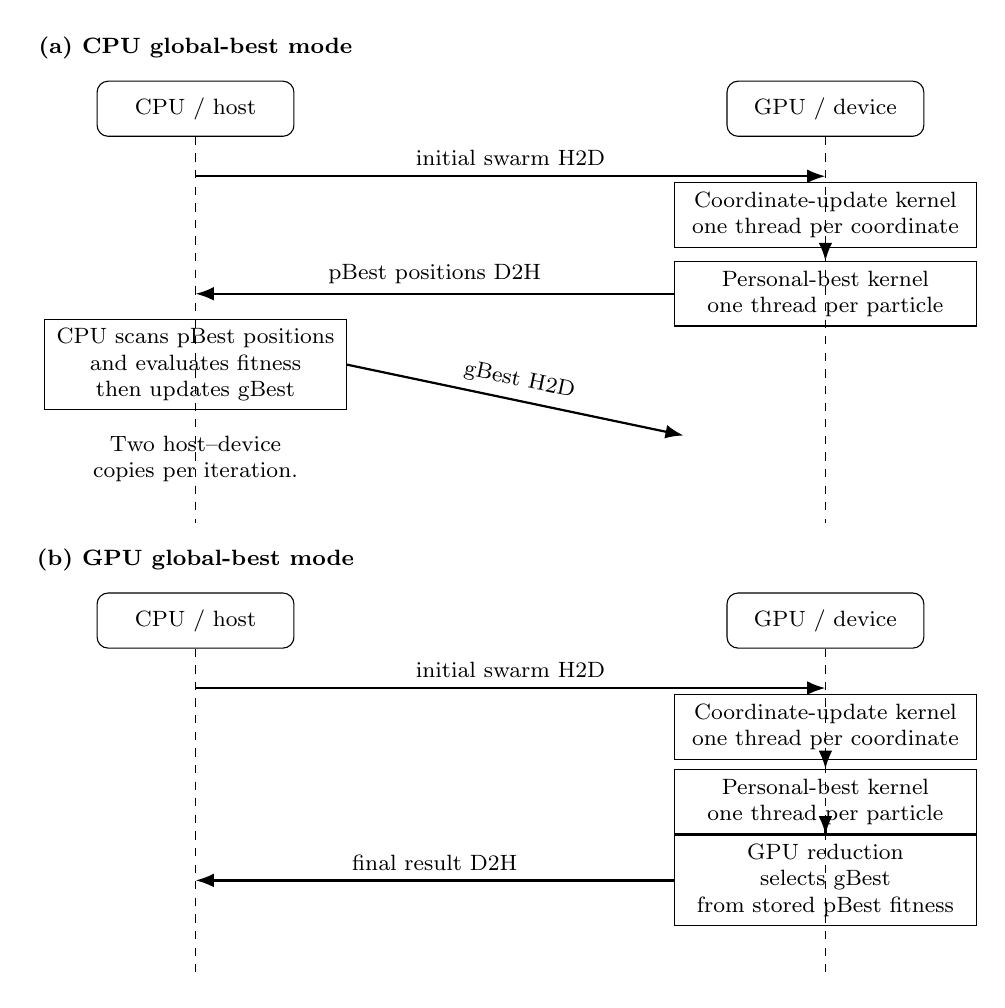
\begin{tikzpicture}[
  actor/.style={draw,rounded corners,align=center,minimum width=2.5cm,
                minimum height=0.7cm},
  note/.style={draw,align=center,text width=3.6cm,minimum height=0.65cm},
  flow/.style={-{Latex},thick},
  every node/.style={font=\footnotesize}
]
\node[actor] (cpu1) at (0,0) {CPU / host};
\node[actor] (gpu1) at (8,0) {GPU / device};
\node[above=0.15cm of cpu1] {\textbf{(a) CPU global-best mode}};
\draw[dashed] (cpu1.south) -- ++(0,-4.9);
\draw[dashed] (gpu1.south) -- ++(0,-4.9);
\draw[flow] ([yshift=-0.5cm]cpu1.south) --
  node[above,sloped]{initial swarm H2D} ([yshift=-0.5cm]gpu1.south);
\node[note] (coord1) at (8,-1.35)
  {Coordinate-update kernel\\one thread per coordinate};
\node[note] (pbest1) at (8,-2.35)
  {Personal-best kernel\\one thread per particle};
\draw[flow] (coord1) -- (pbest1);
\draw[flow] (pbest1.west) -- node[above]{pBest positions D2H} (0,-2.35);
\node[note] (scan) at (0,-3.25)
  {CPU scans pBest positions and evaluates fitness\\then updates gBest};
\draw[flow] (scan.east) --
  node[above,sloped]{gBest H2D} (6.2,-4.15);
\node[below=0.2cm of scan,align=center,text width=4.0cm]
  {Two host--device copies per iteration.};

\node[actor] (cpu2) at (0,-6.5) {CPU / host};
\node[actor] (gpu2) at (8,-6.5) {GPU / device};
\node[above=0.15cm of cpu2] {\textbf{(b) GPU global-best mode}};
\draw[dashed] (cpu2.south) -- ++(0,-4.2);
\draw[dashed] (gpu2.south) -- ++(0,-4.2);
\draw[flow] ([yshift=-0.5cm]cpu2.south) --
  node[above,sloped]{initial swarm H2D} ([yshift=-0.5cm]gpu2.south);
\node[note] (coord2) at (8,-7.85)
  {Coordinate-update kernel\\one thread per coordinate};
\node[note] (pbest2) at (8,-8.8)
  {Personal-best kernel\\one thread per particle};
\node[note] (reduce) at (8,-9.8)
  {GPU reduction selects gBest\\from stored pBest fitness};
\draw[flow] (coord2) -- (pbest2);
\draw[flow] (pbest2) -- (reduce);
\draw[flow] (reduce.west) -- node[above]{final result D2H} (0,-9.8);
\end{tikzpicture}
\caption{Host--device sequence for the two global-best modes. The corrected
GPU mode removes the per-iteration personal-best transfers.}
\label{fig:pso-sequence}
\end{figure*}

\begin{figure}[t]
\centering
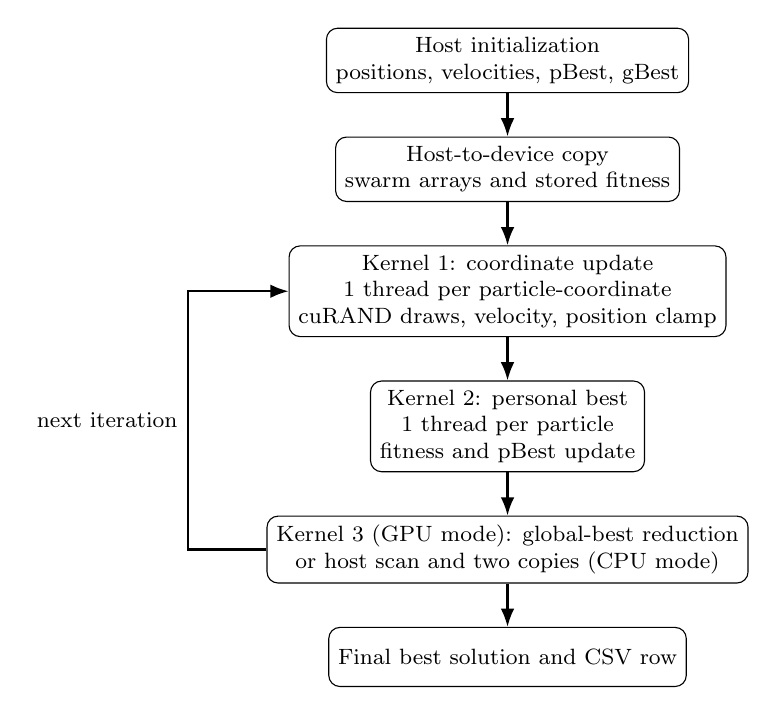
\begin{tikzpicture}[
  box/.style={draw,rounded corners,align=center,minimum width=3.3cm,
              minimum height=0.75cm},
  flow/.style={-{Latex},thick},
  every node/.style={font=\footnotesize}
]
\node[box] (init) {Host initialization\\positions, velocities, pBest, gBest};
\node[box,below=0.55cm of init] (transfer) {Host-to-device copy\\swarm arrays and stored fitness};
\node[box,below=0.55cm of transfer] (coord) {Kernel 1: coordinate update\\1 thread per particle-coordinate\\cuRAND draws, velocity, position clamp};
\node[box,below=0.55cm of coord] (pbest) {Kernel 2: personal best\\1 thread per particle\\fitness and pBest update};
\node[box,below=0.55cm of pbest] (select) {Kernel 3 (GPU mode): global-best reduction\\or host scan and two copies (CPU mode)};
\node[box,below=0.55cm of select] (result) {Final best solution and CSV row};
\draw[flow] (init) -- (transfer);
\draw[flow] (transfer) -- (coord);
\draw[flow] (coord) -- (pbest);
\draw[flow] (pbest) -- (select);
\draw[flow] (select.west) -- ++(-1.0,0) |- (coord.west)
  node[pos=0.25,left]{next iteration};
\draw[flow] (select) -- (result);
\end{tikzpicture}
\caption{Kernel and data-flow architecture of the corrected CUDA PSO.}
\label{fig:pso-kernels}
\end{figure}

\subsubsection{Corrections to the Instructor Code}
\label{sec:corrections}
Table~\ref{tab:corrections} summarizes the changes made to the supplied
program. They are intended to repair correctness and configurability while
preserving the PSO approach.

\begin{table*}[t]
\centering
\caption{Corrections and extensions to the instructor-provided PSO}
\label{tab:corrections}
\begin{tabular}{p{0.31\textwidth}p{0.62\textwidth}}
\toprule
\textbf{Problem in the supplied code} & \textbf{Correction in the current project}\\
\midrule
Dimension, population, and selected function were compile-time constants.
& Function, dimension, population, and number of runs are command-line inputs.\\
The loop used $n\,10^4$ iterations rather than an evaluation budget.
& Iterations are $\lfloor 10^4 n/N\rfloor$, corresponding to a maximum of
$10^4 n$ particle evaluations.\\
The objective selection included Levy and used incorrect/missing shift,
domain, or bias handling; Griewank's product began at zero.
& Four shifted objectives (Sphere, Rastrigin, Rosenbrock, Griewank) use their
specified domains and biases in the shared \texttt{benchmarks.h}; Levy is
removed and the Griewank product starts at one.\\
Global \texttt{\_\_device\_\_} temporary particle arrays were shared by threads.
& Per-particle temporary data is local to the fitness-evaluation thread; no
shared global scratch array is used.\\
$r_1$ and $r_2$ were drawn on the CPU once per iteration.
& cuRAND state is initialized per linear coordinate index; each update thread
draws fresh values for its particle-coordinate pair.\\
Personal-best fitness was recomputed when comparing candidates.
& One fitness value is stored per particle and updated together with its
personal-best position.\\
Block count was computed using floating-point ceiling on integer division.
& Grid sizes use integer ceiling division, $(s+t-1)/t$.\\
Position updates were not consistently restricted to the benchmark domain,
and CUDA errors were not checked.
& Updated positions are clamped to the domain, and kernel launches, device
synchronization, allocations, copies, and events are checked.\\
The global best was scanned on the CPU after two per-iteration transfers.
& Both this CPU mode (\texttt{--gbest cpu}) and a device reduction mode
(\texttt{--gbest gpu}) are available.\\
No sequential executable with the same benchmark interface was supplied.
& A sequential PSO uses the same objective header, parameter values,
initialization scheme, update logic, and evaluation budget.\\
\bottomrule
\end{tabular}
\end{table*}

\subsubsection{Improved PSO Variant}
\label{sec:pso-improved}
The base PSO uses $\omega=0.5$ and $c_1=c_2=1.5$, without a velocity bound.
At dimension 100 and population 100, the base method was observed to diverge
on Sphere in both the sequential and GPU implementations. The same behavior
on both implementations indicates that this particular failure is not
explained solely by GPU parallelization.

The improved variant retains the cognitive and social coefficients, the
initialization, the evaluation budget, and the position clamp. It changes
inertia according to
\begin{equation}
  \omega(t)=\omega_{\max}
  -(\omega_{\max}-\omega_{\min})\frac{t}{T-1},
  \quad \omega_{\max}=0.9,\quad \omega_{\min}=0.4,
\end{equation}
and clamps each velocity component to
\begin{equation}
  v_{i,j}(t+1)\leftarrow
  \min\!\left(v_{\max},\max(-v_{\max},v_{i,j}(t+1))\right),
  \qquad
  v_{\max}=\alpha(b_{\max}-b_{\min}).
\end{equation}
The current shared setting is $\alpha=0.1$. A trial value of $0.2$ did not
converge reliably on Sphere at dimension 100 over three runs, so $0.1$ was
retained. When $T=1$, the implementation uses the base inertia as a
well-defined fallback because the linear schedule denominator would be zero.

\section{Experimental Results}
\label{sec:results}
\subsection{Experimental Setup}
\label{sec:setup}
The reported GPU target is an NVIDIA T4 on Google Colab, compiled using
\texttt{nvcc}, CUDA 12, and \texttt{-arch=sm\_75}. The project provides a
sequential executable compiled with a C++17 compiler. The population sizes,
dimensions, number of independent runs, and GPU global-best mode are supplied
at runtime. Unless otherwise stated, each run receives a distinct seed.

The measurements in this section are preliminary project results supplied
for this article. The complete raw logs, exact Colab session metadata, and
confidence intervals are not currently included in the repository.
\todo{Archive raw CSV logs, record GPU/driver/compiler versions and seed
policy, and repeat all configurations before treating the measurements as
final.}

\subsection{Benchmark Functions}
\label{sec:benchmarks}
The shared header defines four shifted objective functions. The coordinate
indices below are one-based for mathematical readability. Let
$\mathbf{o}\in\R^n$ be the deterministic shift vector and define the
coordinate-wise shifted variables as indicated:
\begin{align}
 f_{\mathrm{Sphere}}(\mathbf{x})
 &= \sum_{i=1}^{n}(x_i-o_i)^2 - 450,
 && x_i\in[-100,100],\\
 f_{\mathrm{Rastrigin}}(\mathbf{x})
 &= \sum_{i=1}^{n}\left[z_i^2-10\cos(2\pi z_i)+10\right]-330,
 && z_i=x_i-o_i,\quad x_i\in[-5,5],\\
 f_{\mathrm{Rosenbrock}}(\mathbf{x})
 &= \sum_{i=1}^{n-1}
 \left[100(z_i^2-z_{i+1})^2+(z_i-1)^2\right]+390,
 && z_i=x_i-o_i+1,\quad x_i\in[-100,100],\\
 f_{\mathrm{Griewank}}(\mathbf{x})
 &= \sum_{i=1}^{n}\frac{(x_i-o_i)^2}{4000}
 -\prod_{i=1}^{n}\cos\!\left(\frac{x_i-o_i}{\sqrt{i}}\right)+1-180,
 && x_i\in[-600,600].
\end{align}
The shift is reproducible and generated coordinate-wise by the code as
\begin{equation}
 q_i=((((i-1)\bmod 101)\cdot37+17)\bmod101),\qquad
 o_i=\left(\frac{q_i}{100}-\frac{1}{2}\right)
       0.2(b_{\max}-b_{\min}).
\end{equation}
This is the project's deterministic shift construction; it should not be
mistaken for an externally supplied CEC shift vector. At $\mathbf{x}=\mathbf{o}$,
the four benchmark expressions evaluate to their respective biases
$-450,-330,390,-180$. The project reports that this consistency check passed
on both CPU and GPU. The GPU check evaluates the shared header's objective
on device for a ten-dimensional shift point. These are benchmark function
families used in real-parameter optimization studies
\cite{suganthan2005cec}; this project's particular shifts, domains, and
biases are custom settings and do not by themselves establish compliance
with the CEC 2005 benchmark definitions.

\subsection{Preliminary Results}
\label{sec:preliminary}
Table~\ref{tab:seq-preliminary} gives the supplied mean best fitness from
three sequential runs. The settings are population 50 at dimension 10 and
population 100 at dimension 100. These values are preliminary and are not
accompanied by standard deviations.

\begin{table}[t]
\centering
\caption{Preliminary sequential mean minima over three runs}
\label{tab:seq-preliminary}
\begin{tabular}{clrr}
\toprule
\textbf{Dim.} & \textbf{Function} & \textbf{Base} & \textbf{Improved}\\
\midrule
10 & Sphere     & -450.000 & -450.000\\
10 & Rastrigin  & -315.739 & -325.025\\
10 & Rosenbrock & 7273.664 & 390.191\\
10 & Griewank   & -179.923 & -179.912\\
\midrule
100 & Sphere     & 38437.802 & -449.995\\
100 & Rastrigin  & 388.690 & -142.948\\
100 & Rosenbrock & 8724032176.667 & 718.089\\
100 & Griewank   & 193.794 & -179.999\\
\bottomrule
\end{tabular}
\end{table}

For Sphere at dimension 100, the improved sequential mean is within
approximately $0.005$ of the bias, whereas the base mean is far from the
optimum. The improved method also substantially lowers the reported
Rosenbrock values, but its dimension-100 result remains above the bias.
Rastrigin and Rosenbrock remain difficult at dimension 100 for this PSO
configuration. The shift and bias do not change the underlying search
difficulty.

Table~\ref{tab:de-sequential-preliminary} summarizes the three-run sequential
DE campaign executed for this project. Each entry is the mean best fitness;
raw run-level CSV files and standard deviations were not retained. The
default DE/rand/1/bin results at dimension 100 are at least as good as the
reported improved-PSO means for Sphere, Rastrigin, and Rosenbrock. The other
strategies show that performance is strategy- and objective-dependent; these
small preliminary samples are not a statistical comparison.
\begin{table*}[t]
\centering
\caption{Preliminary sequential DE mean minima over three runs}
\label{tab:de-sequential-preliminary}
\begin{tabular}{clrrr}
\toprule
\textbf{Dim.} & \textbf{Function} & \textbf{rand/1/bin} &
\textbf{best/1/bin} & \textbf{current-to-best/1/bin}\\
\midrule
10 & Sphere     & -450.000 & -439.611 & -449.992\\
10 & Rastrigin  & -327.659 & -311.410 & -327.015\\
10 & Rosenbrock & 392.104 & 97752.484 & 3184.123\\
10 & Griewank   & -179.984 & -179.579 & -179.890\\
\midrule
100 & Sphere     & -450.000 & 49029.773 & 25466.590\\
100 & Rastrigin  & -147.364 & 275.673 & -31.510\\
100 & Rosenbrock & 538.030 & $5.508\times10^9$ & $1.775\times10^9$\\
100 & Griewank   & -179.997 & 361.173 & 37.693\\
\bottomrule
\end{tabular}
\end{table*}

The supplied three-run GPU measurements for the improved variant at
dimension 100 and population 100 are summarized in
Table~\ref{tab:gpu-preliminary}. The Rosenbrock values are reported
individually because no mean or dispersion was supplied.
\begin{table}[t]
\centering
\caption{Preliminary GPU improved-variant results, $n=100$, $N=100$}
\label{tab:gpu-preliminary}
\begin{tabular}{lc}
\toprule
\textbf{Function} & \textbf{Reported best fitness}\\
\midrule
Sphere & $-449.9999$ (error approximately $10^{-4}$)\\
Rosenbrock & $452.7,\ 638.5,\ 623.2$\\
Griewank & $-179.9999$\\
\bottomrule
\end{tabular}
\end{table}
\todo{Add the missing GPU Rastrigin results and raw run-level CSV values.}

\subsection{Runtime and Planned Full Campaign}
\label{sec:campaign}
Table~\ref{tab:timings} records preliminary per-run timings supplied for the
project. They are not a complete controlled benchmark campaign.
\begin{table}[t]
\centering
\caption{Supplied preliminary base-PSO runtime measurements}
\label{tab:timings}
\begin{tabular}{lllr}
\toprule
\textbf{Dim.} & \textbf{Population / function} &
\textbf{Configuration} & \textbf{Time}\\
\midrule
10 & 50 / Griewank & GPU, CPU gBest & $\sim0.08$ s\\
10 & 50 / Griewank & GPU, GPU gBest & $\sim0.06$ s\\
10 & 500 / Sphere & GPU, CPU gBest & $\sim0.011$ s\\
10 & 500 / Sphere & GPU, GPU gBest & $\sim0.006$ s\\
100 & 100 / Sphere & Sequential & $\sim3.5$ s\\
100 & 100 / Sphere & GPU, CPU gBest & $\sim1.0$ s\\
100 & 100 / Sphere & GPU, GPU gBest & $\sim0.34$ s\\
50 & 100 / TODO: function & Sequential & $\sim0.89$ s\\
50 & 100 / TODO: function & GPU & $\sim0.15$ s\\
\bottomrule
\end{tabular}
\end{table}
For the dimension-100 Sphere case, the reported sequential-to-GPU ratio is
approximately $3.5/0.34\simeq10.3$. The GPU global-best reduction is faster
in the supplied examples than the CPU scan mode; a plausible explanation is
that it removes repeated host--device transfers of the personal-best array
and global-best vector. This interpretation should be confirmed with
controlled repetitions and profiling. The original instructor program,
using Levy, dimension 3, 512 particles, and 30,000 iterations, reportedly
took 10.4 s. This is a historical baseline with a different objective and
workload and is not directly comparable to the corrected experiments.

The complete ten-run campaign summaries and statistical tests are generated
from the run-level CSV files and included in Section~\ref{sec:generated-analysis}.
The reported tests use an unadjusted nominal significance threshold; effect
sizes and corrections for multiple comparisons remain a subject for further
analysis.

\subsection{Comparison with the Literature}
\label{sec:literature}
\todo{After target-GPU validation, compare the CUDA DE implementation and
measured workload with
\emph{An Improved CUDA-Based Implementation of Differential Evolution}.
Verify the bibliographic record and ensure that hardware, objective
definitions, evaluation budgets, and timing boundaries are comparable before
making quantitative claims.}

\subsection{Generated Campaign Analysis}
\label{sec:generated-analysis}
The campaign analysis script reads only CSV files under
\texttt{results/}; incomplete inputs are reported and missing groups are
omitted rather than imputed. The generated summary tables report the mean and
sample standard deviation of both minimum fitness and error from the known
benchmark bias. Timing summaries and sequential-to-GPU speedups are reported
separately. The figures show runtime versus dimension by population,
speedup versus population, and representative minimum-fitness box plots.
Statistical comparisons use the two-sided Mann--Whitney rank-sum test for
independent runs with different seeds, and Kruskal--Wallis for the three DE
strategies. An ``='' entry marks samples that are all identical, for which a
test is not meaningful. A nominal significance threshold of 0.05 is used
without a multiple-comparison correction. Rapid-run or missing-file outputs
are exploratory and are not a substitute for the full ten-run campaign.

\paragraph{GPU comparison at Pop=100}
Table~\ref{tab:pso-vs-de-gpu-pop100} compares the improved PSO with GPU
global-best reduction against DE/rand/1 on the same function, dimension, and
population. The quality label selects an algorithm only when the existing
two-sided Mann--Whitney test is significant at $p<0.05$ and its sample mean
minimum is lower; a non-significant result is reported as no significant
difference. Runtime ratios and descriptive statistics are computed directly
from the corresponding run-level CSV rows.

\begin{table*}[t]
\centering
\caption{Comparaison GPU PSO ameliore et DE rand1, Pop=100}
\label{tab:pso-vs-de-gpu-pop100}
\scriptsize
\begin{tabular}{lllllll}
\toprule
Fonction & Dim. & PSO améliore (moy. ± ET; méd.; s) & DE rand1 (moy. ± ET; méd.; s) & Temps DE / PSO & p Mann–Whitney & Meilleur qualité \\
\midrule
1 & 10 & -450 $\pm$ 0; -450; 0.02249 & -450 $\pm$ 0; -450; 0.01117 & 0.4968 & = & Identiques (=) \\
1 & 50 & -450 $\pm$ 1.58e-05; -450; 0.1385 & -450 $\pm$ 0; -450; 0.1521 & 1.098 & 4.731e-05 & DE rand1 GPU \\
1 & 100 & -450 $\pm$ 0.000411; -450; 0.3366 & -450 $\pm$ 1.6e-05; -450; 0.5776 & 1.716 & 0.0001247 & DE rand1 GPU \\
2 & 10 & -325.22 $\pm$ 2.43; -325.52; 0.0232 & -310.71 $\pm$ 2.65; -310.98; 0.01171 & 0.5046 & 0.0001766 & PSO ameliore GPU \\
2 & 50 & -248.59 $\pm$ 18.7; -253.89; 0.1703 & -92.218 $\pm$ 57.7; -85.44; 0.1776 & 1.043 & 0.0001827 & PSO ameliore GPU \\
2 & 100 & -116.69 $\pm$ 42.4; -124.04; 0.4622 & -246.41 $\pm$ 65; -266.32; 0.6833 & 1.478 & 0.002202 & DE rand1 GPU \\
3 & 10 & 400.68 $\pm$ 27.5; 391.47; 0.02187 & 390 $\pm$ 0.00054; 390; 0.01148 & 0.5252 & 0.0001212 & DE rand1 GPU \\
3 & 50 & 70680 $\pm$ 2.22e+05; 480.08; 0.1587 & 424.9 $\pm$ 22.9; 414.47; 0.1633 & 1.029 & 0.01402 & DE rand1 GPU \\
3 & 100 & 94961 $\pm$ 2.95e+05; 590.18; 0.4218 & 506.65 $\pm$ 31.6; 515.32; 0.6302 & 1.494 & 0.0002461 & DE rand1 GPU \\
4 & 10 & -179.94 $\pm$ 0.0227; -179.94; 0.0238 & -179.78 $\pm$ 0.101; -179.78; 0.013 & 0.5461 & 0.002827 & PSO ameliore GPU \\
4 & 50 & -179.99 $\pm$ 0.0103; -179.99; 0.1938 & -180 $\pm$ 0; -180; 0.2038 & 1.052 & 6.113e-05 & DE rand1 GPU \\
4 & 100 & -179.99 $\pm$ 0.0118; -180; 0.562 & -180 $\pm$ 0.00734; -180; 0.7933 & 1.411 & 0.01327 & DE rand1 GPU \\
\bottomrule
\end{tabular}
\end{table*}


\begin{figure*}[t]
\centering
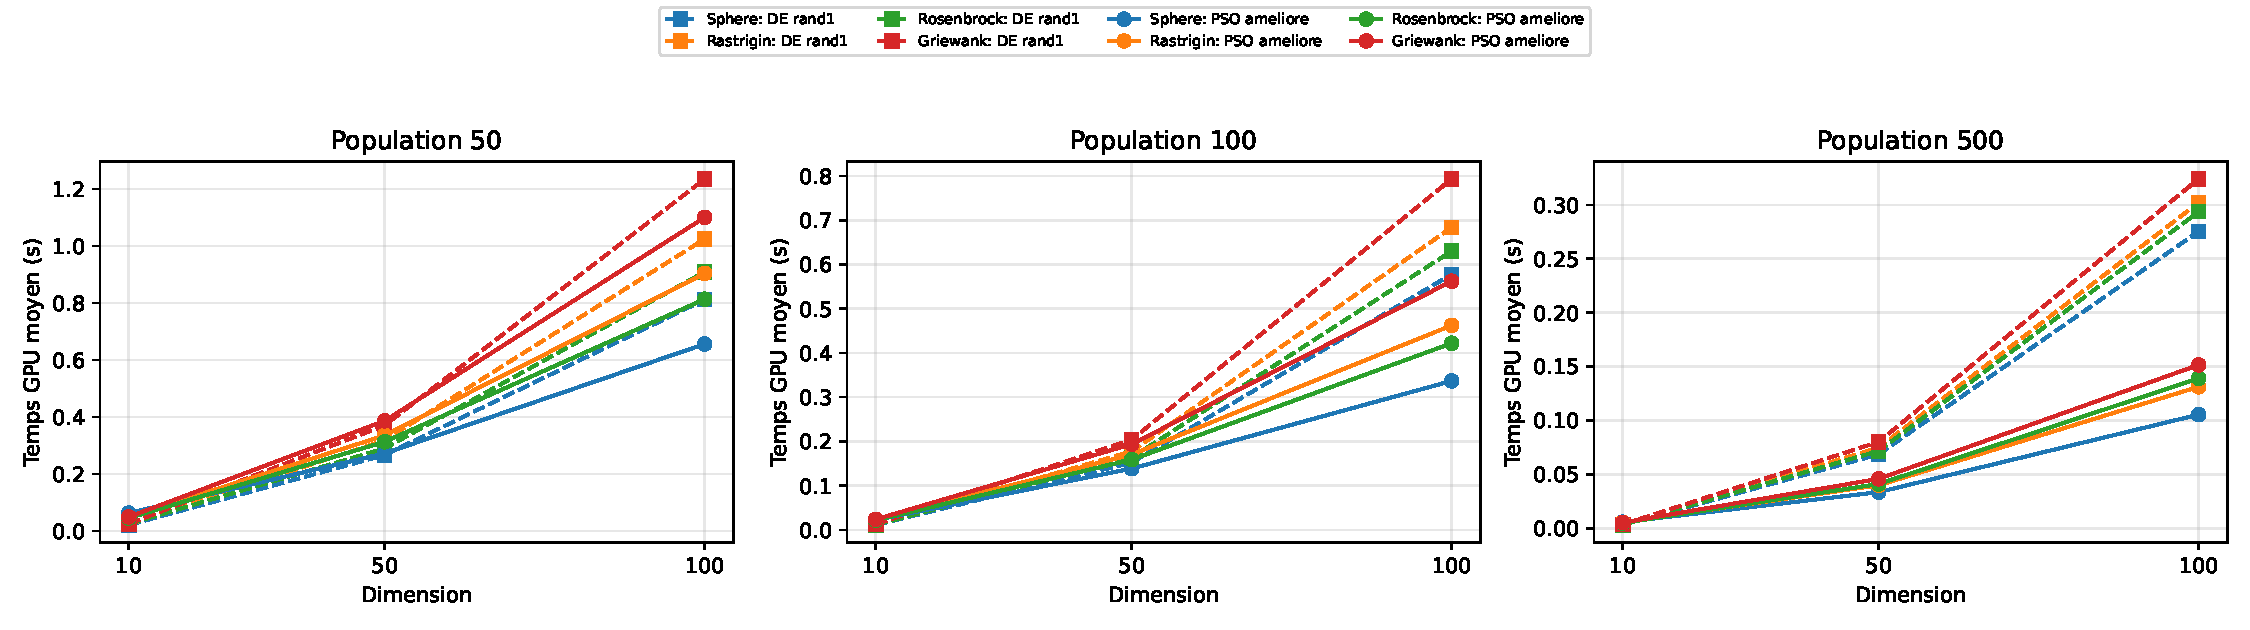
\includegraphics[width=\textwidth]{figures/pso_vs_de_gpu_runtime.pdf}
\caption{Measured GPU runtime for improved PSO with GPU global-best
reduction and DE/rand/1 as a function of dimension, separated by population
and benchmark function.}
\label{fig:pso-vs-de-gpu-runtime}
\end{figure*}

\begin{table*}[t]
\centering
\caption{Moyenne et ecart-type des minima et des erreurs aux biais}
\label{tab:generated-minima}
\scriptsize
\begin{tabular}{llllllllllll}
\toprule
algo & version & fonction & dim & pop & runs & minimum\_mean & minimum\_std & error\_mean & error\_std & minimum\_mean\_pm\_std & error\_mean\_pm\_std \\
\midrule
de-best1 & gpu & 1 & 10 & 50 & 10 & -443.78887640000005 & 8.355905136525234 & 6.2111236576312 & 8.355905256118982 & -443.789 $\pm$ 8.356 & 6.21112 $\pm$ 8.356 \\
de-best1 & seq & 1 & 10 & 50 & 10 & -437.59020380000004 & 23.283792435546594 & 12.409796136721999 & 23.283792323222027 & -437.59 $\pm$ 23.28 & 12.4098 $\pm$ 23.28 \\
de-currenttobest1 & gpu & 1 & 10 & 50 & 10 & -449.97471299999995 & 0.056056148737968964 & 0.02528686523643 & 0.05605631779092117 & -449.975 $\pm$ 0.05606 & 0.0252869 $\pm$ 0.05606 \\
de-currenttobest1 & seq & 1 & 10 & 50 & 10 & -449.43694450000004 & 1.7643057755033789 & 0.5630554201193799 & 1.764305804951932 & -449.437 $\pm$ 1.764 & 0.563055 $\pm$ 1.764 \\
de-rand1 & gpu & 1 & 10 & 50 & 10 & -450.0 & 0.0 & 0.0 & 0.0 & -450 $\pm$ 0 & 0 $\pm$ 0 \\
de-rand1 & seq & 1 & 10 & 50 & 10 & -450.0 & 0.0 & 0.0 & 0.0 & -450 $\pm$ 0 & 0 $\pm$ 0 \\
pso & gpu-gbest-gpu & 1 & 10 & 50 & 10 & -450.0 & 0.0 & 0.0 & 0.0 & -450 $\pm$ 0 & 0 $\pm$ 0 \\
pso & seq & 1 & 10 & 50 & 10 & -449.99999690000004 & 9.80306074666226e-06 & 3.05175781e-06 & 9.650505546807378e-06 & -450 $\pm$ 9.803e-06 & 3.05176e-06 $\pm$ 9.651e-06 \\
pso-ameliore & gpu-gbest-gpu & 1 & 10 & 50 & 10 & -450.0 & 0.0 & 0.0 & 0.0 & -450 $\pm$ 0 & 0 $\pm$ 0 \\
pso-ameliore & seq & 1 & 10 & 50 & 10 & -450.0 & 0.0 & 0.0 & 0.0 & -450 $\pm$ 0 & 0 $\pm$ 0 \\
de-best1 & gpu & 1 & 10 & 100 & 10 & -449.99998450000004 & 1.6338434576721338e-05 & 1.525878905e-05 & 1.608417591134563e-05 & -450 $\pm$ 1.634e-05 & 1.52588e-05 $\pm$ 1.608e-05 \\
de-best1 & seq & 1 & 10 & 100 & 10 & -449.9999815 & 2.1454085330221128e-05 & 1.8310546859999998e-05 & 2.133807062400243e-05 & -450 $\pm$ 2.145e-05 & 1.83105e-05 $\pm$ 2.134e-05 \\
de-currenttobest1 & gpu & 1 & 10 & 100 & 10 & -450.0 & 0.0 & 0.0 & 0.0 & -450 $\pm$ 0 & 0 $\pm$ 0 \\
de-currenttobest1 & seq & 1 & 10 & 100 & 10 & -450.0 & 0.0 & 0.0 & 0.0 & -450 $\pm$ 0 & 0 $\pm$ 0 \\
de-rand1 & gpu & 1 & 10 & 100 & 10 & -450.0 & 0.0 & 0.0 & 0.0 & -450 $\pm$ 0 & 0 $\pm$ 0 \\
de-rand1 & seq & 1 & 10 & 100 & 10 & -450.0 & 0.0 & 0.0 & 0.0 & -450 $\pm$ 0 & 0 $\pm$ 0 \\
pso & gpu-gbest-gpu & 1 & 10 & 100 & 10 & -450.0 & 0.0 & 0.0 & 0.0 & -450 $\pm$ 0 & 0 $\pm$ 0 \\
pso & seq & 1 & 10 & 100 & 10 & -450.0 & 0.0 & 0.0 & 0.0 & -450 $\pm$ 0 & 0 $\pm$ 0 \\
pso-ameliore & gpu-gbest-gpu & 1 & 10 & 100 & 10 & -450.0 & 0.0 & 0.0 & 0.0 & -450 $\pm$ 0 & 0 $\pm$ 0 \\
pso-ameliore & seq & 1 & 10 & 100 & 10 & -450.0 & 0.0 & 0.0 & 0.0 & -450 $\pm$ 0 & 0 $\pm$ 0 \\
de-best1 & gpu & 1 & 10 & 500 & 10 & -450.0 & 0.0 & 0.0 & 0.0 & -450 $\pm$ 0 & 0 $\pm$ 0 \\
de-best1 & seq & 1 & 10 & 500 & 10 & -450.0 & 0.0 & 0.0 & 0.0 & -450 $\pm$ 0 & 0 $\pm$ 0 \\
de-currenttobest1 & gpu & 1 & 10 & 500 & 10 & -450.0 & 0.0 & 0.0 & 0.0 & -450 $\pm$ 0 & 0 $\pm$ 0 \\
de-currenttobest1 & seq & 1 & 10 & 500 & 10 & -450.0 & 0.0 & 0.0 & 0.0 & -450 $\pm$ 0 & 0 $\pm$ 0 \\
de-rand1 & gpu & 1 & 10 & 500 & 10 & -449.9997311999999 & 7.144974923917117e-05 & 0.0002685546875 & 7.164232116710267e-05 & -450 $\pm$ 7.145e-05 & 0.000268555 $\pm$ 7.164e-05 \\
de-rand1 & seq & 1 & 10 & 500 & 10 & -449.99976180000004 & 8.496116759479361e-05 & 0.00023803710932 & 8.48659406524553e-05 & -450 $\pm$ 8.496e-05 & 0.000238037 $\pm$ 8.487e-05 \\
pso & gpu-gbest-gpu & 1 & 10 & 500 & 10 & -450.0 & 0.0 & 0.0 & 0.0 & -450 $\pm$ 0 & 0 $\pm$ 0 \\
pso & seq & 1 & 10 & 500 & 10 & -450.0 & 0.0 & 0.0 & 0.0 & -450 $\pm$ 0 & 0 $\pm$ 0 \\
pso-ameliore & gpu-gbest-gpu & 1 & 10 & 500 & 10 & -450.0 & 0.0 & 0.0 & 0.0 & -450 $\pm$ 0 & 0 $\pm$ 0 \\
pso-ameliore & seq & 1 & 10 & 500 & 10 & -450.0 & 0.0 & 0.0 & 0.0 & -450 $\pm$ 0 & 0 $\pm$ 0 \\
de-best1 & gpu & 1 & 50 & 50 & 10 & 14052.55117 & 3187.229788189667 & 14502.55117 & 3187.229788189667 & 14052.6 $\pm$ 3187 & 14502.6 $\pm$ 3187 \\
de-best1 & seq & 1 & 50 & 50 & 10 & 16879.02481 & 4109.048459418863 & 17329.02481 & 4109.048459418863 & 16879 $\pm$ 4109 & 17329 $\pm$ 4109 \\
de-currenttobest1 & gpu & 1 & 50 & 50 & 10 & 7082.210206000001 & 1542.5571895654587 & 7532.210206000001 & 1542.5571895654587 & 7082.21 $\pm$ 1543 & 7532.21 $\pm$ 1543 \\
de-currenttobest1 & seq & 1 & 50 & 50 & 10 & 8594.336621 & 2128.1736195617113 & 9044.336620999999 & 2128.1736195617113 & 8594.34 $\pm$ 2128 & 9044.34 $\pm$ 2128 \\
de-rand1 & gpu & 1 & 50 & 50 & 10 & -450.0 & 0.0 & 0.0 & 0.0 & -450 $\pm$ 0 & 0 $\pm$ 0 \\
de-rand1 & seq & 1 & 50 & 50 & 10 & -450.0 & 0.0 & 0.0 & 0.0 & -450 $\pm$ 0 & 0 $\pm$ 0 \\
pso & gpu-gbest-gpu & 1 & 50 & 50 & 10 & 4537.289991 & 2002.205332097175 & 4987.289995 & 2002.205343735581 & 4537.29 $\pm$ 2002 & 4987.29 $\pm$ 2002 \\
pso & seq & 1 & 50 & 50 & 10 & 7544.226390000001 & 4099.270800096661 & 7994.226381999999 & 4099.270795380034 & 7544.23 $\pm$ 4099 & 7994.23 $\pm$ 4099 \\
pso-ameliore & gpu-gbest-gpu & 1 & 50 & 50 & 10 & -449.999957 & 1.5491933399657816e-05 & 4.272460934e-05 & 1.5759209566384556e-05 & -450 $\pm$ 1.549e-05 & 4.27246e-05 $\pm$ 1.576e-05 \\
pso-ameliore & seq & 1 & 50 & 50 & 10 & -449.99992970000005 & 1.4974422628882377e-05 & 7.019042965999999e-05 & 1.474139076924992e-05 & -450 $\pm$ 1.497e-05 & 7.01904e-05 $\pm$ 1.474e-05 \\
de-best1 & gpu & 1 & 50 & 100 & 10 & 10822.659084 & 2640.2252979571504 & 11272.659084 & 2640.2252979571504 & 10822.7 $\pm$ 2640 & 11272.7 $\pm$ 2640 \\
de-best1 & seq & 1 & 50 & 100 & 10 & 10928.23091 & 3424.0553538949766 & 11378.230911 & 3424.0553534653004 & 10928.2 $\pm$ 3424 & 11378.2 $\pm$ 3424 \\
de-currenttobest1 & gpu & 1 & 50 & 100 & 10 & 3368.627319 & 1387.379896985601 & 3818.627319 & 1387.379896985601 & 3368.63 $\pm$ 1387 & 3818.63 $\pm$ 1387 \\
de-currenttobest1 & seq & 1 & 50 & 100 & 10 & 3811.482079 & 988.2326315860768 & 4261.482078999999 & 988.2326315860768 & 3811.48 $\pm$ 988.2 & 4261.48 $\pm$ 988.2 \\
de-rand1 & gpu & 1 & 50 & 100 & 10 & -450.0 & 0.0 & 0.0 & 0.0 & -450 $\pm$ 0 & 0 $\pm$ 0 \\
de-rand1 & seq & 1 & 50 & 100 & 10 & -450.0 & 0.0 & 0.0 & 0.0 & -450 $\pm$ 0 & 0 $\pm$ 0 \\
pso & gpu-gbest-gpu & 1 & 50 & 100 & 10 & 4240.552952 & 2945.477820116541 & 4690.552952 & 2945.477820116541 & 4240.55 $\pm$ 2945 & 4690.55 $\pm$ 2945 \\
pso & seq & 1 & 50 & 100 & 10 & 5404.2903886 & 4591.798540843569 & 5854.290389 & 4591.79854039296 & 5404.29 $\pm$ 4592 & 5854.29 $\pm$ 4592 \\
pso-ameliore & gpu-gbest-gpu & 1 & 50 & 100 & 10 & -449.999954 & 1.5811388315704354e-05 & 4.577636715e-05 & 1.6084175911345627e-05 & -450 $\pm$ 1.581e-05 & 4.57764e-05 $\pm$ 1.608e-05 \\
pso-ameliore & seq & 1 & 50 & 100 & 10 & -449.99992970000005 & 1.4974422634805146e-05 & 7.019042965999999e-05 & 1.4741390769249925e-05 & -450 $\pm$ 1.497e-05 & 7.01904e-05 $\pm$ 1.474e-05 \\
de-best1 & gpu & 1 & 50 & 500 & 10 & 2545.128957 & 860.1345393019648 & 2995.128957 & 860.1345393019649 & 2545.13 $\pm$ 860.1 & 2995.13 $\pm$ 860.1 \\
de-best1 & seq & 1 & 50 & 500 & 10 & 2378.5247200000003 & 764.2002035217423 & 2828.5247200000003 & 764.2002035217423 & 2378.52 $\pm$ 764.2 & 2828.52 $\pm$ 764.2 \\
de-currenttobest1 & gpu & 1 & 50 & 500 & 10 & -265.55442822 & 115.11148966924345 & 184.44557181 & 115.11148970362466 & -265.554 $\pm$ 115.1 & 184.446 $\pm$ 115.1 \\
de-currenttobest1 & seq & 1 & 50 & 500 & 10 & -233.3166855 & 140.7099272825963 & 216.68331447 & 140.7099273253592 & -233.317 $\pm$ 140.7 & 216.683 $\pm$ 140.7 \\
de-rand1 & gpu & 1 & 50 & 500 & 10 & -387.0521972 & 14.079190510286216 & 62.94780273 & 14.079190501363009 & -387.052 $\pm$ 14.08 & 62.9478 $\pm$ 14.08 \\
de-rand1 & seq & 1 & 50 & 500 & 10 & -385.23218080000004 & 14.908064619431471 & 64.76781921 & 14.90806453732183 & -385.232 $\pm$ 14.91 & 64.7678 $\pm$ 14.91 \\
pso & gpu-gbest-gpu & 1 & 50 & 500 & 10 & -223.3744385 & 147.24397358131037 & 226.62556152000002 & 147.24397356075087 & -223.374 $\pm$ 147.2 & 226.626 $\pm$ 147.2 \\
pso & seq & 1 & 50 & 500 & 10 & -298.14126736 & 132.01532624118477 & 151.8587326 & 132.0153261541061 & -298.141 $\pm$ 132 & 151.859 $\pm$ 132 \\
pso-ameliore & gpu-gbest-gpu & 1 & 50 & 500 & 10 & -449.99995090000004 & 2.1199842792965294e-05 & 4.882812496999999e-05 & 2.1338070646249885e-05 & -450 $\pm$ 2.12e-05 & 4.88281e-05 $\pm$ 2.134e-05 \\
pso-ameliore & seq & 1 & 50 & 500 & 10 & -449.9999235 & 1.63384345302966e-05 & 7.629394529999999e-05 & 1.6084175964050257e-05 & -450 $\pm$ 1.634e-05 & 7.62939e-05 $\pm$ 1.608e-05 \\
de-best1 & gpu & 1 & 100 & 50 & 10 & 58683.50272999999 & 10122.072978712029 & 59133.50272999999 & 10122.072978712029 & 58683.5 $\pm$ 1.012e+04 & 59133.5 $\pm$ 1.012e+04 \\
de-best1 & seq & 1 & 100 & 50 & 10 & 64225.20977 & 9896.15594739597 & 64675.20977 & 9896.15594739597 & 64225.2 $\pm$ 9896 & 64675.2 $\pm$ 9896 \\
de-currenttobest1 & gpu & 1 & 100 & 50 & 10 & 35248.34982 & 7266.701774284676 & 35698.34982 & 7266.701774284676 & 35248.3 $\pm$ 7267 & 35698.3 $\pm$ 7267 \\
de-currenttobest1 & seq & 1 & 100 & 50 & 10 & 33530.30294 & 8482.356915238823 & 33980.30294 & 8482.356915238823 & 33530.3 $\pm$ 8482 & 33980.3 $\pm$ 8482 \\
de-rand1 & gpu & 1 & 100 & 50 & 10 & -449.9999907 & 1.4974422625590222e-05 & 9.155273429999999e-06 & 1.4741390720945336e-05 & -450 $\pm$ 1.497e-05 & 9.15527e-06 $\pm$ 1.474e-05 \\
de-rand1 & seq & 1 & 100 & 50 & 10 & -449.9999752 & 1.3070747646564427e-05 & 2.441406248e-05 & 1.2867340729076503e-05 & -450 $\pm$ 1.307e-05 & 2.44141e-05 $\pm$ 1.287e-05 \\
pso & gpu-gbest-gpu & 1 & 100 & 50 & 10 & 63163.878119999994 & 13867.339487136813 & 63613.878119999994 & 13867.339487136813 & 63163.9 $\pm$ 1.387e+04 & 63613.9 $\pm$ 1.387e+04 \\
pso & seq & 1 & 100 & 50 & 10 & 61699.34611 & 13652.756363919196 & 62149.34611 & 13652.756363919196 & 61699.3 $\pm$ 1.365e+04 & 62149.3 $\pm$ 1.365e+04 \\
pso-ameliore & gpu-gbest-gpu & 1 & 100 & 50 & 10 & -449.99971910000005 & 0.00024291857345526237 & 0.00028076171878 & 0.0002432063556832676 & -450 $\pm$ 0.0002429 & 0.000280762 $\pm$ 0.0002432 \\
pso-ameliore & seq & 1 & 100 & 50 & 10 & -449.99314269999996 & 0.014535517848430915 & 0.006857299807899999 & 0.014535717847331467 & -449.993 $\pm$ 0.01454 & 0.0068573 $\pm$ 0.01454 \\
de-best1 & gpu & 1 & 100 & 100 & 10 & 44623.7039 & 5832.684864425106 & 45073.7039 & 5832.684864425106 & 44623.7 $\pm$ 5833 & 45073.7 $\pm$ 5833 \\
de-best1 & seq & 1 & 100 & 100 & 10 & 44465.12694 & 3612.149951847493 & 44915.12694 & 3612.149951847493 & 44465.1 $\pm$ 3612 & 44915.1 $\pm$ 3612 \\
de-currenttobest1 & gpu & 1 & 100 & 100 & 10 & 23969.44296 & 5025.309301535196 & 24419.44296 & 5025.309301535196 & 23969.4 $\pm$ 5025 & 24419.4 $\pm$ 5025 \\
de-currenttobest1 & seq & 1 & 100 & 100 & 10 & 24268.342979999998 & 3280.3071740038804 & 24718.342979999998 & 3280.3071740038804 & 24268.3 $\pm$ 3280 & 24718.3 $\pm$ 3280 \\
de-rand1 & gpu & 1 & 100 & 100 & 10 & -449.9999876 & 1.6008331146715744e-05 & 1.220703124e-05 & 1.5759209566384556e-05 & -450 $\pm$ 1.601e-05 & 1.2207e-05 $\pm$ 1.576e-05 \\
de-rand1 & seq & 1 & 100 & 100 & 10 & -449.99999379999997 & 1.3070747654666465e-05 & 6.10351562e-06 & 1.2867340729076503e-05 & -450 $\pm$ 1.307e-05 & 6.10352e-06 $\pm$ 1.287e-05 \\
pso & gpu-gbest-cpu & 1 & 100 & 100 & 10 & 46392.316399999996 & 8422.427739720117 & 46842.316399999996 & 8422.427739720117 & 46392.3 $\pm$ 8422 & 46842.3 $\pm$ 8422 \\
pso & gpu-gbest-gpu & 1 & 100 & 100 & 10 & 44126.82384 & 5889.580141923677 & 44576.82384 & 5889.580141923677 & 44126.8 $\pm$ 5890 & 44576.8 $\pm$ 5890 \\
pso & seq & 1 & 100 & 100 & 10 & 43350.34159 & 7009.6502966992775 & 43800.34159 & 7009.6502966992775 & 43350.3 $\pm$ 7010 & 43800.3 $\pm$ 7010 \\
pso-ameliore & gpu-gbest-cpu & 1 & 100 & 100 & 10 & -449.9990812 & 0.0014945449549047484 & 0.0009185791009999999 & 0.0014945964615134567 & -449.999 $\pm$ 0.001495 & 0.000918579 $\pm$ 0.001495 \\
pso-ameliore & gpu-gbest-gpu & 1 & 100 & 100 & 10 & -449.99973140000003 & 0.00041102506006700305 & 0.00026855468714 & 0.0004111513041448829 & -450 $\pm$ 0.000411 & 0.000268555 $\pm$ 0.0004112 \\
pso-ameliore & seq & 1 & 100 & 100 & 10 & -449.99844659999997 & 0.0030503101554428405 & 0.0015533447229000002 & 0.0030502807316305303 & -449.998 $\pm$ 0.00305 & 0.00155334 $\pm$ 0.00305 \\
de-best1 & gpu & 1 & 100 & 500 & 10 & 24728.843549999998 & 3193.1187172427794 & 25178.843549999998 & 3193.1187172427794 & 24728.8 $\pm$ 3193 & 25178.8 $\pm$ 3193 \\
de-best1 & seq & 1 & 100 & 500 & 10 & 25092.9332 & 3292.5935705320435 & 25542.9332 & 3292.5935705320435 & 25092.9 $\pm$ 3293 & 25542.9 $\pm$ 3293 \\
de-currenttobest1 & gpu & 1 & 100 & 500 & 10 & 8457.088959 & 2351.981802755776 & 8907.088958 & 2351.9818021567485 & 8457.09 $\pm$ 2352 & 8907.09 $\pm$ 2352 \\
de-currenttobest1 & seq & 1 & 100 & 500 & 10 & 7115.254248 & 1343.636092874095 & 7565.2542490000005 & 1343.6360951544336 & 7115.25 $\pm$ 1344 & 7565.25 $\pm$ 1344 \\
de-rand1 & gpu & 1 & 100 & 500 & 10 & -378.5433716 & 9.85834889531208 & 71.45662841 & 9.85834906244603 & -378.543 $\pm$ 9.858 & 71.4566 $\pm$ 9.858 \\
de-rand1 & seq & 1 & 100 & 500 & 10 & -377.1254975 & 17.559234020924485 & 72.87450256 & 17.559234048061047 & -377.125 $\pm$ 17.56 & 72.8745 $\pm$ 17.56 \\
pso & gpu-gbest-cpu & 1 & 100 & 500 & 10 & 22393.130563 & 8520.469694728874 & 22843.130563 & 8520.469694728874 & 22393.1 $\pm$ 8520 & 22843.1 $\pm$ 8520 \\
pso & gpu-gbest-gpu & 1 & 100 & 500 & 10 & 19137.317180000002 & 6827.123200407329 & 19587.317180000002 & 6827.123200407329 & 19137.3 $\pm$ 6827 & 19587.3 $\pm$ 6827 \\
pso & seq & 1 & 100 & 500 & 10 & 24047.77169 & 9069.392763666661 & 24497.77169 & 9069.392763666661 & 24047.8 $\pm$ 9069 & 24497.8 $\pm$ 9069 \\
pso-ameliore & gpu-gbest-cpu & 1 & 100 & 500 & 10 & -449.99615780000005 & 0.002870893813590554 & 0.0038421630865999997 & 0.0028708681616986973 & -449.996 $\pm$ 0.002871 & 0.00384216 $\pm$ 0.002871 \\
pso-ameliore & gpu-gbest-gpu & 1 & 100 & 500 & 10 & -449.9936798 & 0.011773443136520186 & 0.006320190433 & 0.01177338341489639 & -449.994 $\pm$ 0.01177 & 0.00632019 $\pm$ 0.01177 \\
pso-ameliore & seq & 1 & 100 & 500 & 10 & -449.9918914 & 0.009139198204565718 & 0.008108520510100001 & 0.009139209932564571 & -449.992 $\pm$ 0.009139 & 0.00810852 $\pm$ 0.009139 \\
de-best1 & gpu & 2 & 10 & 50 & 10 & -311.52678219999996 & 8.23669536230028 & 18.473217783000003 & 8.23669530946397 & -311.527 $\pm$ 8.237 & 18.4732 $\pm$ 8.237 \\
de-best1 & seq & 2 & 10 & 50 & 10 & -313.2105072 & 6.470253380935811 & 16.789492802 & 6.470253472280768 & -313.211 $\pm$ 6.47 & 16.7895 $\pm$ 6.47 \\
de-currenttobest1 & gpu & 2 & 10 & 50 & 10 & -326.5176209 & 3.454602661096568 & 3.4823791554000003 & 3.4546027473402647 & -326.518 $\pm$ 3.455 & 3.48238 $\pm$ 3.455 \\
de-currenttobest1 & seq & 2 & 10 & 50 & 10 & -326.48292860000004 & 1.466912113659039 & 3.5170715340000003 & 1.4669120880213367 & -326.483 $\pm$ 1.467 & 3.51707 $\pm$ 1.467 \\
de-rand1 & gpu & 2 & 10 & 50 & 10 & -328.2419951 & 2.6961548054923754 & 1.75800476 & 2.69615491895824 & -328.242 $\pm$ 2.696 & 1.758 $\pm$ 2.696 \\
de-rand1 & seq & 2 & 10 & 50 & 10 & -327.9925627 & 3.142305981384548 & 2.00743713339 & 3.1423060735627604 & -327.993 $\pm$ 3.142 & 2.00744 $\pm$ 3.142 \\
pso & gpu-gbest-gpu & 2 & 10 & 50 & 10 & -316.9659913 & 4.606195164900093 & 13.034008773 & 4.60619510602633 & -316.966 $\pm$ 4.606 & 13.034 $\pm$ 4.606 \\
pso & seq & 2 & 10 & 50 & 10 & -316.46856990000003 & 4.945940343661673 & 13.531430054000001 & 4.945940397662581 & -316.469 $\pm$ 4.946 & 13.5314 $\pm$ 4.946 \\
pso-ameliore & gpu-gbest-gpu & 2 & 10 & 50 & 10 & -324.3287292 & 2.7767895951972115 & 5.671270756 & 2.7767895819791693 & -324.329 $\pm$ 2.777 & 5.67127 $\pm$ 2.777 \\
pso-ameliore & seq & 2 & 10 & 50 & 10 & -324.1297365 & 3.29822860264354 & 5.870263668 & 3.298228657881877 & -324.13 $\pm$ 3.298 & 5.87026 $\pm$ 3.298 \\
de-best1 & gpu & 2 & 10 & 100 & 10 & -316.5680297 & 4.85731622021819 & 13.431970235 & 4.857316359620865 & -316.568 $\pm$ 4.857 & 13.432 $\pm$ 4.857 \\
de-best1 & seq & 2 & 10 & 100 & 10 & -314.5781433 & 4.577492865707103 & 15.421856700000001 & 4.57749286329308 & -314.578 $\pm$ 4.577 & 15.4219 $\pm$ 4.577 \\
de-currenttobest1 & gpu & 2 & 10 & 100 & 10 & -327.919409 & 1.4080384789467424 & 2.080590819 & 1.4080384543971198 & -327.919 $\pm$ 1.408 & 2.08059 $\pm$ 1.408 \\
de-currenttobest1 & seq & 2 & 10 & 100 & 10 & -327.3570312 & 1.561344811986976 & 2.6429687509 & 1.561344912499438 & -327.357 $\pm$ 1.561 & 2.64297 $\pm$ 1.561 \\
de-rand1 & gpu & 2 & 10 & 100 & 10 & -310.7059784 & 2.6527350262664995 & 19.2940216 & 2.652734961426551 & -310.706 $\pm$ 2.653 & 19.294 $\pm$ 2.653 \\
de-rand1 & seq & 2 & 10 & 100 & 10 & -311.1665498 & 4.793016211065733 & 18.833450327 & 4.793016231921637 & -311.167 $\pm$ 4.793 & 18.8335 $\pm$ 4.793 \\
pso & gpu-gbest-gpu & 2 & 10 & 100 & 10 & -321.0453614 & 5.5098209680562205 & 8.954638679999999 & 5.509820988922383 & -321.045 $\pm$ 5.51 & 8.95464 $\pm$ 5.51 \\
pso & seq & 2 & 10 & 100 & 10 & -321.0453615 & 4.851654116217192 & 8.95463867 & 4.851654172727101 & -321.045 $\pm$ 4.852 & 8.95464 $\pm$ 4.852 \\
pso-ameliore & gpu-gbest-gpu & 2 & 10 & 100 & 10 & -325.22418819999996 & 2.428092589437033 & 4.775811768 & 2.428092570132445 & -325.224 $\pm$ 2.428 & 4.77581 $\pm$ 2.428 \\
pso-ameliore & seq & 2 & 10 & 100 & 10 & -325.6221713 & 1.63824170425544 & 4.377828979999999 & 1.638241833818963 & -325.622 $\pm$ 1.638 & 4.37783 $\pm$ 1.638 \\
de-best1 & gpu & 2 & 10 & 500 & 10 & -322.1398193 & 2.7126665506143985 & 7.8601806640000005 & 2.712666386132673 & -322.14 $\pm$ 2.713 & 7.86018 $\pm$ 2.713 \\
de-best1 & seq & 2 & 10 & 500 & 10 & -322.7367982 & 2.6552867252842947 & 7.263201904000001 & 2.6552866973057747 & -322.737 $\pm$ 2.655 & 7.2632 $\pm$ 2.655 \\
de-currenttobest1 & gpu & 2 & 10 & 500 & 10 & -315.3273467 & 1.5181395536895435 & 14.6726532 & 1.5181394523957459 & -315.327 $\pm$ 1.518 & 14.6727 $\pm$ 1.518 \\
de-currenttobest1 & seq & 2 & 10 & 500 & 10 & -315.0358672 & 2.3946320344746037 & 14.964132699999999 & 2.394631990061318 & -315.036 $\pm$ 2.395 & 14.9641 $\pm$ 2.395 \\
de-rand1 & gpu & 2 & 10 & 500 & 10 & -301.5879394 & 2.9521511155042885 & 28.41206054 & 2.9521510113416443 & -301.588 $\pm$ 2.952 & 28.4121 $\pm$ 2.952 \\
de-rand1 & seq & 2 & 10 & 500 & 10 & -300.70023499999996 & 4.071640248462315 & 29.299765020000002 & 4.071640209286419 & -300.7 $\pm$ 4.072 & 29.2998 $\pm$ 4.072 \\
pso & gpu-gbest-gpu & 2 & 10 & 500 & 10 & -327.413095 & 2.0009397100715196 & 2.586904907 & 2.0009396591327153 & -327.413 $\pm$ 2.001 & 2.5869 $\pm$ 2.001 \\
pso & seq & 2 & 10 & 500 & 10 & -324.4273896 & 2.936075660684439 & 5.572610478 & 2.9360755745995952 & -324.427 $\pm$ 2.936 & 5.57261 $\pm$ 2.936 \\
pso-ameliore & gpu-gbest-gpu & 2 & 10 & 500 & 10 & -325.9152741 & 0.877475768391779 & 4.084725952 & 0.8774760238109801 & -325.915 $\pm$ 0.8775 & 4.08473 $\pm$ 0.8775 \\
pso-ameliore & seq & 2 & 10 & 500 & 10 & -325.7205324 & 2.252592283821358 & 4.2794677741562 & 2.2525922412209676 & -325.721 $\pm$ 2.253 & 4.27947 $\pm$ 2.253 \\
de-best1 & gpu & 2 & 50 & 50 & 10 & -65.25147706 & 28.84143205974769 & 264.7485229 & 28.841432060138555 & -65.2515 $\pm$ 28.84 & 264.749 $\pm$ 28.84 \\
de-best1 & seq & 2 & 50 & 50 & 10 & -80.90590202 & 29.018874095741463 & 249.09409799999997 & 29.01887412492267 & -80.9059 $\pm$ 29.02 & 249.094 $\pm$ 29.02 \\
de-currenttobest1 & gpu & 2 & 50 & 50 & 10 & -217.3890733 & 13.915362874914525 & 112.61092664 & 13.915362973664887 & -217.389 $\pm$ 13.92 & 112.611 $\pm$ 13.92 \\
de-currenttobest1 & seq & 2 & 50 & 50 & 10 & -224.09818869999998 & 20.490888807127785 & 105.90181125 & 20.490888846748742 & -224.098 $\pm$ 20.49 & 105.902 $\pm$ 20.49 \\
de-rand1 & gpu & 2 & 50 & 50 & 10 & -299.85274979999997 & 9.474467271549848 & 30.147250370000002 & 9.474467407952256 & -299.853 $\pm$ 9.474 & 30.1473 $\pm$ 9.474 \\
de-rand1 & seq & 2 & 50 & 50 & 10 & -299.3925355 & 4.438225821816139 & 30.60746461 & 4.438226028842652 & -299.393 $\pm$ 4.438 & 30.6075 $\pm$ 4.438 \\
pso & gpu-gbest-gpu & 2 & 50 & 50 & 10 & -102.14740298 & 51.69972458995823 & 227.8525971 & 51.69972471930948 & -102.147 $\pm$ 51.7 & 227.853 $\pm$ 51.7 \\
pso & seq & 2 & 50 & 50 & 10 & -100.870031712 & 47.28254676192721 & 229.12996830000003 & 47.2825467949456 & -100.87 $\pm$ 47.28 & 229.13 $\pm$ 47.28 \\
pso-ameliore & gpu-gbest-gpu & 2 & 50 & 50 & 10 & -250.3703612 & 19.46139583169267 & 79.62963871 & 19.46139588809997 & -250.37 $\pm$ 19.46 & 79.6296 $\pm$ 19.46 \\
pso-ameliore & seq & 2 & 50 & 50 & 10 & -232.4670502 & 24.069249149676462 & 97.53294986 & 24.069249038867362 & -232.467 $\pm$ 24.07 & 97.5329 $\pm$ 24.07 \\
de-best1 & gpu & 2 & 50 & 100 & 10 & -121.68964686 & 34.71640606870179 & 208.3103532 & 34.716406170525836 & -121.69 $\pm$ 34.72 & 208.31 $\pm$ 34.72 \\
de-best1 & seq & 2 & 50 & 100 & 10 & -123.41270755000001 & 38.29687041916546 & 206.58729239999997 & 38.296870336813456 & -123.413 $\pm$ 38.3 & 206.587 $\pm$ 38.3 \\
de-currenttobest1 & gpu & 2 & 50 & 100 & 10 & -257.9169007 & 19.232877483234454 & 72.08309937 & 19.232877375659406 & -257.917 $\pm$ 19.23 & 72.0831 $\pm$ 19.23 \\
de-currenttobest1 & seq & 2 & 50 & 100 & 10 & -256.01966860000005 & 17.47196558538151 & 73.98033140999999 & 17.47196556840777 & -256.02 $\pm$ 17.47 & 73.9803 $\pm$ 17.47 \\
de-rand1 & gpu & 2 & 50 & 100 & 10 & -92.21774143 & 57.68469290871321 & 237.78225860000003 & 57.68469295449261 & -92.2177 $\pm$ 57.68 & 237.782 $\pm$ 57.68 \\
de-rand1 & seq & 2 & 50 & 100 & 10 & -157.20557238 & 60.332129476020334 & 172.79442756999998 & 60.33212951566491 & -157.206 $\pm$ 60.33 & 172.794 $\pm$ 60.33 \\
pso & gpu-gbest-gpu & 2 & 50 & 100 & 10 & -124.45300284 & 36.54798630309763 & 205.5469972 & 36.547986299193845 & -124.453 $\pm$ 36.55 & 205.547 $\pm$ 36.55 \\
pso & seq & 2 & 50 & 100 & 10 & -126.61020672 & 24.552193563235814 & 203.3897933 & 24.55219360091064 & -126.61 $\pm$ 24.55 & 203.39 $\pm$ 24.55 \\
pso-ameliore & gpu-gbest-gpu & 2 & 50 & 100 & 10 & -248.5853486 & 18.71765369169343 & 81.41465143 & 18.717653716376166 & -248.585 $\pm$ 18.72 & 81.4147 $\pm$ 18.72 \\
pso-ameliore & seq & 2 & 50 & 100 & 10 & -240.3543884 & 8.356652143360249 & 89.64561159 & 8.356652102482048 & -240.354 $\pm$ 8.357 & 89.6456 $\pm$ 8.357 \\
de-best1 & gpu & 2 & 50 & 500 & 10 & -184.6210557 & 22.987390652755654 & 145.3789443 & 22.987390652755654 & -184.621 $\pm$ 22.99 & 145.379 $\pm$ 22.99 \\
de-best1 & seq & 2 & 50 & 500 & 10 & -195.1902313 & 26.034718609812035 & 134.8097687 & 26.034718609812032 & -195.19 $\pm$ 26.03 & 134.81 $\pm$ 26.03 \\
de-currenttobest1 & gpu & 2 & 50 & 500 & 10 & -210.72464601500002 & 106.32825120688331 & 119.27535401999998 & 106.32825123725706 & -210.725 $\pm$ 106.3 & 119.275 $\pm$ 106.3 \\
de-currenttobest1 & seq & 2 & 50 & 500 & 10 & -257.76714780000003 & 51.244851086301665 & 72.2328522 & 51.24485108752052 & -257.767 $\pm$ 51.24 & 72.2329 $\pm$ 51.24 \\
de-rand1 & gpu & 2 & 50 & 500 & 10 & 81.80093079 & 11.078656706883748 & 411.8009309 & 11.078656682123226 & 81.8009 $\pm$ 11.08 & 411.801 $\pm$ 11.08 \\
de-rand1 & seq & 2 & 50 & 500 & 10 & 87.24843752 & 16.816147248258144 & 417.2484375 & 16.816147296978485 & 87.2484 $\pm$ 16.82 & 417.248 $\pm$ 16.82 \\
pso & gpu-gbest-gpu & 2 & 50 & 500 & 10 & -166.0937271 & 21.757901373924742 & 163.9062729 & 21.75790137392474 & -166.094 $\pm$ 21.76 & 163.906 $\pm$ 21.76 \\
pso & seq & 2 & 50 & 500 & 10 & -167.3899215 & 27.03445791317149 & 162.61007850000001 & 27.03445791317149 & -167.39 $\pm$ 27.03 & 162.61 $\pm$ 27.03 \\
pso-ameliore & gpu-gbest-gpu & 2 & 50 & 500 & 10 & -247.61751399999997 & 12.962437904356197 & 82.38248596 & 12.962437930112033 & -247.618 $\pm$ 12.96 & 82.3825 $\pm$ 12.96 \\
pso-ameliore & seq & 2 & 50 & 500 & 10 & -242.9411408 & 14.692230430794691 & 87.05885918999999 & 14.692230466535007 & -242.941 $\pm$ 14.69 & 87.0589 $\pm$ 14.69 \\
de-best1 & gpu & 2 & 100 & 50 & 10 & 372.9229737 & 45.69381129640593 & 702.9229737 & 45.69381129640594 & 372.923 $\pm$ 45.69 & 702.923 $\pm$ 45.69 \\
de-best1 & seq & 2 & 100 & 50 & 10 & 364.7169191 & 51.20738226079873 & 694.7169191 & 51.20738226079872 & 364.717 $\pm$ 51.21 & 694.717 $\pm$ 51.21 \\
de-currenttobest1 & gpu & 2 & 100 & 50 & 10 & 79.92649526 & 45.07359262352326 & 409.9264953 & 45.07359258831792 & 79.9265 $\pm$ 45.07 & 409.926 $\pm$ 45.07 \\
de-currenttobest1 & seq & 2 & 100 & 50 & 10 & 102.50493478000001 & 32.49547338156928 & 432.50493480000006 & 32.495473376223 & 102.505 $\pm$ 32.5 & 432.505 $\pm$ 32.5 \\
de-rand1 & gpu & 2 & 100 & 50 & 10 & -237.7674469 & 16.166460756707956 & 92.23255312 & 16.166460718140232 & -237.767 $\pm$ 16.17 & 92.2326 $\pm$ 16.17 \\
de-rand1 & seq & 2 & 100 & 50 & 10 & -234.0861129 & 15.34369343475676 & 95.91388707 & 15.343693481012659 & -234.086 $\pm$ 15.34 & 95.9139 $\pm$ 15.34 \\
pso & gpu-gbest-gpu & 2 & 100 & 50 & 10 & 401.8505616 & 62.470212993604996 & 731.8505616 & 62.47021299360502 & 401.851 $\pm$ 62.47 & 731.851 $\pm$ 62.47 \\
pso & seq & 2 & 100 & 50 & 10 & 381.5898925 & 54.14485771074316 & 711.5898924999999 & 54.14485771074316 & 381.59 $\pm$ 54.14 & 711.59 $\pm$ 54.14 \\
pso-ameliore & gpu-gbest-gpu & 2 & 100 & 50 & 10 & -113.96477202000001 & 38.00430980280142 & 216.03522800000002 & 38.00430982366968 & -113.965 $\pm$ 38 & 216.035 $\pm$ 38 \\
pso-ameliore & seq & 2 & 100 & 50 & 10 & -114.17973469 & 46.432674749532296 & 215.8202654 & 46.43267487100908 & -114.18 $\pm$ 46.43 & 215.82 $\pm$ 46.43 \\
de-best1 & gpu & 2 & 100 & 100 & 10 & 242.114212 & 64.00000840117362 & 572.1142120000001 & 64.0000084011736 & 242.114 $\pm$ 64 & 572.114 $\pm$ 64 \\
de-best1 & seq & 2 & 100 & 100 & 10 & 242.62898249999998 & 60.57268724810856 & 572.6289825 & 60.57268724810854 & 242.629 $\pm$ 60.57 & 572.629 $\pm$ 60.57 \\
de-currenttobest1 & gpu & 2 & 100 & 100 & 10 & -21.480621335000002 & 29.506953385555605 & 308.5193786 & 29.506953496437088 & -21.4806 $\pm$ 29.51 & 308.519 $\pm$ 29.51 \\
de-currenttobest1 & seq & 2 & 100 & 100 & 10 & -27.050274654 & 24.551505906301195 & 302.9497254 & 24.55150594450119 & -27.0503 $\pm$ 24.55 & 302.95 $\pm$ 24.55 \\
de-rand1 & gpu & 2 & 100 & 100 & 10 & -246.41443635000002 & 64.95027231398127 & 83.58556371 & 64.95027246179222 & -246.414 $\pm$ 64.95 & 83.5856 $\pm$ 64.95 \\
de-rand1 & seq & 2 & 100 & 100 & 10 & -197.94233709 & 109.35496923084764 & 132.05766294 & 109.35496921484267 & -197.942 $\pm$ 109.4 & 132.058 $\pm$ 109.4 \\
pso & gpu-gbest-cpu & 2 & 100 & 100 & 10 & 351.4649352 & 65.70489395423644 & 681.4649352 & 65.70489395423648 & 351.465 $\pm$ 65.7 & 681.465 $\pm$ 65.7 \\
pso & gpu-gbest-gpu & 2 & 100 & 100 & 10 & 312.9213319 & 53.91307746502213 & 642.9213319 & 53.9130774650221 & 312.921 $\pm$ 53.91 & 642.921 $\pm$ 53.91 \\
pso & seq & 2 & 100 & 100 & 10 & 300.8601624 & 53.04347993092548 & 630.8601624 & 53.043479930925486 & 300.86 $\pm$ 53.04 & 630.86 $\pm$ 53.04 \\
pso-ameliore & gpu-gbest-cpu & 2 & 100 & 100 & 10 & -111.10394140000001 & 31.791230637946608 & 218.8960586 & 31.791230624557542 & -111.104 $\pm$ 31.79 & 218.896 $\pm$ 31.79 \\
pso-ameliore & gpu-gbest-gpu & 2 & 100 & 100 & 10 & -116.69371033 & 42.448406233686406 & 213.30628969999998 & 42.44840630248849 & -116.694 $\pm$ 42.45 & 213.306 $\pm$ 42.45 \\
pso-ameliore & seq & 2 & 100 & 100 & 10 & -125.19591522 & 31.870272700225655 & 204.8040848 & 31.870272713863645 & -125.196 $\pm$ 31.87 & 204.804 $\pm$ 31.87 \\
de-best1 & gpu & 2 & 100 & 500 & 10 & 112.85898753 & 43.69284180169506 & 442.85898749999996 & 43.69284185348121 & 112.859 $\pm$ 43.69 & 442.859 $\pm$ 43.69 \\
de-best1 & seq & 2 & 100 & 500 & 10 & 127.99944756 & 48.518949227266255 & 457.9994475 & 48.51894933512953 & 127.999 $\pm$ 48.52 & 457.999 $\pm$ 48.52 \\
de-currenttobest1 & gpu & 2 & 100 & 500 & 10 & -158.72162020000002 & 21.84948248595178 & 171.27837979999998 & 21.849482485951782 & -158.722 $\pm$ 21.85 & 171.278 $\pm$ 21.85 \\
de-currenttobest1 & seq & 2 & 100 & 500 & 10 & -165.2840653 & 22.38153063724113 & 164.7159347 & 22.381530637241134 & -165.284 $\pm$ 22.38 & 164.716 $\pm$ 22.38 \\
de-rand1 & gpu & 2 & 100 & 500 & 10 & 568.8273316 & 24.874136679936644 & 898.8273316000001 & 24.874136679936644 & 568.827 $\pm$ 24.87 & 898.827 $\pm$ 24.87 \\
de-rand1 & seq & 2 & 100 & 500 & 10 & 552.8745483 & 17.47680152078768 & 882.8745483 & 17.47680152078768 & 552.875 $\pm$ 17.48 & 882.875 $\pm$ 17.48 \\
pso & gpu-gbest-cpu & 2 & 100 & 500 & 10 & 154.88417353 & 40.79427736291404 & 484.8841735 & 40.79427741510326 & 154.884 $\pm$ 40.79 & 484.884 $\pm$ 40.79 \\
pso & gpu-gbest-gpu & 2 & 100 & 500 & 10 & 194.5876924 & 70.91240871957334 & 524.5876924 & 70.91240871957335 & 194.588 $\pm$ 70.91 & 524.588 $\pm$ 70.91 \\
pso & seq & 2 & 100 & 500 & 10 & 213.26864319999999 & 51.418351740923015 & 543.2686432 & 51.418351740923 & 213.269 $\pm$ 51.42 & 543.269 $\pm$ 51.42 \\
pso-ameliore & gpu-gbest-cpu & 2 & 100 & 500 & 10 & -144.2535951 & 15.58592710039222 & 185.7464049 & 15.58592710039222 & -144.254 $\pm$ 15.59 & 185.746 $\pm$ 15.59 \\
pso-ameliore & gpu-gbest-gpu & 2 & 100 & 500 & 10 & -116.01998292 & 33.75455624746651 & 213.9800171 & 33.754556270828935 & -116.02 $\pm$ 33.75 & 213.98 $\pm$ 33.75 \\
pso-ameliore & seq & 2 & 100 & 500 & 10 & -138.36200730000002 & 20.83184692471624 & 191.63799269999998 & 20.831846924716235 & -138.362 $\pm$ 20.83 & 191.638 $\pm$ 20.83 \\
de-best1 & gpu & 3 & 10 & 50 & 10 & 6835.367971500001 & 8556.90402301071 & 6445.36797145 & 8556.904023051908 & 6835.37 $\pm$ 8557 & 6445.37 $\pm$ 8557 \\
de-best1 & seq & 3 & 10 & 50 & 10 & 26809.108163800003 & 51418.62177927538 & 26419.108165772002 & 51418.62177856947 & 26809.1 $\pm$ 5.142e+04 & 26419.1 $\pm$ 5.142e+04 \\
de-currenttobest1 & gpu & 3 & 10 & 50 & 10 & 1565.5694249 & 2384.8322127911474 & 1175.569425182 & 2384.8322127528236 & 1565.57 $\pm$ 2385 & 1175.57 $\pm$ 2385 \\
de-currenttobest1 & seq & 3 & 10 & 50 & 10 & 1456.7923457 & 2352.209228912298 & 1066.792345197 & 2352.209228955677 & 1456.79 $\pm$ 2352 & 1066.79 $\pm$ 2352 \\
de-rand1 & gpu & 3 & 10 & 50 & 10 & 392.7204041 & 1.3639181127554394 & 2.7204040531 & 1.363918231398827 & 392.72 $\pm$ 1.364 & 2.7204 $\pm$ 1.364 \\
de-rand1 & seq & 3 & 10 & 50 & 10 & 393.9251005 & 2.615153579075987 & 3.925100706 & 2.615153503832736 & 393.925 $\pm$ 2.615 & 3.9251 $\pm$ 2.615 \\
pso & gpu-gbest-gpu & 3 & 10 & 50 & 10 & 439.21309199999996 & 75.41187849525924 & 49.213092010000004 & 75.41187850154132 & 439.213 $\pm$ 75.41 & 49.2131 $\pm$ 75.41 \\
pso & seq & 3 & 10 & 50 & 10 & 2534.0437392 & 4313.636127893088 & 2144.0437391570003 & 4313.6361279167495 & 2534.04 $\pm$ 4314 & 2144.04 $\pm$ 4314 \\
pso-ameliore & gpu-gbest-gpu & 3 & 10 & 50 & 10 & 391.54099729999996 & 2.1380456112651696 & 1.540997314739 & 2.1380456415834153 & 391.541 $\pm$ 2.138 & 1.541 $\pm$ 2.138 \\
pso-ameliore & seq & 3 & 10 & 50 & 10 & 391.8612367 & 1.5663732636137655 & 1.8612365725 & 1.5663732663119156 & 391.861 $\pm$ 1.566 & 1.86124 $\pm$ 1.566 \\
de-best1 & gpu & 3 & 10 & 100 & 10 & 2609.941705 & 3877.2119354099736 & 2219.941704937 & 3877.211935450032 & 2609.94 $\pm$ 3877 & 2219.94 $\pm$ 3877 \\
de-best1 & seq & 3 & 10 & 100 & 10 & 525.217654 & 337.9056246506624 & 135.21765407255 & 337.90562461796435 & 525.218 $\pm$ 337.9 & 135.218 $\pm$ 337.9 \\
de-currenttobest1 & gpu & 3 & 10 & 100 & 10 & 536.6145018 & 317.17851860191195 & 146.61450195100002 & 317.178518861339 & 536.615 $\pm$ 317.2 & 146.615 $\pm$ 317.2 \\
de-currenttobest1 & seq & 3 & 10 & 100 & 10 & 404.5142028 & 18.466153611912063 & 14.514202887 & 18.466153513279764 & 404.514 $\pm$ 18.47 & 14.5142 $\pm$ 18.47 \\
de-rand1 & gpu & 3 & 10 & 100 & 10 & 390.0001709 & 0.0005404332521278884 & 0.000170898438 & 0.0005404283126450709 & 390 $\pm$ 0.0005404 & 0.000170898 $\pm$ 0.0005404 \\
de-rand1 & seq & 3 & 10 & 100 & 10 & 390.0000031 & 9.803060735930875e-06 & 3.05175781e-06 & 9.650505546807378e-06 & 390 $\pm$ 9.803e-06 & 3.05176e-06 $\pm$ 9.651e-06 \\
pso & gpu-gbest-gpu & 3 & 10 & 100 & 10 & 409.1231416 & 35.46773488028297 & 19.123141471999997 & 35.46773490214818 & 409.123 $\pm$ 35.47 & 19.1231 $\pm$ 35.47 \\
pso & seq & 3 & 10 & 100 & 10 & 1435.1900379 & 3260.885394391588 & 1045.190037957 & 3260.8853943708486 & 1435.19 $\pm$ 3261 & 1045.19 $\pm$ 3261 \\
pso-ameliore & gpu-gbest-gpu & 3 & 10 & 100 & 10 & 400.6829773 & 27.452155009775808 & 10.682977299388 & 27.452154966538373 & 400.683 $\pm$ 27.45 & 10.683 $\pm$ 27.45 \\
pso-ameliore & seq & 3 & 10 & 100 & 10 & 400.7231507 & 27.626057032608315 & 10.7231506342 & 27.626057198764165 & 400.723 $\pm$ 27.63 & 10.7232 $\pm$ 27.63 \\
de-best1 & gpu & 3 & 10 & 500 & 10 & 408.5334961 & 41.216090695747006 & 18.533496118 & 41.216090694144 & 408.533 $\pm$ 41.22 & 18.5335 $\pm$ 41.22 \\
de-best1 & seq & 3 & 10 & 500 & 10 & 403.5435607 & 16.68662859260632 & 13.543560792 & 16.686628579178972 & 403.544 $\pm$ 16.69 & 13.5436 $\pm$ 16.69 \\
de-currenttobest1 & gpu & 3 & 10 & 500 & 10 & 394.441275 & 2.1918015556018533 & 4.441275023699999 & 2.19180145213471 & 394.441 $\pm$ 2.192 & 4.44128 $\pm$ 2.192 \\
de-currenttobest1 & seq & 3 & 10 & 500 & 10 & 396.5735291 & 5.653427260288617 & 6.573529044500001 & 5.6534272389565885 & 396.574 $\pm$ 5.653 & 6.57353 $\pm$ 5.653 \\
de-rand1 & gpu & 3 & 10 & 500 & 10 & 398.8725798 & 1.3451789072416882 & 8.872579953999999 & 1.3451788647123577 & 398.873 $\pm$ 1.345 & 8.87258 $\pm$ 1.345 \\
de-rand1 & seq & 3 & 10 & 500 & 10 & 398.6531493 & 0.6902271218538986 & 8.653149413 & 0.6902270482668048 & 398.653 $\pm$ 0.6902 & 8.65315 $\pm$ 0.6902 \\
pso & gpu-gbest-gpu & 3 & 10 & 500 & 10 & 400.6272675 & 27.363657584174728 & 10.627267455799998 & 27.363657565159762 & 400.627 $\pm$ 27.36 & 10.6273 $\pm$ 27.36 \\
pso & seq & 3 & 10 & 500 & 10 & 1500.4638277000001 & 3238.71783391038 & 1110.4638276811002 & 3238.7178339176116 & 1500.46 $\pm$ 3239 & 1110.46 $\pm$ 3239 \\
pso-ameliore & gpu-gbest-gpu & 3 & 10 & 500 & 10 & 392.75261220000004 & 2.604895299646453 & 2.752612304522 & 2.6048952871082784 & 392.753 $\pm$ 2.605 & 2.75261 $\pm$ 2.605 \\
pso-ameliore & seq & 3 & 10 & 500 & 10 & 394.51040969999997 & 8.813434057202604 & 4.510409547 & 8.813434072653465 & 394.51 $\pm$ 8.813 & 4.51041 $\pm$ 8.813 \\
de-best1 & gpu & 3 & 50 & 50 & 10 & 1914379910.4 & 645923075.7217313 & 1914379475.6 & 645923028.2529017 & 1.91438e+09 $\pm$ 6.459e+08 & 1.91438e+09 $\pm$ 6.459e+08 \\
de-best1 & seq & 3 & 50 & 50 & 10 & 1519854102.4 & 676010830.6584507 & 1519853692.6 & 676010797.3301812 & 1.51985e+09 $\pm$ 6.76e+08 & 1.51985e+09 $\pm$ 6.76e+08 \\
de-currenttobest1 & gpu & 3 & 50 & 50 & 10 & 469059333.2 & 370272936.2953596 & 469058948.8 & 370272938.17036396 & 4.69059e+08 $\pm$ 3.703e+08 & 4.69059e+08 $\pm$ 3.703e+08 \\
de-currenttobest1 & seq & 3 & 50 & 50 & 10 & 486939830.4 & 182933171.34697235 & 486939446.4 & 182933171.34697235 & 4.8694e+08 $\pm$ 1.829e+08 & 4.86939e+08 $\pm$ 1.829e+08 \\
de-rand1 & gpu & 3 & 50 & 50 & 10 & 659.7701933999999 & 334.01650739784014 & 269.77019340000004 & 334.0165074001645 & 659.77 $\pm$ 334 & 269.77 $\pm$ 334 \\
de-rand1 & seq & 3 & 50 & 50 & 10 & 529.7453705 & 135.3062598391782 & 139.74537048 & 135.30625985569907 & 529.745 $\pm$ 135.3 & 139.745 $\pm$ 135.3 \\
pso & gpu-gbest-gpu & 3 & 50 & 50 & 10 & 927835268.4 & 1800339158.748984 & 927834871.0 & 1800339119.5766613 & 9.27835e+08 $\pm$ 1.8e+09 & 9.27835e+08 $\pm$ 1.8e+09 \\
pso & seq & 3 & 50 & 50 & 10 & 557785176.0 & 326902298.97856194 & 557784792.4 & 326902299.64394987 & 5.57785e+08 $\pm$ 3.269e+08 & 5.57785e+08 $\pm$ 3.269e+08 \\
pso-ameliore & gpu-gbest-gpu & 3 & 50 & 50 & 10 & 461.92360840000003 & 38.9731035441799 & 71.92360837300001 & 38.97310355413283 & 461.924 $\pm$ 38.97 & 71.9236 $\pm$ 38.97 \\
pso-ameliore & seq & 3 & 50 & 50 & 10 & 1635.1577435 & 3716.750106176204 & 1245.1577433799998 & 3716.750106219115 & 1635.16 $\pm$ 3717 & 1245.16 $\pm$ 3717 \\
de-best1 & gpu & 3 & 50 & 100 & 10 & 914501286.8 & 302408076.67233485 & 914500902.0 & 302408074.94288117 & 9.14501e+08 $\pm$ 3.024e+08 & 9.14501e+08 $\pm$ 3.024e+08 \\
de-best1 & seq & 3 & 50 & 100 & 10 & 563638478.0 & 314664044.90882826 & 563638094.4 & 314664045.6904822 & 5.63638e+08 $\pm$ 3.147e+08 & 5.63638e+08 $\pm$ 3.147e+08 \\
de-currenttobest1 & gpu & 3 & 50 & 100 & 10 & 135558191.2 & 58408130.71210435 & 135557804.2 & 58408133.378915556 & 1.35558e+08 $\pm$ 5.841e+07 & 1.35558e+08 $\pm$ 5.841e+07 \\
de-currenttobest1 & seq & 3 & 50 & 100 & 10 & 75753729.4 & 46421601.481225 & 75753338.0 & 46421600.713758245 & 7.57537e+07 $\pm$ 4.642e+07 & 7.57533e+07 $\pm$ 4.642e+07 \\
de-rand1 & gpu & 3 & 50 & 100 & 10 & 424.89760750000005 & 22.916779473551184 & 34.89760743 & 22.916779585857544 & 424.898 $\pm$ 22.92 & 34.8976 $\pm$ 22.92 \\
de-rand1 & seq & 3 & 50 & 100 & 10 & 412.44342049999995 & 1.7299861108010965 & 22.443420409999998 & 1.7299861066653863 & 412.443 $\pm$ 1.73 & 22.4434 $\pm$ 1.73 \\
pso & gpu-gbest-gpu & 3 & 50 & 100 & 10 & 86957731.6 & 78554314.49594027 & 86957341.8 & 78554317.10286118 & 8.69577e+07 $\pm$ 7.855e+07 & 8.69573e+07 $\pm$ 7.855e+07 \\
pso & seq & 3 & 50 & 100 & 10 & 506233366.55 & 1282187066.6274543 & 506232963.55 & 1282187025.7099373 & 5.06233e+08 $\pm$ 1.282e+09 & 5.06233e+08 $\pm$ 1.282e+09 \\
pso-ameliore & gpu-gbest-gpu & 3 & 50 & 100 & 10 & 70680.25282590001 & 222058.38862937968 & 70290.25282593 & 222058.38862936912 & 70680.3 $\pm$ 2.221e+05 & 70290.3 $\pm$ 2.221e+05 \\
pso-ameliore & seq & 3 & 50 & 100 & 10 & 70682.75992020001 & 222097.23359025136 & 70292.75992011001 & 222097.23359028305 & 70682.8 $\pm$ 2.221e+05 & 70292.8 $\pm$ 2.221e+05 \\
de-best1 & gpu & 3 & 50 & 500 & 10 & 68373654.2 & 30935403.17566035 & 68373262.6 & 30935402.5923598 & 6.83737e+07 $\pm$ 3.094e+07 & 6.83733e+07 $\pm$ 3.094e+07 \\
de-best1 & seq & 3 & 50 & 500 & 10 & 149090866.4 & 47261417.61092796 & 149090479.2 & 47261420.96789474 & 1.49091e+08 $\pm$ 4.726e+07 & 1.4909e+08 $\pm$ 4.726e+07 \\
de-currenttobest1 & gpu & 3 & 50 & 500 & 10 & 1253681.1319 & 1812573.8698205943 & 1253291.1319 & 1812573.8698205943 & 1.25368e+06 $\pm$ 1.813e+06 & 1.25329e+06 $\pm$ 1.813e+06 \\
de-currenttobest1 & seq & 3 & 50 & 500 & 10 & 564839.2099 & 810330.4031400848 & 564449.2099 & 810330.4031400848 & 564839 $\pm$ 8.103e+05 & 564449 $\pm$ 8.103e+05 \\
de-rand1 & gpu & 3 & 50 & 500 & 10 & 343909.7219 & 100849.17332086305 & 343519.7219 & 100849.17332086305 & 343910 $\pm$ 1.008e+05 & 343520 $\pm$ 1.008e+05 \\
de-rand1 & seq & 3 & 50 & 500 & 10 & 389570.4985 & 173941.9826556661 & 389180.4985 & 173941.9826556661 & 389570 $\pm$ 1.739e+05 & 389180 $\pm$ 1.739e+05 \\
pso & gpu-gbest-gpu & 3 & 50 & 500 & 10 & 1237700.6119000001 & 680150.1057695914 & 1237310.6119000001 & 680150.1057695914 & 1.2377e+06 $\pm$ 6.802e+05 & 1.23731e+06 $\pm$ 6.802e+05 \\
pso & seq & 3 & 50 & 500 & 10 & 1057409.3298 & 1391201.9388082563 & 1057019.3298 & 1391201.9388082563 & 1.05741e+06 $\pm$ 1.391e+06 & 1.05702e+06 $\pm$ 1.391e+06 \\
pso-ameliore & gpu-gbest-gpu & 3 & 50 & 500 & 10 & 476.376239 & 60.8220678141146 & 86.37623896 & 60.822067815647955 & 476.376 $\pm$ 60.82 & 86.3762 $\pm$ 60.82 \\
pso-ameliore & seq & 3 & 50 & 500 & 10 & 495.4977172 & 62.54051863939385 & 105.49771728 & 62.54051855771815 & 495.498 $\pm$ 62.54 & 105.498 $\pm$ 62.54 \\
de-best1 & gpu & 3 & 100 & 50 & 10 & 10544251143.0 & 3236966955.1787457 & 10544250989.0 & 3236967105.969179 & 1.05443e+10 $\pm$ 3.237e+09 & 1.05443e+10 $\pm$ 3.237e+09 \\
de-best1 & seq & 3 & 100 & 50 & 10 & 11001666921.0 & 3445649064.254846 & 11001666819.0 & 3445649238.1770353 & 1.10017e+10 $\pm$ 3.446e+09 & 1.10017e+10 $\pm$ 3.446e+09 \\
de-currenttobest1 & gpu & 3 & 100 & 50 & 10 & 2907444019.0 & 816613472.6514231 & 2907443521.0 & 816613459.2729247 & 2.90744e+09 $\pm$ 8.166e+08 & 2.90744e+09 $\pm$ 8.166e+08 \\
de-currenttobest1 & seq & 3 & 100 & 50 & 10 & 3161515391.0 & 1284625714.9858305 & 3161514905.0 & 1284625680.9854639 & 3.16152e+09 $\pm$ 1.285e+09 & 3.16151e+09 $\pm$ 1.285e+09 \\
de-rand1 & gpu & 3 & 100 & 50 & 10 & 608.8230622 & 104.2082821127588 & 218.82306217000001 & 104.20828215324508 & 608.823 $\pm$ 104.2 & 218.823 $\pm$ 104.2 \\
de-rand1 & seq & 3 & 100 & 50 & 10 & 665.9146906 & 246.080290671523 & 275.91469107 & 246.08029203585485 & 665.915 $\pm$ 246.1 & 275.915 $\pm$ 246.1 \\
pso & gpu-gbest-gpu & 3 & 100 & 50 & 10 & 15521940789.0 & 9555209854.062996 & 15521940789.0 & 9555209854.062996 & 1.55219e+10 $\pm$ 9.555e+09 & 1.55219e+10 $\pm$ 9.555e+09 \\
pso & seq & 3 & 100 & 50 & 10 & 12776508420.0 & 4084356367.7029185 & 12776508267.0 & 4084356557.7645483 & 1.27765e+10 $\pm$ 4.084e+09 & 1.27765e+10 $\pm$ 4.084e+09 \\
pso-ameliore & gpu-gbest-gpu & 3 & 100 & 50 & 10 & 576.9915649000001 & 58.23683501683843 & 186.99156490000001 & 58.236835016838434 & 576.992 $\pm$ 58.24 & 186.992 $\pm$ 58.24 \\
pso-ameliore & seq & 3 & 100 & 50 & 10 & 794.4242125 & 459.4416958674679 & 404.4242125 & 459.4416958674679 & 794.424 $\pm$ 459.4 & 404.424 $\pm$ 459.4 \\
de-best1 & gpu & 3 & 100 & 100 & 10 & 5982233369.0 & 1928402896.7972586 & 5982232908.0 & 1928403007.9334066 & 5.98223e+09 $\pm$ 1.928e+09 & 5.98223e+09 $\pm$ 1.928e+09 \\
de-best1 & seq & 3 & 100 & 100 & 10 & 5846706821.0 & 2317904213.962046 & 5846706359.0 & 2317904330.748377 & 5.84671e+09 $\pm$ 2.318e+09 & 5.84671e+09 $\pm$ 2.318e+09 \\
de-currenttobest1 & gpu & 3 & 100 & 100 & 10 & 1261202964.6 & 298869869.5092427 & 1261202577.8 & 298869868.1201609 & 1.2612e+09 $\pm$ 2.989e+08 & 1.2612e+09 $\pm$ 2.989e+08 \\
de-currenttobest1 & seq & 3 & 100 & 100 & 10 & 1579933983.8 & 521345168.4418592 & 1579933587.4 & 521345139.84313095 & 1.57993e+09 $\pm$ 5.213e+08 & 1.57993e+09 $\pm$ 5.213e+08 \\
de-rand1 & gpu & 3 & 100 & 100 & 10 & 506.6503663 & 31.608856279471468 & 116.65036624 & 31.60885635472001 & 506.65 $\pm$ 31.61 & 116.65 $\pm$ 31.61 \\
de-rand1 & seq & 3 & 100 & 100 & 10 & 513.3033051 & 34.213410096926026 & 123.30330507000001 & 34.21341013725894 & 513.303 $\pm$ 34.21 & 123.303 $\pm$ 34.21 \\
pso & gpu-gbest-cpu & 3 & 100 & 100 & 10 & 5674306381.0 & 2107025748.773019 & 5674305921.0 & 2107025829.5290892 & 5.67431e+09 $\pm$ 2.107e+09 & 5.67431e+09 $\pm$ 2.107e+09 \\
pso & gpu-gbest-gpu & 3 & 100 & 100 & 10 & 4653511194.0 & 1522705603.9966438 & 4653510693.0 & 1522705577.878401 & 4.65351e+09 $\pm$ 1.523e+09 & 4.65351e+09 $\pm$ 1.523e+09 \\
pso & seq & 3 & 100 & 100 & 10 & 6999664875.0 & 4137763368.2289996 & 6999664514.0 & 4137763580.367718 & 6.99966e+09 $\pm$ 4.138e+09 & 6.99966e+09 $\pm$ 4.138e+09 \\
pso-ameliore & gpu-gbest-cpu & 3 & 100 & 100 & 10 & 551.1661680999999 & 31.06307510238489 & 161.16616814 & 31.063075014614785 & 551.166 $\pm$ 31.06 & 161.166 $\pm$ 31.06 \\
pso-ameliore & gpu-gbest-gpu & 3 & 100 & 100 & 10 & 94960.74292700001 & 294767.7653734309 & 94570.74292700001 & 294767.7653734309 & 94960.7 $\pm$ 2.948e+05 & 94570.7 $\pm$ 2.948e+05 \\
pso-ameliore & seq & 3 & 100 & 100 & 10 & 566.4845458 & 37.17626559429387 & 176.4845458 & 37.17626559429386 & 566.485 $\pm$ 37.18 & 176.485 $\pm$ 37.18 \\
de-best1 & gpu & 3 & 100 & 500 & 10 & 2394528217.0 & 1091307485.8723838 & 2394527757.0 & 1091307441.6124415 & 2.39453e+09 $\pm$ 1.091e+09 & 2.39453e+09 $\pm$ 1.091e+09 \\
de-best1 & seq & 3 & 100 & 500 & 10 & 2268447142.0 & 765260640.0962945 & 2268446695.0 & 765260590.939489 & 2.26845e+09 $\pm$ 7.653e+08 & 2.26845e+09 $\pm$ 7.653e+08 \\
de-currenttobest1 & gpu & 3 & 100 & 500 & 10 & 312318068.0 & 130844456.95411289 & 312317683.2 & 130844458.21095212 & 3.12318e+08 $\pm$ 1.308e+08 & 3.12318e+08 $\pm$ 1.308e+08 \\
de-currenttobest1 & seq & 3 & 100 & 500 & 10 & 210945440.8 & 94666627.52841607 & 210945055.2 & 94666629.32670592 & 2.10945e+08 $\pm$ 9.467e+07 & 2.10945e+08 $\pm$ 9.467e+07 \\
de-rand1 & gpu & 3 & 100 & 500 & 10 & 279878.2171 & 107732.10645288881 & 279488.2171 & 107732.10645288881 & 279878 $\pm$ 1.077e+05 & 279488 $\pm$ 1.077e+05 \\
de-rand1 & seq & 3 & 100 & 500 & 10 & 230289.8446 & 113218.59575864884 & 229899.8446 & 113218.59575864884 & 230290 $\pm$ 1.132e+05 & 229900 $\pm$ 1.132e+05 \\
pso & gpu-gbest-cpu & 3 & 100 & 500 & 10 & 1235659839.4 & 585236920.0939317 & 1235659443.2 & 585236890.8763287 & 1.23566e+09 $\pm$ 5.852e+08 & 1.23566e+09 $\pm$ 5.852e+08 \\
pso & gpu-gbest-gpu & 3 & 100 & 500 & 10 & 1203858374.8 & 616796053.4724575 & 1203857978.2 & 616796028.287507 & 1.20386e+09 $\pm$ 6.168e+08 & 1.20386e+09 $\pm$ 6.168e+08 \\
pso & seq & 3 & 100 & 500 & 10 & 1166286168.0 & 499286698.04962385 & 1166285786.0 & 499286699.8643923 & 1.16629e+09 $\pm$ 4.993e+08 & 1.16629e+09 $\pm$ 4.993e+08 \\
pso-ameliore & gpu-gbest-cpu & 3 & 100 & 500 & 10 & 685.2119323 & 88.29199994314668 & 295.2119323 & 88.29199994314668 & 685.212 $\pm$ 88.29 & 295.212 $\pm$ 88.29 \\
pso-ameliore & gpu-gbest-gpu & 3 & 100 & 500 & 10 & 862.4596194 & 344.2316232302583 & 472.4596189 & 344.2316227775469 & 862.46 $\pm$ 344.2 & 472.46 $\pm$ 344.2 \\
pso-ameliore & seq & 3 & 100 & 500 & 10 & 716.3472840000001 & 138.4140322891721 & 326.34728400000006 & 138.41403228917204 & 716.347 $\pm$ 138.4 & 326.347 $\pm$ 138.4 \\
de-best1 & gpu & 4 & 10 & 50 & 10 & -179.72034449999998 & 0.20309565638894111 & 0.2796554566 & 0.20309554742076338 & -179.72 $\pm$ 0.2031 & 0.279655 $\pm$ 0.2031 \\
de-best1 & seq & 4 & 10 & 50 & 10 & -179.73357389999998 & 0.21155850784932578 & 0.26642608655 & 0.21155850341707905 & -179.734 $\pm$ 0.2116 & 0.266426 $\pm$ 0.2116 \\
de-currenttobest1 & gpu & 4 & 10 & 50 & 10 & -179.9217468 & 0.05743950481410169 & 0.07825317382 & 0.05743953576063224 & -179.922 $\pm$ 0.05744 & 0.0782532 $\pm$ 0.05744 \\
de-currenttobest1 & seq & 4 & 10 & 50 & 10 & -179.90551599999998 & 0.07858209405173588 & 0.09448394772 & 0.07858213492227073 & -179.906 $\pm$ 0.07858 & 0.0944839 $\pm$ 0.07858 \\
de-rand1 & gpu & 4 & 10 & 50 & 10 & -179.9807892 & 0.0190328572199628 & 0.019210815426 & 0.01903285331729183 & -179.981 $\pm$ 0.01903 & 0.0192108 $\pm$ 0.01903 \\
de-rand1 & seq & 4 & 10 & 50 & 10 & -179.97908320000002 & 0.01259949579061983 & 0.020916748062 & 0.01259946465087178 & -179.979 $\pm$ 0.0126 & 0.0209167 $\pm$ 0.0126 \\
pso & gpu-gbest-gpu & 4 & 10 & 50 & 10 & -179.91732489999998 & 0.02201189321178107 & 0.08267517095 & 0.022011914745803527 & -179.917 $\pm$ 0.02201 & 0.0826752 $\pm$ 0.02201 \\
pso & seq & 4 & 10 & 50 & 10 & -179.9094329 & 0.04923677131180785 & 0.09056701655 & 0.04923670281649714 & -179.909 $\pm$ 0.04924 & 0.090567 $\pm$ 0.04924 \\
pso-ameliore & gpu-gbest-gpu & 4 & 10 & 50 & 10 & -179.92006980000002 & 0.04505183777433332 & 0.07993011471 & 0.04505162628498934 & -179.92 $\pm$ 0.04505 & 0.0799301 $\pm$ 0.04505 \\
pso-ameliore & seq & 4 & 10 & 50 & 10 & -179.9217773 & 0.020675223245077357 & 0.07822265631 & 0.02067541367648857 & -179.922 $\pm$ 0.02068 & 0.0782227 $\pm$ 0.02068 \\
de-best1 & gpu & 4 & 10 & 100 & 10 & -179.9057342 & 0.0502705544358584 & 0.09426574702 & 0.05027043080481 & -179.906 $\pm$ 0.05027 & 0.0942657 $\pm$ 0.05027 \\
de-best1 & seq & 4 & 10 & 100 & 10 & -179.82703859999998 & 0.1093459931199033 & 0.17296142581 & 0.10934620044323198 & -179.827 $\pm$ 0.1093 & 0.172961 $\pm$ 0.1093 \\
de-currenttobest1 & gpu & 4 & 10 & 100 & 10 & -179.9269332 & 0.030143044680697357 & 0.07306671149 & 0.030143084890945332 & -179.927 $\pm$ 0.03014 & 0.0730667 $\pm$ 0.03014 \\
de-currenttobest1 & seq & 4 & 10 & 100 & 10 & -179.94463960000002 & 0.02331250407064766 & 0.055360412591999995 & 0.02331230542380671 & -179.945 $\pm$ 0.02331 & 0.0553604 $\pm$ 0.02331 \\
de-rand1 & gpu & 4 & 10 & 100 & 10 & -179.78444819999999 & 0.10077313353358236 & 0.21555175768999998 & 0.10077307076393911 & -179.784 $\pm$ 0.1008 & 0.215552 $\pm$ 0.1008 \\
de-rand1 & seq & 4 & 10 & 100 & 10 & -179.7692642 & 0.09961924063687261 & 0.23073577874 & 0.09961914397951223 & -179.769 $\pm$ 0.09962 & 0.230736 $\pm$ 0.09962 \\
pso & gpu-gbest-gpu & 4 & 10 & 100 & 10 & -179.935971 & 0.027699512001311582 & 0.06402893065 & 0.027699387534408895 & -179.936 $\pm$ 0.0277 & 0.0640289 $\pm$ 0.0277 \\
pso & seq & 4 & 10 & 100 & 10 & -179.9134093 & 0.04331198444375271 & 0.08659057603 & 0.04331202342983783 & -179.913 $\pm$ 0.04331 & 0.0865906 $\pm$ 0.04331 \\
pso-ameliore & gpu-gbest-gpu & 4 & 10 & 100 & 10 & -179.93898919999998 & 0.02273391735710765 & 0.06101074214 & 0.022734066509392248 & -179.939 $\pm$ 0.02273 & 0.0610107 $\pm$ 0.02273 \\
pso-ameliore & seq & 4 & 10 & 100 & 10 & -179.9453949 & 0.014479483028292498 & 0.05460510252999999 & 0.014479748801113877 & -179.945 $\pm$ 0.01448 & 0.0546051 $\pm$ 0.01448 \\
de-best1 & gpu & 4 & 10 & 500 & 10 & -179.8590179 & 0.07411243662534758 & 0.14098205553 & 0.07411257084761975 & -179.859 $\pm$ 0.07411 & 0.140982 $\pm$ 0.07411 \\
de-best1 & seq & 4 & 10 & 500 & 10 & -179.9065139 & 0.03328654581207992 & 0.09348602303 & 0.03328655638356894 & -179.907 $\pm$ 0.03329 & 0.093486 $\pm$ 0.03329 \\
de-currenttobest1 & gpu & 4 & 10 & 500 & 10 & -179.8923966 & 0.055855935628489464 & 0.10760345460000001 & 0.055856103592212616 & -179.892 $\pm$ 0.05586 & 0.107603 $\pm$ 0.05586 \\
de-currenttobest1 & seq & 4 & 10 & 500 & 10 & -179.9125168 & 0.04560836346256486 & 0.08748321534 & 0.04560839267018901 & -179.913 $\pm$ 0.04561 & 0.0874832 $\pm$ 0.04561 \\
de-rand1 & gpu & 4 & 10 & 500 & 10 & -179.58954469999998 & 0.0673733779191213 & 0.4104553224 & 0.067373426822348 & -179.59 $\pm$ 0.06737 & 0.410455 $\pm$ 0.06737 \\
de-rand1 & seq & 4 & 10 & 500 & 10 & -179.5707902 & 0.0579114564136929 & 0.4292098998 & 0.05791139385915059 & -179.571 $\pm$ 0.05791 & 0.42921 $\pm$ 0.05791 \\
pso & gpu-gbest-gpu & 4 & 10 & 500 & 10 & -179.922177 & 0.022025088381712618 & 0.07782287597 & 0.022025158380329073 & -179.922 $\pm$ 0.02203 & 0.0778229 $\pm$ 0.02203 \\
pso & seq & 4 & 10 & 500 & 10 & -179.9280897 & 0.02518062769074577 & 0.07191009517 & 0.0251807223411053 & -179.928 $\pm$ 0.02518 & 0.0719101 $\pm$ 0.02518 \\
pso-ameliore & gpu-gbest-gpu & 4 & 10 & 500 & 10 & -179.9318543 & 0.018875539315618424 & 0.06814575196 & 0.018875653167201495 & -179.932 $\pm$ 0.01888 & 0.0681458 $\pm$ 0.01888 \\
pso-ameliore & seq & 4 & 10 & 500 & 10 & -179.9385025 & 0.026150776101711903 & 0.06149749756 & 0.026150985647136703 & -179.939 $\pm$ 0.02615 & 0.0614975 $\pm$ 0.02615 \\
de-best1 & gpu & 4 & 50 & 50 & 10 & -30.200920102000005 & 45.520491017948196 & 149.79907985 & 45.520490937778575 & -30.2009 $\pm$ 45.52 & 149.799 $\pm$ 45.52 \\
de-best1 & seq & 4 & 50 & 50 & 10 & -26.180122379 & 15.498888380921212 & 153.81987769999998 & 15.498888265277172 & -26.1801 $\pm$ 15.5 & 153.82 $\pm$ 15.5 \\
de-currenttobest1 & gpu & 4 & 50 & 50 & 10 & -107.62407373 & 25.477213890930546 & 72.37592628 & 25.477214176139178 & -107.624 $\pm$ 25.48 & 72.3759 $\pm$ 25.48 \\
de-currenttobest1 & seq & 4 & 50 & 50 & 10 & -110.74705971 & 19.853682840428295 & 69.25294034 & 19.85368269649092 & -110.747 $\pm$ 19.85 & 69.2529 $\pm$ 19.85 \\
de-rand1 & gpu & 4 & 50 & 50 & 10 & -179.9930969 & 0.007232849837134146 & 0.006903076174 & 0.007232834838878311 & -179.993 $\pm$ 0.007233 & 0.00690308 $\pm$ 0.007233 \\
de-rand1 & seq & 4 & 50 & 50 & 10 & -179.9815003 & 0.034571992225720244 & 0.01849975585 & 0.034572197520486944 & -179.982 $\pm$ 0.03457 & 0.0184998 $\pm$ 0.03457 \\
pso & gpu-gbest-gpu & 4 & 50 & 50 & 10 & -117.40159068 & 59.568751065297405 & 62.598409249999996 & 59.56875110454145 & -117.402 $\pm$ 59.57 & 62.5984 $\pm$ 59.57 \\
pso & seq & 4 & 50 & 50 & 10 & -99.86779464 & 50.80117275143617 & 80.13220521000001 & 50.8011728370262 & -99.8678 $\pm$ 50.8 & 80.1322 $\pm$ 50.8 \\
pso-ameliore & gpu-gbest-gpu & 4 & 50 & 50 & 10 & -179.99629199999998 & 0.009348675247806216 & 0.00370788574488 & 0.009348698106426905 & -179.996 $\pm$ 0.009349 & 0.00370789 $\pm$ 0.009349 \\
pso-ameliore & seq & 4 & 50 & 50 & 10 & -179.9923519 & 0.012495930923922031 & 0.00764770508467 & 0.012496085606372775 & -179.992 $\pm$ 0.0125 & 0.00764771 $\pm$ 0.0125 \\
de-best1 & gpu & 4 & 50 & 100 & 10 & -90.50885848 & 30.71817172072965 & 89.4911416 & 30.718171851955432 & -90.5089 $\pm$ 30.72 & 89.4911 $\pm$ 30.72 \\
de-best1 & seq & 4 & 50 & 100 & 10 & -75.07086869 & 33.324935208387714 & 104.9291312 & 33.324935101872796 & -75.0709 $\pm$ 33.32 & 104.929 $\pm$ 33.32 \\
de-currenttobest1 & gpu & 4 & 50 & 100 & 10 & -140.274022 & 9.30504262244934 & 39.72597809 & 9.305042715405294 & -140.274 $\pm$ 9.305 & 39.726 $\pm$ 9.305 \\
de-currenttobest1 & seq & 4 & 50 & 100 & 10 & -150.2105621 & 6.369511114604592 & 29.78943786 & 6.3695112216124485 & -150.211 $\pm$ 6.37 & 29.7894 $\pm$ 6.37 \\
de-rand1 & gpu & 4 & 50 & 100 & 10 & -180.0 & 0.0 & 0.0 & 0.0 & -180 $\pm$ 0 & 0 $\pm$ 0 \\
de-rand1 & seq & 4 & 50 & 100 & 10 & -180.0 & 0.0 & 0.0 & 0.0 & -180 $\pm$ 0 & 0 $\pm$ 0 \\
pso & gpu-gbest-gpu & 4 & 50 & 100 & 10 & -134.87314547 & 32.31134053630158 & 45.126854709999996 & 32.31134041404226 & -134.873 $\pm$ 32.31 & 45.1269 $\pm$ 32.31 \\
pso & seq & 4 & 50 & 100 & 10 & -157.2393859 & 9.233026485419728 & 22.76061402 & 9.233026324177798 & -157.239 $\pm$ 9.233 & 22.7606 $\pm$ 9.233 \\
pso-ameliore & gpu-gbest-gpu & 4 & 50 & 100 & 10 & -179.9901292 & 0.010254821779701896 & 0.00987091065473 & 0.010254790389626062 & -179.99 $\pm$ 0.01025 & 0.00987091 $\pm$ 0.01025 \\
pso-ameliore & seq & 4 & 50 & 100 & 10 & -179.9957761 & 0.00603843070948772 & 0.00422363280967 & 0.006038573738433034 & -179.996 $\pm$ 0.006038 & 0.00422363 $\pm$ 0.006039 \\
de-best1 & gpu & 4 & 50 & 500 & 10 & -154.9656175 & 8.835425048367286 & 25.03438262 & 8.835425030983892 & -154.966 $\pm$ 8.835 & 25.0344 $\pm$ 8.835 \\
de-best1 & seq & 4 & 50 & 500 & 10 & -148.3440018 & 4.67171264794626 & 31.655998240000002 & 4.671712536760617 & -148.344 $\pm$ 4.672 & 31.656 $\pm$ 4.672 \\
de-currenttobest1 & gpu & 4 & 50 & 500 & 10 & -178.2775239 & 0.36459287748009095 & 1.722476195 & 0.36459282459253906 & -178.278 $\pm$ 0.3646 & 1.72248 $\pm$ 0.3646 \\
de-currenttobest1 & seq & 4 & 50 & 500 & 10 & -177.7566926 & 0.6015632144544026 & 2.243307496 & 0.601563287372283 & -177.757 $\pm$ 0.6016 & 2.24331 $\pm$ 0.6016 \\
de-rand1 & gpu & 4 & 50 & 500 & 10 & -178.4362046 & 0.1150104454552886 & 1.5637954710000002 & 0.11501041733445486 & -178.436 $\pm$ 0.115 & 1.5638 $\pm$ 0.115 \\
de-rand1 & seq & 4 & 50 & 500 & 10 & -178.4202835 & 0.12473715160845032 & 1.579716491 & 0.12473715473641407 & -178.42 $\pm$ 0.1247 & 1.57972 $\pm$ 0.1247 \\
pso & gpu-gbest-gpu & 4 & 50 & 500 & 10 & -175.6306427 & 2.42110424867488 & 4.369357299 & 2.4211043740038662 & -175.631 $\pm$ 2.421 & 4.36936 $\pm$ 2.421 \\
pso & seq & 4 & 50 & 500 & 10 & -176.5149902 & 1.887787277802406 & 3.485009765 & 1.887787068338208 & -176.515 $\pm$ 1.888 & 3.48501 $\pm$ 1.888 \\
pso-ameliore & gpu-gbest-gpu & 4 & 50 & 500 & 10 & -179.993573 & 0.007363288637257556 & 0.006427001952350001 & 0.007363299195334366 & -179.994 $\pm$ 0.007363 & 0.006427 $\pm$ 0.007363 \\
pso-ameliore & seq & 4 & 50 & 500 & 10 & -179.99478140000002 & 0.006085186004638958 & 0.00521850586278 & 0.006085445364073986 & -179.995 $\pm$ 0.006085 & 0.00521851 $\pm$ 0.006085 \\
de-best1 & gpu & 4 & 100 & 50 & 10 & 375.1741273 & 104.72211206710351 & 555.1741273 & 104.72211206710354 & 375.174 $\pm$ 104.7 & 555.174 $\pm$ 104.7 \\
de-best1 & seq & 4 & 100 & 50 & 10 & 379.1151307 & 103.84382331622398 & 559.1151307 & 103.84382331622403 & 379.115 $\pm$ 103.8 & 559.115 $\pm$ 103.8 \\
de-currenttobest1 & gpu & 4 & 100 & 50 & 10 & 130.66283272 & 63.382568229844914 & 310.66283269999997 & 63.382568270391836 & 130.663 $\pm$ 63.38 & 310.663 $\pm$ 63.38 \\
de-currenttobest1 & seq & 4 & 100 & 50 & 10 & 102.04539639 & 59.30207488934222 & 282.04539639999996 & 59.30207490526367 & 102.045 $\pm$ 59.3 & 282.045 $\pm$ 59.3 \\
de-rand1 & gpu & 4 & 100 & 50 & 10 & -179.9931352 & 0.015329577379117472 & 0.0068649291939100006 & 0.015329705542020847 & -179.993 $\pm$ 0.01533 & 0.00686493 $\pm$ 0.01533 \\
de-rand1 & seq & 4 & 100 & 50 & 10 & -179.97610939999998 & 0.033503081106074487 & 0.02389068604564 & 0.0335030110979579 & -179.976 $\pm$ 0.0335 & 0.0238907 $\pm$ 0.0335 \\
pso & gpu-gbest-gpu & 4 & 100 & 50 & 10 & 385.8342652 & 110.245698125425 & 565.8342652 & 110.24569812542497 & 385.834 $\pm$ 110.2 & 565.834 $\pm$ 110.2 \\
pso & seq & 4 & 100 & 50 & 10 & 428.2485261 & 146.06577312792342 & 608.2485260999999 & 146.06577312792345 & 428.249 $\pm$ 146.1 & 608.249 $\pm$ 146.1 \\
pso-ameliore & gpu-gbest-gpu & 4 & 100 & 50 & 10 & -179.9876113 & 0.02050759319565051 & 0.0123886108371 & 0.0205078206328639 & -179.988 $\pm$ 0.02051 & 0.0123886 $\pm$ 0.02051 \\
pso-ameliore & seq & 4 & 100 & 50 & 10 & -179.9715423 & 0.03535113150805494 & 0.02845764159192 & 0.03535105310347684 & -179.972 $\pm$ 0.03535 & 0.0284576 $\pm$ 0.03535 \\
de-best1 & gpu & 4 & 100 & 100 & 10 & 262.3475678 & 73.33277922719391 & 442.3475678 & 73.33277922719394 & 262.348 $\pm$ 73.33 & 442.348 $\pm$ 73.33 \\
de-best1 & seq & 4 & 100 & 100 & 10 & 249.28199460000002 & 64.54859789922617 & 429.28199459999996 & 64.54859789922615 & 249.282 $\pm$ 64.55 & 429.282 $\pm$ 64.55 \\
de-currenttobest1 & gpu & 4 & 100 & 100 & 10 & 19.340487649 & 39.21972362041778 & 199.34048769999998 & 39.21972357259216 & 19.3405 $\pm$ 39.22 & 199.34 $\pm$ 39.22 \\
de-currenttobest1 & seq & 4 & 100 & 100 & 10 & 26.116021734999997 & 30.22567335426476 & 206.1160215 & 30.22567334369183 & 26.116 $\pm$ 30.23 & 206.116 $\pm$ 30.23 \\
de-rand1 & gpu & 4 & 100 & 100 & 10 & -179.9967942 & 0.007337981054457256 & 0.0032058715786400004 & 0.0073378064160966195 & -179.997 $\pm$ 0.007338 & 0.00320587 $\pm$ 0.007338 \\
de-rand1 & seq & 4 & 100 & 100 & 10 & -179.999997 & 6.324555312555535e-06 & 3.0517578199999996e-06 & 6.433670385620102e-06 & -180 $\pm$ 6.325e-06 & 3.05176e-06 $\pm$ 6.434e-06 \\
pso & gpu-gbest-cpu & 4 & 100 & 100 & 10 & 213.4078829 & 69.38627827942042 & 393.4078829 & 69.38627827942042 & 213.408 $\pm$ 69.39 & 393.408 $\pm$ 69.39 \\
pso & gpu-gbest-gpu & 4 & 100 & 100 & 10 & 268.9067781 & 86.64408192897355 & 448.9067781 & 86.64408192897355 & 268.907 $\pm$ 86.64 & 448.907 $\pm$ 86.64 \\
pso & seq & 4 & 100 & 100 & 10 & 232.20209825 & 99.70685463794415 & 412.2020982 & 99.70685473473365 & 232.202 $\pm$ 99.71 & 412.202 $\pm$ 99.71 \\
pso-ameliore & gpu-gbest-cpu & 4 & 100 & 100 & 10 & -179.9938812 & 0.00684368972607239 & 0.0061187744226 & 0.006843717641597511 & -179.994 $\pm$ 0.006844 & 0.00611877 $\pm$ 0.006844 \\
pso-ameliore & gpu-gbest-gpu & 4 & 100 & 100 & 10 & -179.9942579 & 0.011779252404596693 & 0.005741882324510001 & 0.011779201083738968 & -179.994 $\pm$ 0.01178 & 0.00574188 $\pm$ 0.01178 \\
pso-ameliore & seq & 4 & 100 & 100 & 10 & -179.9977524 & 0.004230701785759492 & 0.0022476196283000003 & 0.00423088461621454 & -179.998 $\pm$ 0.004231 & 0.00224762 $\pm$ 0.004231 \\
de-best1 & gpu & 4 & 100 & 500 & 10 & 56.412284867400004 & 44.38661929175377 & 236.4122848 & 44.386619215578726 & 56.4123 $\pm$ 44.39 & 236.412 $\pm$ 44.39 \\
de-best1 & seq & 4 & 100 & 500 & 10 & 55.207215870000006 & 43.321695333828174 & 235.2072159 & 43.321695370261295 & 55.2072 $\pm$ 43.32 & 235.207 $\pm$ 43.32 \\
de-currenttobest1 & gpu & 4 & 100 & 500 & 10 & -109.01989823 & 11.763170545345773 & 70.98010177 & 11.763170505321547 & -109.02 $\pm$ 11.76 & 70.9801 $\pm$ 11.76 \\
de-currenttobest1 & seq & 4 & 100 & 500 & 10 & -103.37791224 & 12.920644420338906 & 76.6220879 & 12.920644461520707 & -103.378 $\pm$ 12.92 & 76.6221 $\pm$ 12.92 \\
de-rand1 & gpu & 4 & 100 & 500 & 10 & -178.3350448 & 0.16054420352787888 & 1.664955139 & 0.16054417938904322 & -178.335 $\pm$ 0.1605 & 1.66496 $\pm$ 0.1605 \\
de-rand1 & seq & 4 & 100 & 500 & 10 & -178.39196769999998 & 0.20026181225532985 & 1.608032226 & 0.20026181281188637 & -178.392 $\pm$ 0.2003 & 1.60803 $\pm$ 0.2003 \\
pso & gpu-gbest-cpu & 4 & 100 & 500 & 10 & 19.118022188999998 & 70.49155185859672 & 199.1180223 & 70.4915518039999 & 19.118 $\pm$ 70.49 & 199.118 $\pm$ 70.49 \\
pso & gpu-gbest-gpu & 4 & 100 & 500 & 10 & 16.36904146 & 65.80378590902507 & 196.36904139 & 65.80378589311994 & 16.369 $\pm$ 65.8 & 196.369 $\pm$ 65.8 \\
pso & seq & 4 & 100 & 500 & 10 & -28.073582456999997 & 20.26552900608811 & 151.92641759999998 & 20.265529038804733 & -28.0736 $\pm$ 20.27 & 151.926 $\pm$ 20.27 \\
pso-ameliore & gpu-gbest-cpu & 4 & 100 & 500 & 10 & -179.9940232 & 0.010714279555808597 & 0.0059768676839 & 0.010714463997543779 & -179.994 $\pm$ 0.01071 & 0.00597687 $\pm$ 0.01071 \\
pso-ameliore & gpu-gbest-gpu & 4 & 100 & 500 & 10 & -179.9944747 & 0.006202945340720349 & 0.0055252075187 & 0.006203041102214603 & -179.994 $\pm$ 0.006203 & 0.00552521 $\pm$ 0.006203 \\
pso-ameliore & seq & 4 & 100 & 500 & 10 & -179.9924163 & 0.007772327437063548 & 0.0075836181547999995 & 0.007772272569706229 & -179.992 $\pm$ 0.007772 & 0.00758362 $\pm$ 0.007772 \\
\bottomrule
\end{tabular}
\end{table*}

\begin{table*}[t]
\centering
\caption{Temps moyens et ecarts-types par configuration}
\label{tab:generated-times}
\scriptsize
\begin{tabular}{llllllll}
\toprule
algo & version & fonction & dim & pop & runs & temps\_moyen\_s & temps\_std\_s \\
\midrule
de-best1 & gpu & 1 & 10 & 50 & 10 & 0.02069216347 & 0.00017787544180794394 \\
de-best1 & gpu & 1 & 10 & 100 & 10 & 0.010712566279999999 & 0.00018797371086249064 \\
de-best1 & gpu & 1 & 10 & 500 & 10 & 0.002889881612 & 7.381565292374988e-06 \\
de-best1 & gpu & 1 & 50 & 50 & 10 & 0.26326487730000003 & 6.864983230383478e-05 \\
de-best1 & gpu & 1 & 50 & 100 & 10 & 0.1460674621 & 3.6171583369180514e-05 \\
de-best1 & gpu & 1 & 50 & 500 & 10 & 0.06443944131 & 0.0001926598286258066 \\
de-best1 & gpu & 1 & 100 & 50 & 10 & 0.8054306579 & 3.905655065966873e-05 \\
de-best1 & gpu & 1 & 100 & 100 & 10 & 0.5489166014 & 3.644865287006021e-05 \\
de-best1 & gpu & 1 & 100 & 500 & 10 & 0.2577493683 & 1.885190570413288e-05 \\
de-best1 & gpu & 2 & 10 & 50 & 10 & 0.022475654419999998 & 0.00013000793825259602 \\
de-best1 & gpu & 2 & 10 & 100 & 10 & 0.01174497288 & 4.039680532888216e-05 \\
de-best1 & gpu & 2 & 10 & 500 & 10 & 0.0030767679919999997 & 5.589978480882435e-06 \\
de-best1 & gpu & 2 & 50 & 50 & 10 & 0.3156983919 & 0.0004259987385308228 \\
de-best1 & gpu & 2 & 50 & 100 & 10 & 0.1717925736 & 5.529174909354372e-05 \\
de-best1 & gpu & 2 & 50 & 500 & 10 & 0.07057630691 & 5.7618454683094265e-05 \\
de-best1 & gpu & 2 & 100 & 50 & 10 & 1.017726837 & 1.761072845361775e-05 \\
de-best1 & gpu & 2 & 100 & 100 & 10 & 0.6623426942 & 4.377051468944015e-05 \\
de-best1 & gpu & 2 & 100 & 500 & 10 & 0.2839796113 & 3.4206113254956524e-05 \\
de-best1 & gpu & 3 & 10 & 50 & 10 & 0.02138128013 & 2.7753721575194832e-05 \\
de-best1 & gpu & 3 & 10 & 100 & 10 & 0.01121480648 & 5.141054772892864e-05 \\
de-best1 & gpu & 3 & 10 & 500 & 10 & 0.002995654416 & 1.2247299255376201e-05 \\
de-best1 & gpu & 3 & 50 & 50 & 10 & 0.28623977959999997 & 0.0005850374246510248 \\
de-best1 & gpu & 3 & 50 & 100 & 10 & 0.1571062164 & 3.5824777754441316e-05 \\
de-best1 & gpu & 3 & 50 & 500 & 10 & 0.06823149337 & 3.9947780016527045e-05 \\
de-best1 & gpu & 3 & 100 & 50 & 10 & 0.9020740173 & 3.5655492489617985e-05 \\
de-best1 & gpu & 3 & 100 & 100 & 10 & 0.6025941103 & 4.058541725265889e-05 \\
de-best1 & gpu & 3 & 100 & 500 & 10 & 0.27641394340000003 & 5.076929441917639e-05 \\
de-best1 & gpu & 4 & 10 & 50 & 10 & 0.02471914578 & 6.113470124505082e-05 \\
de-best1 & gpu & 4 & 10 & 100 & 10 & 0.0128347041 & 2.3218069762388097e-05 \\
de-best1 & gpu & 4 & 10 & 500 & 10 & 0.0033475520129999997 & 1.4067627731034783e-05 \\
de-best1 & gpu & 4 & 50 & 50 & 10 & 0.3670066649 & 0.00015478145504008102 \\
de-best1 & gpu & 4 & 50 & 100 & 10 & 0.1979320282 & 0.000154450830779953 \\
de-best1 & gpu & 4 & 50 & 500 & 10 & 0.07609259951 & 0.00018897451752704334 \\
de-best1 & gpu & 4 & 100 & 50 & 10 & 1.2260091069999999 & 2.33910448438944e-05 \\
de-best1 & gpu & 4 & 100 & 100 & 10 & 0.7646858339 & 3.89740940325253e-05 \\
de-best1 & gpu & 4 & 100 & 500 & 10 & 0.3064089325 & 2.8457535730169406e-05 \\
de-best1 & seq & 1 & 10 & 50 & 10 & 0.035684720059999994 & 0.0023407651470795468 \\
de-best1 & seq & 1 & 10 & 100 & 10 & 0.043982600420000004 & 0.006506717674885727 \\
de-best1 & seq & 1 & 10 & 500 & 10 & 0.04551925027 & 0.009451191850217389 \\
de-best1 & seq & 1 & 50 & 50 & 10 & 0.7351096214 & 0.05999216342608487 \\
de-best1 & seq & 1 & 50 & 100 & 10 & 0.8789586067 & 0.07449263937644857 \\
de-best1 & seq & 1 & 50 & 500 & 10 & 0.7764835478000001 & 0.05189951203572626 \\
de-best1 & seq & 1 & 100 & 50 & 10 & 2.758690524 & 0.2247220641645569 \\
de-best1 & seq & 1 & 100 & 100 & 10 & 2.6640542270000003 & 0.11214585663905313 \\
de-best1 & seq & 1 & 100 & 500 & 10 & 2.633607818 & 0.06390012484169254 \\
de-best1 & seq & 2 & 10 & 50 & 10 & 0.04993830025 & 0.005350491523678403 \\
de-best1 & seq & 2 & 10 & 100 & 10 & 0.05282296016 & 0.002048097738467523 \\
de-best1 & seq & 2 & 10 & 500 & 10 & 0.059671289849999996 & 0.006952905939953417 \\
de-best1 & seq & 2 & 50 & 50 & 10 & 1.0969870085 & 0.08236380130240847 \\
de-best1 & seq & 2 & 50 & 100 & 10 & 1.2899404410000002 & 0.2502927502496628 \\
de-best1 & seq & 2 & 50 & 500 & 10 & 1.1754037739999998 & 0.05622202545213006 \\
de-best1 & seq & 2 & 100 & 50 & 10 & 4.402439594 & 0.4058581007802749 \\
de-best1 & seq & 2 & 100 & 100 & 10 & 4.201425075 & 0.09402810390976865 \\
de-best1 & seq & 2 & 100 & 500 & 10 & 4.083079958 & 0.08579746316914676 \\
de-best1 & seq & 3 & 10 & 50 & 10 & 0.04119504987 & 0.004027925268627808 \\
de-best1 & seq & 3 & 10 & 100 & 10 & 0.05472801961 & 0.012249184850965914 \\
de-best1 & seq & 3 & 10 & 500 & 10 & 0.04622259997 & 0.0017116975070487614 \\
de-best1 & seq & 3 & 50 & 50 & 10 & 0.9110062484 & 0.07317390825762277 \\
de-best1 & seq & 3 & 50 & 100 & 10 & 1.0277377775 & 0.13414407267701015 \\
de-best1 & seq & 3 & 50 & 500 & 10 & 0.9502326489999999 & 0.01468479641369233 \\
de-best1 & seq & 3 & 100 & 50 & 10 & 3.890386105 & 0.21340721491456546 \\
de-best1 & seq & 3 & 100 & 100 & 10 & 3.5440427540000004 & 0.20452627331621506 \\
de-best1 & seq & 3 & 100 & 500 & 10 & 3.2322365769999997 & 0.05427291183298673 \\
de-best1 & seq & 4 & 10 & 50 & 10 & 0.05282102972 & 0.007091203691240566 \\
de-best1 & seq & 4 & 10 & 100 & 10 & 0.06067343018 & 0.0075754408744469785 \\
de-best1 & seq & 4 & 10 & 500 & 10 & 0.058580590020000003 & 0.019300733204794758 \\
de-best1 & seq & 4 & 50 & 50 & 10 & 1.20892837 & 0.09058832149191086 \\
de-best1 & seq & 4 & 50 & 100 & 10 & 1.213321949 & 0.05686080147208301 \\
de-best1 & seq & 4 & 50 & 500 & 10 & 1.17958492 & 0.10381196732180392 \\
de-best1 & seq & 4 & 100 & 50 & 10 & 4.889664602 & 0.156214534815287 \\
de-best1 & seq & 4 & 100 & 100 & 10 & 4.32407751 & 0.23541759273739812 \\
de-best1 & seq & 4 & 100 & 500 & 10 & 4.194561769 & 0.13756395899221754 \\
de-currenttobest1 & gpu & 1 & 10 & 50 & 10 & 0.02120634536 & 0.00014168210714434135 \\
de-currenttobest1 & gpu & 1 & 10 & 100 & 10 & 0.01124292802 & 3.4394973319361e-05 \\
de-currenttobest1 & gpu & 1 & 10 & 500 & 10 & 0.0029677407990000002 & 1.1365323090835353e-05 \\
de-currenttobest1 & gpu & 1 & 50 & 50 & 10 & 0.2818953279 & 0.0003133030322151351 \\
de-currenttobest1 & gpu & 1 & 50 & 100 & 10 & 0.1534036561 & 0.00013222768749683106 \\
de-currenttobest1 & gpu & 1 & 50 & 500 & 10 & 0.06690347596 & 0.00011824177201882485 \\
de-currenttobest1 & gpu & 1 & 100 & 50 & 10 & 0.85657959 & 4.618889072058938e-05 \\
de-currenttobest1 & gpu & 1 & 100 & 100 & 10 & 0.5816274842 & 4.824424197031571e-05 \\
de-currenttobest1 & gpu & 1 & 100 & 500 & 10 & 0.26971231370000004 & 2.8609570710398682e-05 \\
de-currenttobest1 & gpu & 2 & 10 & 50 & 10 & 0.02375696641 & 0.00010851828350512655 \\
de-currenttobest1 & gpu & 2 & 10 & 100 & 10 & 0.01237432957 & 9.301372212648116e-05 \\
de-currenttobest1 & gpu & 2 & 10 & 500 & 10 & 0.003154835224 & 2.078988239344846e-05 \\
de-currenttobest1 & gpu & 2 & 50 & 50 & 10 & 0.3363745636 & 0.001120615493839 \\
de-currenttobest1 & gpu & 2 & 50 & 100 & 10 & 0.1808255248 & 0.00013367251229594852 \\
de-currenttobest1 & gpu & 2 & 50 & 500 & 10 & 0.07326042175 & 8.184764263792369e-05 \\
de-currenttobest1 & gpu & 2 & 100 & 50 & 10 & 1.070047277 & 0.0014874460766177307 \\
de-currenttobest1 & gpu & 2 & 100 & 100 & 10 & 0.6976221865000001 & 0.003357769190190173 \\
de-currenttobest1 & gpu & 2 & 100 & 500 & 10 & 0.296685724 & 7.130858749439673e-05 \\
de-currenttobest1 & gpu & 3 & 10 & 50 & 10 & 0.02221656303 & 0.00023983072353661301 \\
de-currenttobest1 & gpu & 3 & 10 & 100 & 10 & 0.01160345917 & 0.0002216528479790068 \\
de-currenttobest1 & gpu & 3 & 10 & 500 & 10 & 0.00306070397 & 1.2082810363516964e-05 \\
de-currenttobest1 & gpu & 3 & 50 & 50 & 10 & 0.3047913209 & 0.0004094229862858289 \\
de-currenttobest1 & gpu & 3 & 50 & 100 & 10 & 0.1648123016 & 0.0002538632101367428 \\
de-currenttobest1 & gpu & 3 & 50 & 500 & 10 & 0.07064372404 & 0.00017234459562291295 \\
de-currenttobest1 & gpu & 3 & 100 & 50 & 10 & 0.9514896851 & 4.1704543246912535e-05 \\
de-currenttobest1 & gpu & 3 & 100 & 100 & 10 & 0.6330421203000001 & 5.572820883546055e-05 \\
de-currenttobest1 & gpu & 3 & 100 & 500 & 10 & 0.2884028076 & 0.0001055907797376202 \\
de-currenttobest1 & gpu & 4 & 10 & 50 & 10 & 0.02622567368 & 0.00013933097946875877 \\
de-currenttobest1 & gpu & 4 & 10 & 100 & 10 & 0.013714950370000001 & 7.190330444049346e-05 \\
de-currenttobest1 & gpu & 4 & 10 & 500 & 10 & 0.0034489696020000003 & 1.638335863640411e-05 \\
de-currenttobest1 & gpu & 4 & 50 & 50 & 10 & 0.3860372559 & 9.074299935830124e-05 \\
de-currenttobest1 & gpu & 4 & 50 & 100 & 10 & 0.20524157559999998 & 6.17389761607455e-05 \\
de-currenttobest1 & gpu & 4 & 50 & 500 & 10 & 0.07842049636000001 & 2.863653007006063e-05 \\
de-currenttobest1 & gpu & 4 & 100 & 50 & 10 & 1.275671727 & 4.043668412878557e-05 \\
de-currenttobest1 & gpu & 4 & 100 & 100 & 10 & 0.7965118836 & 4.502439341859333e-05 \\
de-currenttobest1 & gpu & 4 & 100 & 500 & 10 & 0.31832138369999996 & 1.495580664677086e-05 \\
de-currenttobest1 & seq & 1 & 10 & 50 & 10 & 0.0370290503 & 0.0028458880479326127 \\
de-currenttobest1 & seq & 1 & 10 & 100 & 10 & 0.03775665015 & 0.004388694300366162 \\
de-currenttobest1 & seq & 1 & 10 & 500 & 10 & 0.036794219919999996 & 0.0038992215180469096 \\
de-currenttobest1 & seq & 1 & 50 & 50 & 10 & 0.763659966 & 0.08421806224836643 \\
de-currenttobest1 & seq & 1 & 50 & 100 & 10 & 0.7579666255 & 0.06099317871323973 \\
de-currenttobest1 & seq & 1 & 50 & 500 & 10 & 0.7925694766 & 0.11512607980560478 \\
de-currenttobest1 & seq & 1 & 100 & 50 & 10 & 2.8098296400000002 & 0.13347692426035618 \\
de-currenttobest1 & seq & 1 & 100 & 100 & 10 & 2.737529753 & 0.0589467154218112 \\
de-currenttobest1 & seq & 1 & 100 & 500 & 10 & 2.720869542 & 0.05787830679098081 \\
de-currenttobest1 & seq & 2 & 10 & 50 & 10 & 0.052796220039999994 & 0.0035916254822163695 \\
de-currenttobest1 & seq & 2 & 10 & 100 & 10 & 0.05691231041 & 0.0055595564828462 \\
de-currenttobest1 & seq & 2 & 10 & 500 & 10 & 0.060851860800000004 & 0.005370782165420806 \\
de-currenttobest1 & seq & 2 & 50 & 50 & 10 & 1.198971974 & 0.08949665242688173 \\
de-currenttobest1 & seq & 2 & 50 & 100 & 10 & 1.133315206 & 0.10483275086699019 \\
de-currenttobest1 & seq & 2 & 50 & 500 & 10 & 1.355978131 & 0.12237992770001876 \\
de-currenttobest1 & seq & 2 & 100 & 50 & 10 & 4.207512234 & 0.1136990223380597 \\
de-currenttobest1 & seq & 2 & 100 & 100 & 10 & 4.226821376 & 0.09067676499257882 \\
de-currenttobest1 & seq & 2 & 100 & 500 & 10 & 4.427636863 & 0.10910421470056363 \\
de-currenttobest1 & seq & 3 & 10 & 50 & 10 & 0.043526699030000005 & 0.007408027302992695 \\
de-currenttobest1 & seq & 3 & 10 & 100 & 10 & 0.04376881979 & 0.005140091188100521 \\
de-currenttobest1 & seq & 3 & 10 & 500 & 10 & 0.041843009740000006 & 0.0030427092422397606 \\
de-currenttobest1 & seq & 3 & 50 & 50 & 10 & 0.9436200853000001 & 0.11704970943518987 \\
de-currenttobest1 & seq & 3 & 50 & 100 & 10 & 0.9337473217 & 0.10703933566907872 \\
de-currenttobest1 & seq & 3 & 50 & 500 & 10 & 0.9314684334000001 & 0.09962730883687267 \\
de-currenttobest1 & seq & 3 & 100 & 50 & 10 & 3.3602755049999997 & 0.08885356016564397 \\
de-currenttobest1 & seq & 3 & 100 & 100 & 10 & 3.4081308110000004 & 0.09638022371300368 \\
de-currenttobest1 & seq & 3 & 100 & 500 & 10 & 3.336671423 & 0.06201901483464351 \\
de-currenttobest1 & seq & 4 & 10 & 50 & 10 & 0.053792490059999996 & 0.006386661406566474 \\
de-currenttobest1 & seq & 4 & 10 & 100 & 10 & 0.05363666081 & 0.006238295923432774 \\
de-currenttobest1 & seq & 4 & 10 & 500 & 10 & 0.05787431001 & 0.004523448807578246 \\
de-currenttobest1 & seq & 4 & 50 & 50 & 10 & 1.177499354 & 0.10921941257972144 \\
de-currenttobest1 & seq & 4 & 50 & 100 & 10 & 1.158171667 & 0.08974550609417903 \\
de-currenttobest1 & seq & 4 & 50 & 500 & 10 & 1.1022439601 & 0.10089729844420642 \\
de-currenttobest1 & seq & 4 & 100 & 50 & 10 & 4.291046573 & 0.09589541635672408 \\
de-currenttobest1 & seq & 4 & 100 & 100 & 10 & 4.311627627 & 0.0936003277309508 \\
de-currenttobest1 & seq & 4 & 100 & 500 & 10 & 4.248363782 & 0.06371079399062181 \\
de-rand1 & gpu & 1 & 10 & 50 & 10 & 0.02106946871 & 5.595295083674251e-05 \\
de-rand1 & gpu & 1 & 10 & 100 & 10 & 0.01117285758 & 4.142217247314717e-05 \\
de-rand1 & gpu & 1 & 10 & 500 & 10 & 0.003059987234 & 1.984916871414923e-05 \\
de-rand1 & gpu & 1 & 50 & 50 & 10 & 0.2663024261 & 0.00023519181700968077 \\
de-rand1 & gpu & 1 & 50 & 100 & 10 & 0.1520730727 & 0.00023051321182238893 \\
de-rand1 & gpu & 1 & 50 & 500 & 10 & 0.06865134201 & 5.685584551358743e-05 \\
de-rand1 & gpu & 1 & 100 & 50 & 10 & 0.8119266051 & 0.0005639823976344266 \\
de-rand1 & gpu & 1 & 100 & 100 & 10 & 0.5776134034 & 0.0011237069433969512 \\
de-rand1 & gpu & 1 & 100 & 500 & 10 & 0.2753920319 & 9.224114686148314e-05 \\
de-rand1 & gpu & 2 & 10 & 50 & 10 & 0.02279180452 & 0.00010283301815291367 \\
de-rand1 & gpu & 2 & 10 & 100 & 10 & 0.011708614439999999 & 7.920185204261564e-05 \\
de-rand1 & gpu & 2 & 10 & 500 & 10 & 0.0031989983809999996 & 1.4452216668740368e-05 \\
de-rand1 & gpu & 2 & 50 & 50 & 10 & 0.3181958894 & 0.0005608822003440051 \\
de-rand1 & gpu & 2 & 50 & 100 & 10 & 0.17763242799999998 & 0.00032703332929024574 \\
de-rand1 & gpu & 2 & 50 & 500 & 10 & 0.07477461699 & 8.201907505204154e-05 \\
de-rand1 & gpu & 2 & 100 & 50 & 10 & 1.024784137 & 0.0006840367037106472 \\
de-rand1 & gpu & 2 & 100 & 100 & 10 & 0.6833489381 & 0.0011293258292680592 \\
de-rand1 & gpu & 2 & 100 & 500 & 10 & 0.3021541504 & 2.2487025993746648e-05 \\
de-rand1 & gpu & 3 & 10 & 50 & 10 & 0.02477905292 & 0.0029707378680911465 \\
de-rand1 & gpu & 3 & 10 & 100 & 10 & 0.01148483849 & 3.2494267302554736e-05 \\
de-rand1 & gpu & 3 & 10 & 500 & 10 & 0.003117987157 & 7.404161858545363e-06 \\
de-rand1 & gpu & 3 & 50 & 50 & 10 & 0.2896353241 & 0.00042865199996978054 \\
de-rand1 & gpu & 3 & 50 & 100 & 10 & 0.163252861 & 0.00048399176672772246 \\
de-rand1 & gpu & 3 & 50 & 500 & 10 & 0.07171795425000001 & 5.2139474611514684e-05 \\
de-rand1 & gpu & 3 & 100 & 50 & 10 & 0.9089288573 & 0.0003690943881957347 \\
de-rand1 & gpu & 3 & 100 & 100 & 10 & 0.6302101501 & 0.00012796059821024657 \\
de-rand1 & gpu & 3 & 100 & 500 & 10 & 0.2936680969 & 3.185532154548238e-05 \\
de-rand1 & gpu & 4 & 10 & 50 & 10 & 0.025055667110000002 & 5.7763232102829885e-05 \\
de-rand1 & gpu & 4 & 10 & 100 & 10 & 0.012999340719999999 & 4.734255769886826e-05 \\
de-rand1 & gpu & 4 & 10 & 500 & 10 & 0.003486262393 & 1.0483802319488366e-05 \\
de-rand1 & gpu & 4 & 50 & 50 & 10 & 0.3705681093 & 0.0004728946456087005 \\
de-rand1 & gpu & 4 & 50 & 100 & 10 & 0.2038226883 & 0.0005353729666260808 \\
de-rand1 & gpu & 4 & 50 & 500 & 10 & 0.0801522667 & 9.79192884078512e-05 \\
de-rand1 & gpu & 4 & 100 & 50 & 10 & 1.23502671 & 0.000912394615820183 \\
de-rand1 & gpu & 4 & 100 & 100 & 10 & 0.7932733216 & 0.0008012548370248839 \\
de-rand1 & gpu & 4 & 100 & 500 & 10 & 0.324085382 & 2.1152649411147355e-05 \\
de-rand1 & seq & 1 & 10 & 50 & 10 & 0.03452415951 & 0.002265437741658003 \\
de-rand1 & seq & 1 & 10 & 100 & 10 & 0.034941069400000004 & 0.0032697328317886124 \\
de-rand1 & seq & 1 & 10 & 500 & 10 & 0.03369583002 & 0.0018647946203595655 \\
de-rand1 & seq & 1 & 50 & 50 & 10 & 0.7146108567 & 0.06856712754619919 \\
de-rand1 & seq & 1 & 50 & 100 & 10 & 0.7080351054999999 & 0.07079796510929896 \\
de-rand1 & seq & 1 & 50 & 500 & 10 & 0.7242213724 & 0.054602409361557386 \\
de-rand1 & seq & 1 & 100 & 50 & 10 & 2.56975901 & 0.05887278076538163 \\
de-rand1 & seq & 1 & 100 & 100 & 10 & 2.730638695 & 0.19015413936249742 \\
de-rand1 & seq & 1 & 100 & 500 & 10 & 3.032491253 & 0.20874808631309627 \\
de-rand1 & seq & 2 & 10 & 50 & 10 & 0.052733949960000005 & 0.004040969284318499 \\
de-rand1 & seq & 2 & 10 & 100 & 10 & 0.06021140069000001 & 0.003527673804065879 \\
de-rand1 & seq & 2 & 10 & 500 & 10 & 0.059000539770000006 & 0.004360734213638628 \\
de-rand1 & seq & 2 & 50 & 50 & 10 & 1.1255508539999999 & 0.0657290175613873 \\
de-rand1 & seq & 2 & 50 & 100 & 10 & 1.2697299000000002 & 0.11443610049848432 \\
de-rand1 & seq & 2 & 50 & 500 & 10 & 1.283039367 & 0.09360231850755461 \\
de-rand1 & seq & 2 & 100 & 50 & 10 & 4.0478636969999995 & 0.12527668613965043 \\
de-rand1 & seq & 2 & 100 & 100 & 10 & 4.6958123700000005 & 0.23700668064360644 \\
de-rand1 & seq & 2 & 100 & 500 & 10 & 5.421259307000001 & 0.5157693414303617 \\
de-rand1 & seq & 3 & 10 & 50 & 10 & 0.0400202293 & 0.0027346020321746805 \\
de-rand1 & seq & 3 & 10 & 100 & 10 & 0.04210804069 & 0.0019424732651566804 \\
de-rand1 & seq & 3 & 10 & 500 & 10 & 0.03978659026 & 0.0023469762972509792 \\
de-rand1 & seq & 3 & 50 & 50 & 10 & 0.9049510005 & 0.06189636031471147 \\
de-rand1 & seq & 3 & 50 & 100 & 10 & 0.8627442180999999 & 0.06646879466573823 \\
de-rand1 & seq & 3 & 50 & 500 & 10 & 0.8940273396 & 0.09709229772381921 \\
de-rand1 & seq & 3 & 100 & 50 & 10 & 3.226697255 & 0.10792097938697345 \\
de-rand1 & seq & 3 & 100 & 100 & 10 & 3.43332045 & 0.2125224951923854 \\
de-rand1 & seq & 3 & 100 & 500 & 10 & 3.975078202 & 0.4442879538273884 \\
de-rand1 & seq & 4 & 10 & 50 & 10 & 0.05328423941 & 0.0073220425148750705 \\
de-rand1 & seq & 4 & 10 & 100 & 10 & 0.06058723963 & 0.003923248265311939 \\
de-rand1 & seq & 4 & 10 & 500 & 10 & 0.05755418056 & 0.002766477147564518 \\
de-rand1 & seq & 4 & 50 & 50 & 10 & 0.9434418733 & 0.06782488118761555 \\
de-rand1 & seq & 4 & 50 & 100 & 10 & 0.9842718252999999 & 0.08735208445838331 \\
de-rand1 & seq & 4 & 50 & 500 & 10 & 1.308709836 & 0.10923615660363925 \\
de-rand1 & seq & 4 & 100 & 50 & 10 & 3.5362381210000002 & 0.087087020038843 \\
de-rand1 & seq & 4 & 100 & 100 & 10 & 4.355122234 & 0.2669288630939011 \\
de-rand1 & seq & 4 & 100 & 500 & 10 & 5.1608429440000005 & 0.25997921502595944 \\
pso & gpu-gbest-cpu & 1 & 100 & 100 & 10 & 0.9194404664 & 0.025613698852201053 \\
pso & gpu-gbest-cpu & 1 & 100 & 500 & 10 & 0.6613001525 & 0.024737498325481704 \\
pso & gpu-gbest-cpu & 2 & 100 & 100 & 10 & 2.469731861 & 0.07233471591777556 \\
pso & gpu-gbest-cpu & 2 & 100 & 500 & 10 & 1.9261103640000001 & 0.05240950318876428 \\
pso & gpu-gbest-cpu & 3 & 100 & 100 & 10 & 1.6590825439999999 & 0.0809807497257813 \\
pso & gpu-gbest-cpu & 3 & 100 & 500 & 10 & 1.251888538 & 0.037334396564791095 \\
pso & gpu-gbest-cpu & 4 & 100 & 100 & 10 & 2.7595994139999998 & 0.123705954755265 \\
pso & gpu-gbest-cpu & 4 & 100 & 500 & 10 & 1.994070679 & 0.023128366278204936 \\
pso & gpu-gbest-gpu & 1 & 10 & 50 & 10 & 0.04269879723 & 0.0018941935048259922 \\
pso & gpu-gbest-gpu & 1 & 10 & 100 & 10 & 0.02171353283 & 0.0010958130127605163 \\
pso & gpu-gbest-gpu & 1 & 10 & 500 & 10 & 0.0048644607069999995 & 0.0006143521926877346 \\
pso & gpu-gbest-gpu & 1 & 50 & 50 & 10 & 0.2705845887 & 0.003992841208493244 \\
pso & gpu-gbest-gpu & 1 & 50 & 100 & 10 & 0.138836992 & 0.0024727159426853875 \\
pso & gpu-gbest-gpu & 1 & 50 & 500 & 10 & 0.03738884813 & 0.0007498039293707769 \\
pso & gpu-gbest-gpu & 1 & 100 & 50 & 10 & 0.6424443299 & 0.009172368410662688 \\
pso & gpu-gbest-gpu & 1 & 100 & 100 & 10 & 0.33046462390000003 & 0.006631730472588159 \\
pso & gpu-gbest-gpu & 1 & 100 & 500 & 10 & 0.1041222656 & 0.001892711388883344 \\
pso & gpu-gbest-gpu & 2 & 10 & 50 & 10 & 0.04361428795 & 0.0005075309518415332 \\
pso & gpu-gbest-gpu & 2 & 10 & 100 & 10 & 0.02213351039 & 0.000670682093498255 \\
pso & gpu-gbest-gpu & 2 & 10 & 500 & 10 & 0.004901951933 & 0.00030563953095180554 \\
pso & gpu-gbest-gpu & 2 & 50 & 50 & 10 & 0.3340682708 & 0.006732081818820898 \\
pso & gpu-gbest-gpu & 2 & 50 & 100 & 10 & 0.16934515830000002 & 0.006734031543259633 \\
pso & gpu-gbest-gpu & 2 & 50 & 500 & 10 & 0.04156083526 & 0.0007007807291083291 \\
pso & gpu-gbest-gpu & 2 & 100 & 50 & 10 & 0.8898609253 & 0.0032653069977265814 \\
pso & gpu-gbest-gpu & 2 & 100 & 100 & 10 & 0.4522315733 & 0.002335299081534435 \\
pso & gpu-gbest-gpu & 2 & 100 & 500 & 10 & 0.1306516341 & 0.0020181327818045874 \\
pso & gpu-gbest-gpu & 3 & 10 & 50 & 10 & 0.04266310081 & 0.0006438253276189771 \\
pso & gpu-gbest-gpu & 3 & 10 & 100 & 10 & 0.02217990094 & 0.0014765070084704025 \\
pso & gpu-gbest-gpu & 3 & 10 & 500 & 10 & 0.004881692743 & 0.00027738781915335044 \\
pso & gpu-gbest-gpu & 3 & 50 & 50 & 10 & 0.3077820222 & 0.008144106822991801 \\
pso & gpu-gbest-gpu & 3 & 50 & 100 & 10 & 0.156412407 & 0.007267078887877388 \\
pso & gpu-gbest-gpu & 3 & 50 & 500 & 10 & 0.040883808509999994 & 0.0010243649135968451 \\
pso & gpu-gbest-gpu & 3 & 100 & 50 & 10 & 0.7817128601000001 & 0.006617562369586897 \\
pso & gpu-gbest-gpu & 3 & 100 & 100 & 10 & 0.40028695389999996 & 0.00672000023682826 \\
pso & gpu-gbest-gpu & 3 & 100 & 500 & 10 & 0.1244708283 & 0.001945256403662289 \\
pso & gpu-gbest-gpu & 4 & 10 & 50 & 10 & 0.045804447920000005 & 0.0005209662711335572 \\
pso & gpu-gbest-gpu & 4 & 10 & 100 & 10 & 0.02318344652 & 0.0006620248440942668 \\
pso & gpu-gbest-gpu & 4 & 10 & 500 & 10 & 0.00520328641 & 0.0004327386086915803 \\
pso & gpu-gbest-gpu & 4 & 50 & 50 & 10 & 0.3827847748 & 0.0035447774409686477 \\
pso & gpu-gbest-gpu & 4 & 50 & 100 & 10 & 0.19207778479999998 & 0.0016026816768975253 \\
pso & gpu-gbest-gpu & 4 & 50 & 500 & 10 & 0.0461990242 & 0.0010201378238717518 \\
pso & gpu-gbest-gpu & 4 & 100 & 50 & 10 & 1.0883412350000001 & 0.006157106836079267 \\
pso & gpu-gbest-gpu & 4 & 100 & 100 & 10 & 0.5520153320000001 & 0.003999950991656575 \\
pso & gpu-gbest-gpu & 4 & 100 & 500 & 10 & 0.1525128784 & 0.0023142755184248263 \\
pso & seq & 1 & 10 & 50 & 10 & 0.04020868951 & 0.0037448956121750683 \\
pso & seq & 1 & 10 & 100 & 10 & 0.0394286003 & 0.006347027840402752 \\
pso & seq & 1 & 10 & 500 & 10 & 0.03200495019 & 0.002272706877683775 \\
pso & seq & 1 & 50 & 50 & 10 & 0.794323486 & 0.05367359149805673 \\
pso & seq & 1 & 50 & 100 & 10 & 0.8866567372 & 0.08433306233851207 \\
pso & seq & 1 & 50 & 500 & 10 & 0.9130621553999999 & 0.06839225205305724 \\
pso & seq & 1 & 100 & 50 & 10 & 3.557576321 & 0.4402260709942827 \\
pso & seq & 1 & 100 & 100 & 10 & 3.3485174659999997 & 0.21448762182370787 \\
pso & seq & 1 & 100 & 500 & 10 & 3.189398885 & 0.06855001705383199 \\
pso & seq & 2 & 10 & 50 & 10 & 0.04907904006 & 0.0033330304659687704 \\
pso & seq & 2 & 10 & 100 & 10 & 0.0478534803 & 0.004068113493097123 \\
pso & seq & 2 & 10 & 500 & 10 & 0.048142860450000005 & 0.002371634142904432 \\
pso & seq & 2 & 50 & 50 & 10 & 1.2584035740000001 & 0.11308444727085228 \\
pso & seq & 2 & 50 & 100 & 10 & 1.298568713 & 0.10103487007191557 \\
pso & seq & 2 & 50 & 500 & 10 & 1.219751657 & 0.07531814593298976 \\
pso & seq & 2 & 100 & 50 & 10 & 4.993953323 & 0.28026453117774375 \\
pso & seq & 2 & 100 & 100 & 10 & 5.220218515 & 0.5717795051840573 \\
pso & seq & 2 & 100 & 500 & 10 & 4.594214441 & 0.14153188390897195 \\
pso & seq & 3 & 10 & 50 & 10 & 0.04122872018 & 0.0023660583508954545 \\
pso & seq & 3 & 10 & 100 & 10 & 0.04031736961 & 0.003007478335382932 \\
pso & seq & 3 & 10 & 500 & 10 & 0.039899769429999996 & 0.0014781208746011613 \\
pso & seq & 3 & 50 & 50 & 10 & 1.0448287244999999 & 0.08151386560812561 \\
pso & seq & 3 & 50 & 100 & 10 & 1.0277926982 & 0.024545097911825818 \\
pso & seq & 3 & 50 & 500 & 10 & 0.9983974866 & 0.06658109835686545 \\
pso & seq & 3 & 100 & 50 & 10 & 3.929670453 & 0.1546997339346915 \\
pso & seq & 3 & 100 & 100 & 10 & 3.8713003639999997 & 0.30905578454430427 \\
pso & seq & 3 & 100 & 500 & 10 & 3.5963847860000002 & 0.08605125047425055 \\
pso & seq & 4 & 10 & 50 & 10 & 0.05046701022 & 0.008330770859315098 \\
pso & seq & 4 & 10 & 100 & 10 & 0.04587680959 & 0.0032382697559085977 \\
pso & seq & 4 & 10 & 500 & 10 & 0.05079892983999999 & 0.0021256935895144417 \\
pso & seq & 4 & 50 & 50 & 10 & 1.162600328 & 0.07465153604837764 \\
pso & seq & 4 & 50 & 100 & 10 & 1.249986695 & 0.08710958415830769 \\
pso & seq & 4 & 50 & 500 & 10 & 1.18256625 & 0.07274427676603645 \\
pso & seq & 4 & 100 & 50 & 10 & 4.938055705 & 0.364246265650628 \\
pso & seq & 4 & 100 & 100 & 10 & 4.763575554 & 0.2992925240935143 \\
pso & seq & 4 & 100 & 500 & 10 & 4.308594750999999 & 0.03687292704021379 \\
pso-ameliore & gpu-gbest-cpu & 1 & 100 & 100 & 10 & 0.8737022704000001 & 0.04566565269444397 \\
pso-ameliore & gpu-gbest-cpu & 1 & 100 & 500 & 10 & 0.6675323365 & 0.0275249443992377 \\
pso-ameliore & gpu-gbest-cpu & 2 & 100 & 100 & 10 & 2.564757422 & 0.08610472184851867 \\
pso-ameliore & gpu-gbest-cpu & 2 & 100 & 500 & 10 & 2.044172315 & 0.03579769067154283 \\
pso-ameliore & gpu-gbest-cpu & 3 & 100 & 100 & 10 & 1.703588439 & 0.07792420555441681 \\
pso-ameliore & gpu-gbest-cpu & 3 & 100 & 500 & 10 & 1.291003759 & 0.04396947364807238 \\
pso-ameliore & gpu-gbest-cpu & 4 & 100 & 100 & 10 & 2.760021997 & 0.1118531921239019 \\
pso-ameliore & gpu-gbest-cpu & 4 & 100 & 500 & 10 & 2.10995475 & 0.043335946637975076 \\
pso-ameliore & gpu-gbest-gpu & 1 & 10 & 50 & 10 & 0.06278543319999999 & 0.00686211880897326 \\
pso-ameliore & gpu-gbest-gpu & 1 & 10 & 100 & 10 & 0.0224885376 & 0.002290632870022087 \\
pso-ameliore & gpu-gbest-gpu & 1 & 10 & 500 & 10 & 0.005653628825 & 0.0005446389711534092 \\
pso-ameliore & gpu-gbest-gpu & 1 & 50 & 50 & 10 & 0.2721364745 & 0.0022024721820464504 \\
pso-ameliore & gpu-gbest-gpu & 1 & 50 & 100 & 10 & 0.1384570175 & 0.0025939980519803867 \\
pso-ameliore & gpu-gbest-gpu & 1 & 50 & 500 & 10 & 0.03350377275 & 0.000587778402753597 \\
pso-ameliore & gpu-gbest-gpu & 1 & 100 & 50 & 10 & 0.6557763673 & 0.008323408984063599 \\
pso-ameliore & gpu-gbest-gpu & 1 & 100 & 100 & 10 & 0.3366156372 & 0.0029233564950492653 \\
pso-ameliore & gpu-gbest-gpu & 1 & 100 & 500 & 10 & 0.10542837990000001 & 0.002196768691077691 \\
pso-ameliore & gpu-gbest-gpu & 2 & 10 & 50 & 10 & 0.04850372162 & 0.002537113349549865 \\
pso-ameliore & gpu-gbest-gpu & 2 & 10 & 100 & 10 & 0.02320248318 & 0.0015359472944664631 \\
pso-ameliore & gpu-gbest-gpu & 2 & 10 & 500 & 10 & 0.005407881593 & 0.00045419056670834707 \\
pso-ameliore & gpu-gbest-gpu & 2 & 50 & 50 & 10 & 0.33505146809999997 & 0.006355638915320719 \\
pso-ameliore & gpu-gbest-gpu & 2 & 50 & 100 & 10 & 0.1703366301 & 0.0057760135447338995 \\
pso-ameliore & gpu-gbest-gpu & 2 & 50 & 500 & 10 & 0.03990679667 & 0.0005871073295043666 \\
pso-ameliore & gpu-gbest-gpu & 2 & 100 & 50 & 10 & 0.9035327087 & 0.007553203289676901 \\
pso-ameliore & gpu-gbest-gpu & 2 & 100 & 100 & 10 & 0.4622234957 & 0.005270740808897808 \\
pso-ameliore & gpu-gbest-gpu & 2 & 100 & 500 & 10 & 0.1312498247 & 0.0013424766190207327 \\
pso-ameliore & gpu-gbest-gpu & 3 & 10 & 50 & 10 & 0.04525048943 & 0.0034519277828973893 \\
pso-ameliore & gpu-gbest-gpu & 3 & 10 & 100 & 10 & 0.02186773453 & 0.0005578172266960534 \\
pso-ameliore & gpu-gbest-gpu & 3 & 10 & 500 & 10 & 0.004871023989 & 0.0003322735977669628 \\
pso-ameliore & gpu-gbest-gpu & 3 & 50 & 50 & 10 & 0.3128005065 & 0.003365942808582357 \\
pso-ameliore & gpu-gbest-gpu & 3 & 50 & 100 & 10 & 0.1586956849 & 0.002406218475643074 \\
pso-ameliore & gpu-gbest-gpu & 3 & 50 & 500 & 10 & 0.04104879685 & 0.0016371665754694213 \\
pso-ameliore & gpu-gbest-gpu & 3 & 100 & 50 & 10 & 0.8130095581000001 & 0.005945147845574664 \\
pso-ameliore & gpu-gbest-gpu & 3 & 100 & 100 & 10 & 0.42183874499999996 & 0.00686943822581191 \\
pso-ameliore & gpu-gbest-gpu & 3 & 100 & 500 & 10 & 0.1390245911 & 0.0027632089856418165 \\
pso-ameliore & gpu-gbest-gpu & 4 & 10 & 50 & 10 & 0.04926480942 & 0.002951491991829665 \\
pso-ameliore & gpu-gbest-gpu & 4 & 10 & 100 & 10 & 0.023804790489999998 & 0.0011419028935988381 \\
pso-ameliore & gpu-gbest-gpu & 4 & 10 & 500 & 10 & 0.005266393565 & 0.00030193236397886585 \\
pso-ameliore & gpu-gbest-gpu & 4 & 50 & 50 & 10 & 0.3862088224 & 0.006633097366733728 \\
pso-ameliore & gpu-gbest-gpu & 4 & 50 & 100 & 10 & 0.1937664476 & 0.0025743472252283107 \\
pso-ameliore & gpu-gbest-gpu & 4 & 50 & 500 & 10 & 0.04583101424 & 0.0012034643679961793 \\
pso-ameliore & gpu-gbest-gpu & 4 & 100 & 50 & 10 & 1.099928749 & 0.01036994082302238 \\
pso-ameliore & gpu-gbest-gpu & 4 & 100 & 100 & 10 & 0.5620170167 & 0.005459551480794555 \\
pso-ameliore & gpu-gbest-gpu & 4 & 100 & 500 & 10 & 0.1515388793 & 0.0007460357727785851 \\
pso-ameliore & seq & 1 & 10 & 50 & 10 & 0.052351380520000004 & 0.00497905698287914 \\
pso-ameliore & seq & 1 & 10 & 100 & 10 & 0.050433920310000005 & 0.009830867552839713 \\
pso-ameliore & seq & 1 & 10 & 500 & 10 & 0.04787009991 & 0.0019506004652548143 \\
pso-ameliore & seq & 1 & 50 & 50 & 10 & 1.115850307 & 0.04672543723852429 \\
pso-ameliore & seq & 1 & 50 & 100 & 10 & 1.1807506079999999 & 0.09991097424242713 \\
pso-ameliore & seq & 1 & 50 & 500 & 10 & 1.154687369 & 0.04747983017489813 \\
pso-ameliore & seq & 1 & 100 & 50 & 10 & 4.744612931 & 0.11273927412065014 \\
pso-ameliore & seq & 1 & 100 & 100 & 10 & 5.522765159 & 0.732968412155264 \\
pso-ameliore & seq & 1 & 100 & 500 & 10 & 5.307488728 & 0.31499138790375797 \\
pso-ameliore & seq & 2 & 10 & 50 & 10 & 0.0610404905 & 0.005952109164262543 \\
pso-ameliore & seq & 2 & 10 & 100 & 10 & 0.06155630946 & 0.007744099217654779 \\
pso-ameliore & seq & 2 & 10 & 500 & 10 & 0.06825146005 & 0.004043344094692256 \\
pso-ameliore & seq & 2 & 50 & 50 & 10 & 1.5088439 & 0.13934263731994462 \\
pso-ameliore & seq & 2 & 50 & 100 & 10 & 1.59760462 & 0.1070188245984471 \\
pso-ameliore & seq & 2 & 50 & 500 & 10 & 1.510817121 & 0.08553117256702351 \\
pso-ameliore & seq & 2 & 100 & 50 & 10 & 6.6053781990000004 & 0.137053285558298 \\
pso-ameliore & seq & 2 & 100 & 100 & 10 & 9.027085063 & 1.9046209186149996 \\
pso-ameliore & seq & 2 & 100 & 500 & 10 & 6.751819084999999 & 0.7882790680390689 \\
pso-ameliore & seq & 3 & 10 & 50 & 10 & 0.05532048009 & 0.005727402338714177 \\
pso-ameliore & seq & 3 & 10 & 100 & 10 & 0.05194374024 & 0.0047325072336480345 \\
pso-ameliore & seq & 3 & 10 & 500 & 10 & 0.05121704974 & 0.0035165036079142925 \\
pso-ameliore & seq & 3 & 50 & 50 & 10 & 1.456796873 & 0.05791079829257474 \\
pso-ameliore & seq & 3 & 50 & 100 & 10 & 1.430017947 & 0.10038760554396656 \\
pso-ameliore & seq & 3 & 50 & 500 & 10 & 1.312620854 & 0.059808872534583966 \\
pso-ameliore & seq & 3 & 100 & 50 & 10 & 6.3201098899999995 & 0.2580344796989656 \\
pso-ameliore & seq & 3 & 100 & 100 & 10 & 6.314243028 & 0.5314447611558143 \\
pso-ameliore & seq & 3 & 100 & 500 & 10 & 5.073708151 & 0.1267009914772588 \\
pso-ameliore & seq & 4 & 10 & 50 & 10 & 0.0639830511 & 0.006609141485576325 \\
pso-ameliore & seq & 4 & 10 & 100 & 10 & 0.06298524028 & 0.004388883335455656 \\
pso-ameliore & seq & 4 & 10 & 500 & 10 & 0.06676926985000001 & 0.0037342305377094467 \\
pso-ameliore & seq & 4 & 50 & 50 & 10 & 1.454540396 & 0.09407856186740209 \\
pso-ameliore & seq & 4 & 50 & 100 & 10 & 1.414434876 & 0.07591499279036157 \\
pso-ameliore & seq & 4 & 50 & 500 & 10 & 1.43836813 & 0.07513535838343477 \\
pso-ameliore & seq & 4 & 100 & 50 & 10 & 6.347752046 & 0.48298484258661667 \\
pso-ameliore & seq & 4 & 100 & 100 & 10 & 6.629506588 & 0.16970942426029656 \\
pso-ameliore & seq & 4 & 100 & 500 & 10 & 5.404701949 & 0.07629202884224491 \\
\bottomrule
\end{tabular}
\end{table*}

\begin{table*}[t]
\centering
\caption{Speedup sequentiel/GPU par configuration}
\label{tab:generated-speedups}
\scriptsize
\begin{tabular}{lllllllll}
\toprule
algo & fonction & dim & pop & gpu-gbest-cpu & gpu-gbest-gpu & seq & speedup\_gpu\_gbest & speedup\_cpu\_gbest \\
\midrule
de-best1 & 1 & 10 & 50 & -- & 0.02069216347 & 0.035684720059999994 & 1.7245523945205907 & -- \\
de-currenttobest1 & 1 & 10 & 50 & -- & 0.02120634536 & 0.0370290503 & 1.7461306826514873 & -- \\
de-rand1 & 1 & 10 & 50 & -- & 0.02106946871 & 0.03452415951 & 1.6385870942068002 & -- \\
pso & 1 & 10 & 50 & -- & 0.04269879723 & 0.04020868951 & 0.9416820172571404 & -- \\
pso-ameliore & 1 & 10 & 50 & -- & 0.06278543319999999 & 0.052351380520000004 & 0.8338141166158269 & -- \\
de-best1 & 1 & 10 & 100 & -- & 0.010712566279999999 & 0.043982600420000004 & 4.105701591047707 & -- \\
de-currenttobest1 & 1 & 10 & 100 & -- & 0.01124292802 & 0.03775665015 & 3.3582577494790367 & -- \\
de-rand1 & 1 & 10 & 100 & -- & 0.01117285758 & 0.034941069400000004 & 3.1273171746632076 & -- \\
pso & 1 & 10 & 100 & -- & 0.02171353283 & 0.0394286003 & 1.8158537631206833 & -- \\
pso-ameliore & 1 & 10 & 100 & -- & 0.0224885376 & 0.050433920310000005 & 2.2426500649824384 & -- \\
de-best1 & 1 & 10 & 500 & -- & 0.002889881612 & 0.04551925027 & 15.751250875117163 & -- \\
de-currenttobest1 & 1 & 10 & 500 & -- & 0.0029677407990000002 & 0.036794219919999996 & 12.39805711212989 & -- \\
de-rand1 & 1 & 10 & 500 & -- & 0.003059987234 & 0.03369583002 & 11.011755096753452 & -- \\
pso & 1 & 10 & 500 & -- & 0.0048644607069999995 & 0.03200495019 & 6.579341908126549 & -- \\
pso-ameliore & 1 & 10 & 500 & -- & 0.005653628825 & 0.04787009991 & 8.467145861843875 & -- \\
de-best1 & 1 & 50 & 50 & -- & 0.26326487730000003 & 0.7351096214 & 2.7922814047174076 & -- \\
de-currenttobest1 & 1 & 50 & 50 & -- & 0.2818953279 & 0.763659966 & 2.7090195913814576 & -- \\
de-rand1 & 1 & 50 & 50 & -- & 0.2663024261 & 0.7146108567 & 2.683456050947333 & -- \\
pso & 1 & 50 & 50 & -- & 0.2705845887 & 0.794323486 & 2.935582879336394 & -- \\
pso-ameliore & 1 & 50 & 50 & -- & 0.2721364745 & 1.115850307 & 4.100333514829892 & -- \\
de-best1 & 1 & 50 & 100 & -- & 0.1460674621 & 0.8789586067 & 6.017483935595812 & -- \\
de-currenttobest1 & 1 & 50 & 100 & -- & 0.1534036561 & 0.7579666255 & 4.940994528878116 & -- \\
de-rand1 & 1 & 50 & 100 & -- & 0.1520730727 & 0.7080351054999999 & 4.655887416023783 & -- \\
pso & 1 & 50 & 100 & -- & 0.138836992 & 0.8866567372 & 6.386314802902097 & -- \\
pso-ameliore & 1 & 50 & 100 & -- & 0.1384570175 & 1.1807506079999999 & 8.52792172848877 & -- \\
de-best1 & 1 & 50 & 500 & -- & 0.06443944131 & 0.7764835478000001 & 12.049818124036124 & -- \\
de-currenttobest1 & 1 & 50 & 500 & -- & 0.06690347596 & 0.7925694766 & 11.846461865058528 & -- \\
de-rand1 & 1 & 50 & 500 & -- & 0.06865134201 & 0.7242213724 & 10.549267518973005 & -- \\
pso & 1 & 50 & 500 & -- & 0.03738884813 & 0.9130621553999999 & 24.42070834130294 & -- \\
pso-ameliore & 1 & 50 & 500 & -- & 0.03350377275 & 1.154687369 & 34.46439831167969 & -- \\
de-best1 & 1 & 100 & 50 & -- & 0.8054306579 & 2.758690524 & 3.4251123879400565 & -- \\
de-currenttobest1 & 1 & 100 & 50 & -- & 0.85657959 & 2.8098296400000002 & 3.2802902063076247 & -- \\
de-rand1 & 1 & 100 & 50 & -- & 0.8119266051 & 2.56975901 & 3.165013923498046 & -- \\
pso & 1 & 100 & 50 & -- & 0.6424443299 & 3.557576321 & 5.537563576214855 & -- \\
pso-ameliore & 1 & 100 & 50 & -- & 0.6557763673 & 4.744612931 & 7.2351081368406 & -- \\
de-best1 & 1 & 100 & 100 & -- & 0.5489166014 & 2.6640542270000003 & 4.853295054668391 & -- \\
de-currenttobest1 & 1 & 100 & 100 & -- & 0.5816274842 & 2.737529753 & 4.70667192896728 & -- \\
de-rand1 & 1 & 100 & 100 & -- & 0.5776134034 & 2.730638695 & 4.727450365463594 & -- \\
pso & 1 & 100 & 100 & 0.9194404664 & 0.33046462390000003 & 3.3485174659999997 & 10.132756197871501 & 3.641907865020199 \\
pso-ameliore & 1 & 100 & 100 & 0.8737022704000001 & 0.3366156372 & 5.522765159 & 16.40673976092992 & 6.321106566967666 \\
de-best1 & 1 & 100 & 500 & -- & 0.2577493683 & 2.633607818 & 10.217708137832128 & -- \\
de-currenttobest1 & 1 & 100 & 500 & -- & 0.26971231370000004 & 2.720869542 & 10.088043458877493 & -- \\
de-rand1 & 1 & 100 & 500 & -- & 0.2753920319 & 3.032491253 & 11.011543188370657 & -- \\
pso & 1 & 100 & 500 & 0.6613001525 & 0.1041222656 & 3.189398885 & 30.63128588896168 & 4.822921744298252 \\
pso-ameliore & 1 & 100 & 500 & 0.6675323365 & 0.10542837990000001 & 5.307488728 & 50.3421254602813 & 7.950908799157477 \\
de-best1 & 2 & 10 & 50 & -- & 0.022475654419999998 & 0.04993830025 & 2.221884147033437 & -- \\
de-currenttobest1 & 2 & 10 & 50 & -- & 0.02375696641 & 0.052796220039999994 & 2.222346874126847 & -- \\
de-rand1 & 2 & 10 & 50 & -- & 0.02279180452 & 0.052733949960000005 & 2.3137242123029584 & -- \\
pso & 2 & 10 & 50 & -- & 0.04361428795 & 0.04907904006 & 1.1252972905636995 & -- \\
pso-ameliore & 2 & 10 & 50 & -- & 0.04850372162 & 0.0610404905 & 1.2584702464321953 & -- \\
de-best1 & 2 & 10 & 100 & -- & 0.01174497288 & 0.05282296016 & 4.497495285829898 & -- \\
de-currenttobest1 & 2 & 10 & 100 & -- & 0.01237432957 & 0.05691231041 & 4.599223746874878 & -- \\
de-rand1 & 2 & 10 & 100 & -- & 0.011708614439999999 & 0.06021140069000001 & 5.1424872685448175 & -- \\
pso & 2 & 10 & 100 & -- & 0.02213351039 & 0.0478534803 & 2.1620375375078495 & -- \\
pso-ameliore & 2 & 10 & 100 & -- & 0.02320248318 & 0.06155630946 & 2.6530052401055118 & -- \\
de-best1 & 2 & 10 & 500 & -- & 0.0030767679919999997 & 0.059671289849999996 & 19.3941467166693 & -- \\
de-currenttobest1 & 2 & 10 & 500 & -- & 0.003154835224 & 0.060851860800000004 & 19.28844344613543 & -- \\
de-rand1 & 2 & 10 & 500 & -- & 0.0031989983809999996 & 0.059000539770000006 & 18.443441584848998 & -- \\
pso & 2 & 10 & 500 & -- & 0.004901951933 & 0.048142860450000005 & 9.82116126555662 & -- \\
pso-ameliore & 2 & 10 & 500 & -- & 0.005407881593 & 0.06825146005 & 12.620738615716952 & -- \\
de-best1 & 2 & 50 & 50 & -- & 0.3156983919 & 1.0969870085 & 3.4747944134206405 & -- \\
de-currenttobest1 & 2 & 50 & 50 & -- & 0.3363745636 & 1.198971974 & 3.5643954797538084 & -- \\
de-rand1 & 2 & 50 & 50 & -- & 0.3181958894 & 1.1255508539999999 & 3.5372891086757074 & -- \\
pso & 2 & 50 & 50 & -- & 0.3340682708 & 1.2584035740000001 & 3.7669054022594715 & -- \\
pso-ameliore & 2 & 50 & 50 & -- & 0.33505146809999997 & 1.5088439 & 4.5033197692172715 & -- \\
de-best1 & 2 & 50 & 100 & -- & 0.1717925736 & 1.2899404410000002 & 7.508708985310877 & -- \\
de-currenttobest1 & 2 & 50 & 100 & -- & 0.1808255248 & 1.133315206 & 6.267451496427235 & -- \\
de-rand1 & 2 & 50 & 100 & -- & 0.17763242799999998 & 1.2697299000000002 & 7.148074899927621 & -- \\
pso & 2 & 50 & 100 & -- & 0.16934515830000002 & 1.298568713 & 7.66817738420101 & -- \\
pso-ameliore & 2 & 50 & 100 & -- & 0.1703366301 & 1.59760462 & 9.379101952774866 & -- \\
de-best1 & 2 & 50 & 500 & -- & 0.07057630691 & 1.1754037739999998 & 16.65436781070017 & -- \\
de-currenttobest1 & 2 & 50 & 500 & -- & 0.07326042175 & 1.355978131 & 18.509013442855316 & -- \\
de-rand1 & 2 & 50 & 500 & -- & 0.07477461699 & 1.283039367 & 17.158755452690418 & -- \\
pso & 2 & 50 & 500 & -- & 0.04156083526 & 1.219751657 & 29.34858381380856 & -- \\
pso-ameliore & 2 & 50 & 500 & -- & 0.03990679667 & 1.510817121 & 37.858641812154254 & -- \\
de-best1 & 2 & 100 & 50 & -- & 1.017726837 & 4.402439594 & 4.3257575942256485 & -- \\
de-currenttobest1 & 2 & 100 & 50 & -- & 1.070047277 & 4.207512234 & 3.9320806888049304 & -- \\
de-rand1 & 2 & 100 & 50 & -- & 1.024784137 & 4.0478636969999995 & 3.94996716952499 & -- \\
pso & 2 & 100 & 50 & -- & 0.8898609253 & 4.993953323 & 5.612060470366627 & -- \\
pso-ameliore & 2 & 100 & 50 & -- & 0.9035327087 & 6.6053781990000004 & 7.31061325771349 & -- \\
de-best1 & 2 & 100 & 100 & -- & 0.6623426942 & 4.201425075 & 6.343279863718621 & -- \\
de-currenttobest1 & 2 & 100 & 100 & -- & 0.6976221865000001 & 4.226821376 & 6.058897577793707 & -- \\
de-rand1 & 2 & 100 & 100 & -- & 0.6833489381 & 4.6958123700000005 & 6.871763616193436 & -- \\
pso & 2 & 100 & 100 & 2.469731861 & 0.4522315733 & 5.220218515 & 11.543242053860373 & 2.113678248814558 \\
pso-ameliore & 2 & 100 & 100 & 2.564757422 & 0.4622234957 & 9.027085063 & 19.529697531557133 & 3.5196642713916666 \\
de-best1 & 2 & 100 & 500 & -- & 0.2839796113 & 4.083079958 & 14.378074324802768 & -- \\
de-currenttobest1 & 2 & 100 & 500 & -- & 0.296685724 & 4.427636863 & 14.923659970238408 & -- \\
de-rand1 & 2 & 100 & 500 & -- & 0.3021541504 & 5.421259307000001 & 17.942031575019534 & -- \\
pso & 2 & 100 & 500 & 1.9261103640000001 & 0.1306516341 & 4.594214441 & 35.16384982589361 & 2.3852290745474645 \\
pso-ameliore & 2 & 100 & 500 & 2.044172315 & 0.1312498247 & 6.751819084999999 & 51.442499831392155 & 3.3029598510143208 \\
de-best1 & 3 & 10 & 50 & -- & 0.02138128013 & 0.04119504987 & 1.926687720264203 & -- \\
de-currenttobest1 & 3 & 10 & 50 & -- & 0.02221656303 & 0.043526699030000005 & 1.9592003934732836 & -- \\
de-rand1 & 3 & 10 & 50 & -- & 0.02477905292 & 0.0400202293 & 1.6150830876872757 & -- \\
pso & 3 & 10 & 50 & -- & 0.04266310081 & 0.04122872018 & 0.96637889410833 & -- \\
pso-ameliore & 3 & 10 & 50 & -- & 0.04525048943 & 0.05532048009 & 1.2225388230458307 & -- \\
de-best1 & 3 & 10 & 100 & -- & 0.01121480648 & 0.05472801961 & 4.879978955285548 & -- \\
de-currenttobest1 & 3 & 10 & 100 & -- & 0.01160345917 & 0.04376881979 & 3.7720492784739124 & -- \\
de-rand1 & 3 & 10 & 100 & -- & 0.01148483849 & 0.04210804069 & 3.66640251203045 & -- \\
pso & 3 & 10 & 100 & -- & 0.02217990094 & 0.04031736961 & 1.8177434479560846 & -- \\
pso-ameliore & 3 & 10 & 100 & -- & 0.02186773453 & 0.05194374024 & 2.375359924400912 & -- \\
de-best1 & 3 & 10 & 500 & -- & 0.002995654416 & 0.04622259997 & 15.429883942260448 & -- \\
de-currenttobest1 & 3 & 10 & 500 & -- & 0.00306070397 & 0.041843009740000006 & 13.671041090589366 & -- \\
de-rand1 & 3 & 10 & 500 & -- & 0.003117987157 & 0.03978659026 & 12.76034449682629 & -- \\
pso & 3 & 10 & 500 & -- & 0.004881692743 & 0.039899769429999996 & 8.17334714218002 & -- \\
pso-ameliore & 3 & 10 & 500 & -- & 0.004871023989 & 0.05121704974 & 10.514637139061726 & -- \\
de-best1 & 3 & 50 & 50 & -- & 0.28623977959999997 & 0.9110062484 & 3.182668214994671 & -- \\
de-currenttobest1 & 3 & 50 & 50 & -- & 0.3047913209 & 0.9436200853000001 & 3.095954578081951 & -- \\
de-rand1 & 3 & 50 & 50 & -- & 0.2896353241 & 0.9049510005 & 3.1244496965693145 & -- \\
pso & 3 & 50 & 50 & -- & 0.3077820222 & 1.0448287244999999 & 3.3947035536112606 & -- \\
pso-ameliore & 3 & 50 & 50 & -- & 0.3128005065 & 1.456796873 & 4.657271464488502 & -- \\
de-best1 & 3 & 50 & 100 & -- & 0.1571062164 & 1.0277377775 & 6.541674804791493 & -- \\
de-currenttobest1 & 3 & 50 & 100 & -- & 0.1648123016 & 0.9337473217 & 5.66551957975933 & -- \\
de-rand1 & 3 & 50 & 100 & -- & 0.163252861 & 0.8627442180999999 & 5.284711170237928 & -- \\
pso & 3 & 50 & 100 & -- & 0.156412407 & 1.0277926982 & 6.571043294538649 & -- \\
pso-ameliore & 3 & 50 & 100 & -- & 0.1586956849 & 1.430017947 & 9.011070136539043 & -- \\
de-best1 & 3 & 50 & 500 & -- & 0.06823149337 & 0.9502326489999999 & 13.926599024400044 & -- \\
de-currenttobest1 & 3 & 50 & 500 & -- & 0.07064372404 & 0.9314684334000001 & 13.185437858182315 & -- \\
de-rand1 & 3 & 50 & 500 & -- & 0.07171795425000001 & 0.8940273396 & 12.465878997099251 & -- \\
pso & 3 & 50 & 500 & -- & 0.040883808509999994 & 0.9983974866 & 24.420364026404158 & -- \\
pso-ameliore & 3 & 50 & 500 & -- & 0.04104879685 & 1.312620854 & 31.977084707173336 & -- \\
de-best1 & 3 & 100 & 50 & -- & 0.9020740173 & 3.890386105 & 4.31271273796836 & -- \\
de-currenttobest1 & 3 & 100 & 50 & -- & 0.9514896851 & 3.3602755049999997 & 3.5315942543789536 & -- \\
de-rand1 & 3 & 100 & 50 & -- & 0.9089288573 & 3.226697255 & 3.5499997927065485 & -- \\
pso & 3 & 100 & 50 & -- & 0.7817128601000001 & 3.929670453 & 5.026999878826734 & -- \\
pso-ameliore & 3 & 100 & 50 & -- & 0.8130095581000001 & 6.3201098899999995 & 7.773721510445793 & -- \\
de-best1 & 3 & 100 & 100 & -- & 0.6025941103 & 3.5440427540000004 & 5.881309978678032 & -- \\
de-currenttobest1 & 3 & 100 & 100 & -- & 0.6330421203000001 & 3.4081308110000004 & 5.383734670585394 & -- \\
de-rand1 & 3 & 100 & 100 & -- & 0.6302101501 & 3.43332045 & 5.447897736104711 & -- \\
pso & 3 & 100 & 100 & 1.6590825439999999 & 0.40028695389999996 & 3.8713003639999997 & 9.671312857643448 & 2.333398285697351 \\
pso-ameliore & 3 & 100 & 100 & 1.703588439 & 0.42183874499999996 & 6.314243028 & 14.968380934283314 & 3.7064368854876926 \\
de-best1 & 3 & 100 & 500 & -- & 0.27641394340000003 & 3.2322365769999997 & 11.693464292149017 & -- \\
de-currenttobest1 & 3 & 100 & 500 & -- & 0.2884028076 & 3.336671423 & 11.56948315020495 & -- \\
de-rand1 & 3 & 100 & 500 & -- & 0.2936680969 & 3.975078202 & 13.535955195547153 & -- \\
pso & 3 & 100 & 500 & 1.251888538 & 0.1244708283 & 3.5963847860000002 & 28.893394822857463 & 2.872767564231825 \\
pso-ameliore & 3 & 100 & 500 & 1.291003759 & 0.1390245911 & 5.073708151 & 36.49504099134876 & 3.9300490921343627 \\
de-best1 & 4 & 10 & 50 & -- & 0.02471914578 & 0.05282102972 & 2.136846887433179 & -- \\
de-currenttobest1 & 4 & 10 & 50 & -- & 0.02622567368 & 0.053792490059999996 & 2.051138541429453 & -- \\
de-rand1 & 4 & 10 & 50 & -- & 0.025055667110000002 & 0.05328423941 & 2.1266342331285863 & -- \\
pso & 4 & 10 & 50 & -- & 0.045804447920000005 & 0.05046701022 & 1.101792784581607 & -- \\
pso-ameliore & 4 & 10 & 50 & -- & 0.04926480942 & 0.0639830511 & 1.2987577106920634 & -- \\
de-best1 & 4 & 10 & 100 & -- & 0.0128347041 & 0.06067343018 & 4.727294817805734 & -- \\
de-currenttobest1 & 4 & 10 & 100 & -- & 0.013714950370000001 & 0.05363666081 & 3.910816981687699 & -- \\
de-rand1 & 4 & 10 & 100 & -- & 0.012999340719999999 & 0.06058723963 & 4.660793261367797 & -- \\
pso & 4 & 10 & 100 & -- & 0.02318344652 & 0.04587680959 & 1.9788606301665623 & -- \\
pso-ameliore & 4 & 10 & 100 & -- & 0.023804790489999998 & 0.06298524028 & 2.64590609635733 & -- \\
de-best1 & 4 & 10 & 500 & -- & 0.0033475520129999997 & 0.058580590020000003 & 17.499530938580225 & -- \\
de-currenttobest1 & 4 & 10 & 500 & -- & 0.0034489696020000003 & 0.05787431001 & 16.780173990643362 & -- \\
de-rand1 & 4 & 10 & 500 & -- & 0.003486262393 & 0.05755418056 & 16.508849326878536 & -- \\
pso & 4 & 10 & 500 & -- & 0.00520328641 & 0.05079892983999999 & 9.762854826205885 & -- \\
pso-ameliore & 4 & 10 & 500 & -- & 0.005266393565 & 0.06676926985000001 & 12.678366898695693 & -- \\
de-best1 & 4 & 50 & 50 & -- & 0.3670066649 & 1.20892837 & 3.294022930971573 & -- \\
de-currenttobest1 & 4 & 50 & 50 & -- & 0.3860372559 & 1.177499354 & 3.050222060186394 & -- \\
de-rand1 & 4 & 50 & 50 & -- & 0.3705681093 & 0.9434418733 & 2.5459337963057687 & -- \\
pso & 4 & 50 & 50 & -- & 0.3827847748 & 1.162600328 & 3.0372167456436667 & -- \\
pso-ameliore & 4 & 50 & 50 & -- & 0.3862088224 & 1.454540396 & 3.766201887779558 & -- \\
de-best1 & 4 & 50 & 100 & -- & 0.1979320282 & 1.213321949 & 6.12999300837761 & -- \\
de-currenttobest1 & 4 & 50 & 100 & -- & 0.20524157559999998 & 1.158171667 & 5.6429681150820405 & -- \\
de-rand1 & 4 & 50 & 100 & -- & 0.2038226883 & 0.9842718252999999 & 4.829059186243693 & -- \\
pso & 4 & 50 & 100 & -- & 0.19207778479999998 & 1.249986695 & 6.5077109062952925 & -- \\
pso-ameliore & 4 & 50 & 100 & -- & 0.1937664476 & 1.414434876 & 7.299689360667208 & -- \\
de-best1 & 4 & 50 & 500 & -- & 0.07609259951 & 1.17958492 & 15.501966388268551 & -- \\
de-currenttobest1 & 4 & 50 & 500 & -- & 0.07842049636000001 & 1.1022439601 & 14.055559595542451 & -- \\
de-rand1 & 4 & 50 & 500 & -- & 0.0801522667 & 1.308709836 & 16.327795705370864 & -- \\
pso & 4 & 50 & 500 & -- & 0.0461990242 & 1.18256625 & 25.597212722081693 & -- \\
pso-ameliore & 4 & 50 & 500 & -- & 0.04583101424 & 1.43836813 & 31.384165370371257 & -- \\
de-best1 & 4 & 100 & 50 & -- & 1.2260091069999999 & 4.889664602 & 3.9882775536348447 & -- \\
de-currenttobest1 & 4 & 100 & 50 & -- & 1.275671727 & 4.291046573 & 3.363754547646254 & -- \\
de-rand1 & 4 & 100 & 50 & -- & 1.23502671 & 3.5362381210000002 & 2.8632887793981396 & -- \\
pso & 4 & 100 & 50 & -- & 1.0883412350000001 & 4.938055705 & 4.53723110564675 & -- \\
pso-ameliore & 4 & 100 & 50 & -- & 1.099928749 & 6.347752046 & 5.771057490561145 & -- \\
de-best1 & 4 & 100 & 100 & -- & 0.7646858339 & 4.32407751 & 5.654711148428927 & -- \\
de-currenttobest1 & 4 & 100 & 100 & -- & 0.7965118836 & 4.311627627 & 5.413136596923963 & -- \\
de-rand1 & 4 & 100 & 100 & -- & 0.7932733216 & 4.355122234 & 5.490065171000452 & -- \\
pso & 4 & 100 & 100 & 2.7595994139999998 & 0.5520153320000001 & 4.763575554 & 8.629426173257086 & 1.7261837097925983 \\
pso-ameliore & 4 & 100 & 100 & 2.760021997 & 0.5620170167 & 6.629506588 & 11.79591790107447 & 2.4019759970050703 \\
de-best1 & 4 & 100 & 500 & -- & 0.3064089325 & 4.194561769 & 13.689423917169908 & -- \\
de-currenttobest1 & 4 & 100 & 500 & -- & 0.31832138369999996 & 4.248363782 & 13.346146377661654 & -- \\
de-rand1 & 4 & 100 & 500 & -- & 0.324085382 & 5.1608429440000005 & 15.92433115048676 & -- \\
pso & 4 & 100 & 500 & 1.994070679 & 0.1525128784 & 4.308594750999999 & 28.25069460494819 & 2.160703126711989 \\
pso-ameliore & 4 & 100 & 500 & 2.10995475 & 0.1515388793 & 5.404701949 & 35.665447533766994 & 2.5615250511888936 \\
\bottomrule
\end{tabular}
\end{table*}

\begin{table*}[t]
\centering
\caption{Tests statistiques non parametriques (seuil 0,05)}
\label{tab:generated-tests}
\scriptsize
\begin{tabular}{llllllllll}
\toprule
comparaison & version & fonction & dim & pop & runs\_a & runs\_b & statistique & p\_value & conclusion \\
\midrule
DE best1: seq vs GPU & seq vs gpu & 1 & 10 & 50 & 10 & 10 & Mann-Whitney U & 0.7913 & n.s. \\
DE best1: seq vs GPU & seq vs gpu & 1 & 10 & 100 & 10 & 10 & Mann-Whitney U & 0.8646 & n.s. \\
DE best1: seq vs GPU & seq vs gpu & 1 & 10 & 500 & 10 & 10 & Mann-Whitney U & -- & = \\
DE best1: seq vs GPU & seq vs gpu & 1 & 50 & 50 & 10 & 10 & Mann-Whitney U & 0.1041 & n.s. \\
DE best1: seq vs GPU & seq vs gpu & 1 & 50 & 100 & 10 & 10 & Mann-Whitney U & 0.7913 & n.s. \\
DE best1: seq vs GPU & seq vs gpu & 1 & 50 & 500 & 10 & 10 & Mann-Whitney U & 0.7337 & n.s. \\
DE best1: seq vs GPU & seq vs gpu & 1 & 100 & 50 & 10 & 10 & Mann-Whitney U & 0.2123 & n.s. \\
DE best1: seq vs GPU & seq vs gpu & 1 & 100 & 100 & 10 & 10 & Mann-Whitney U & 0.9698 & n.s. \\
DE best1: seq vs GPU & seq vs gpu & 1 & 100 & 500 & 10 & 10 & Mann-Whitney U & 0.7337 & n.s. \\
DE best1: seq vs GPU & seq vs gpu & 2 & 10 & 50 & 10 & 10 & Mann-Whitney U & 0.5708 & n.s. \\
DE best1: seq vs GPU & seq vs gpu & 2 & 10 & 100 & 10 & 10 & Mann-Whitney U & 0.3634 & n.s. \\
DE best1: seq vs GPU & seq vs gpu & 2 & 10 & 500 & 10 & 10 & Mann-Whitney U & 1 & n.s. \\
DE best1: seq vs GPU & seq vs gpu & 2 & 50 & 50 & 10 & 10 & Mann-Whitney U & 0.162 & n.s. \\
DE best1: seq vs GPU & seq vs gpu & 2 & 50 & 100 & 10 & 10 & Mann-Whitney U & 0.9097 & n.s. \\
DE best1: seq vs GPU & seq vs gpu & 2 & 50 & 500 & 10 & 10 & Mann-Whitney U & 0.3075 & n.s. \\
DE best1: seq vs GPU & seq vs gpu & 2 & 100 & 50 & 10 & 10 & Mann-Whitney U & 0.5708 & n.s. \\
DE best1: seq vs GPU & seq vs gpu & 2 & 100 & 100 & 10 & 10 & Mann-Whitney U & 1 & n.s. \\
DE best1: seq vs GPU & seq vs gpu & 2 & 100 & 500 & 10 & 10 & Mann-Whitney U & 0.3447 & n.s. \\
DE best1: seq vs GPU & seq vs gpu & 3 & 10 & 50 & 10 & 10 & Mann-Whitney U & 0.9698 & n.s. \\
DE best1: seq vs GPU & seq vs gpu & 3 & 10 & 100 & 10 & 10 & Mann-Whitney U & 0.2123 & n.s. \\
DE best1: seq vs GPU & seq vs gpu & 3 & 10 & 500 & 10 & 10 & Mann-Whitney U & 0.1041 & n.s. \\
DE best1: seq vs GPU & seq vs gpu & 3 & 50 & 50 & 10 & 10 & Mann-Whitney U & 0.2123 & n.s. \\
DE best1: seq vs GPU & seq vs gpu & 3 & 50 & 100 & 10 & 10 & Mann-Whitney U & 0.03764 & p<0.05 \\
DE best1: seq vs GPU & seq vs gpu & 3 & 50 & 500 & 10 & 10 & Mann-Whitney U & 0.001008 & p<0.05 \\
DE best1: seq vs GPU & seq vs gpu & 3 & 100 & 50 & 10 & 10 & Mann-Whitney U & 0.3447 & n.s. \\
DE best1: seq vs GPU & seq vs gpu & 3 & 100 & 100 & 10 & 10 & Mann-Whitney U & 0.4274 & n.s. \\
DE best1: seq vs GPU & seq vs gpu & 3 & 100 & 500 & 10 & 10 & Mann-Whitney U & 0.9698 & n.s. \\
DE best1: seq vs GPU & seq vs gpu & 4 & 10 & 50 & 10 & 10 & Mann-Whitney U & 0.7337 & n.s. \\
DE best1: seq vs GPU & seq vs gpu & 4 & 10 & 100 & 10 & 10 & Mann-Whitney U & 0.08897 & n.s. \\
DE best1: seq vs GPU & seq vs gpu & 4 & 10 & 500 & 10 & 10 & Mann-Whitney U & 0.1403 & n.s. \\
DE best1: seq vs GPU & seq vs gpu & 4 & 50 & 50 & 10 & 10 & Mann-Whitney U & 0.7337 & n.s. \\
DE best1: seq vs GPU & seq vs gpu & 4 & 50 & 100 & 10 & 10 & Mann-Whitney U & 0.4274 & n.s. \\
DE best1: seq vs GPU & seq vs gpu & 4 & 50 & 500 & 10 & 10 & Mann-Whitney U & 0.0539 & n.s. \\
DE best1: seq vs GPU & seq vs gpu & 4 & 100 & 50 & 10 & 10 & Mann-Whitney U & 0.9698 & n.s. \\
DE best1: seq vs GPU & seq vs gpu & 4 & 100 & 100 & 10 & 10 & Mann-Whitney U & 0.3847 & n.s. \\
DE best1: seq vs GPU & seq vs gpu & 4 & 100 & 500 & 10 & 10 & Mann-Whitney U & 0.9097 & n.s. \\
DE currenttobest1: seq vs GPU & seq vs gpu & 1 & 10 & 50 & 10 & 10 & Mann-Whitney U & 0.3627 & n.s. \\
DE currenttobest1: seq vs GPU & seq vs gpu & 1 & 10 & 100 & 10 & 10 & Mann-Whitney U & -- & = \\
DE currenttobest1: seq vs GPU & seq vs gpu & 1 & 10 & 500 & 10 & 10 & Mann-Whitney U & -- & = \\
DE currenttobest1: seq vs GPU & seq vs gpu & 1 & 50 & 50 & 10 & 10 & Mann-Whitney U & 0.04515 & p<0.05 \\
DE currenttobest1: seq vs GPU & seq vs gpu & 1 & 50 & 100 & 10 & 10 & Mann-Whitney U & 0.4727 & n.s. \\
DE currenttobest1: seq vs GPU & seq vs gpu & 1 & 50 & 500 & 10 & 10 & Mann-Whitney U & 0.7337 & n.s. \\
DE currenttobest1: seq vs GPU & seq vs gpu & 1 & 100 & 50 & 10 & 10 & Mann-Whitney U & 0.5708 & n.s. \\
DE currenttobest1: seq vs GPU & seq vs gpu & 1 & 100 & 100 & 10 & 10 & Mann-Whitney U & 0.4727 & n.s. \\
DE currenttobest1: seq vs GPU & seq vs gpu & 1 & 100 & 500 & 10 & 10 & Mann-Whitney U & 0.273 & n.s. \\
DE currenttobest1: seq vs GPU & seq vs gpu & 2 & 10 & 50 & 10 & 10 & Mann-Whitney U & 0.3613 & n.s. \\
DE currenttobest1: seq vs GPU & seq vs gpu & 2 & 10 & 100 & 10 & 10 & Mann-Whitney U & 0.5186 & n.s. \\
DE currenttobest1: seq vs GPU & seq vs gpu & 2 & 10 & 500 & 10 & 10 & Mann-Whitney U & 0.8501 & n.s. \\
DE currenttobest1: seq vs GPU & seq vs gpu & 2 & 50 & 50 & 10 & 10 & Mann-Whitney U & 0.3447 & n.s. \\
DE currenttobest1: seq vs GPU & seq vs gpu & 2 & 50 & 100 & 10 & 10 & Mann-Whitney U & 0.9698 & n.s. \\
DE currenttobest1: seq vs GPU & seq vs gpu & 2 & 50 & 500 & 10 & 10 & Mann-Whitney U & 0.1405 & n.s. \\
DE currenttobest1: seq vs GPU & seq vs gpu & 2 & 100 & 50 & 10 & 10 & Mann-Whitney U & 0.162 & n.s. \\
DE currenttobest1: seq vs GPU & seq vs gpu & 2 & 100 & 100 & 10 & 10 & Mann-Whitney U & 0.6232 & n.s. \\
DE currenttobest1: seq vs GPU & seq vs gpu & 2 & 100 & 500 & 10 & 10 & Mann-Whitney U & 0.4727 & n.s. \\
DE currenttobest1: seq vs GPU & seq vs gpu & 3 & 10 & 50 & 10 & 10 & Mann-Whitney U & 0.6776 & n.s. \\
DE currenttobest1: seq vs GPU & seq vs gpu & 3 & 10 & 100 & 10 & 10 & Mann-Whitney U & 0.2123 & n.s. \\
DE currenttobest1: seq vs GPU & seq vs gpu & 3 & 10 & 500 & 10 & 10 & Mann-Whitney U & 0.8501 & n.s. \\
DE currenttobest1: seq vs GPU & seq vs gpu & 3 & 50 & 50 & 10 & 10 & Mann-Whitney U & 0.4727 & n.s. \\
DE currenttobest1: seq vs GPU & seq vs gpu & 3 & 50 & 100 & 10 & 10 & Mann-Whitney U & 0.02113 & p<0.05 \\
DE currenttobest1: seq vs GPU & seq vs gpu & 3 & 50 & 500 & 10 & 10 & Mann-Whitney U & 0.1212 & n.s. \\
DE currenttobest1: seq vs GPU & seq vs gpu & 3 & 100 & 50 & 10 & 10 & Mann-Whitney U & 0.6776 & n.s. \\
DE currenttobest1: seq vs GPU & seq vs gpu & 3 & 100 & 100 & 10 & 10 & Mann-Whitney U & 0.07566 & n.s. \\
DE currenttobest1: seq vs GPU & seq vs gpu & 3 & 100 & 500 & 10 & 10 & Mann-Whitney U & 0.06402 & n.s. \\
DE currenttobest1: seq vs GPU & seq vs gpu & 4 & 10 & 50 & 10 & 10 & Mann-Whitney U & 0.7337 & n.s. \\
DE currenttobest1: seq vs GPU & seq vs gpu & 4 & 10 & 100 & 10 & 10 & Mann-Whitney U & 0.1859 & n.s. \\
DE currenttobest1: seq vs GPU & seq vs gpu & 4 & 10 & 500 & 10 & 10 & Mann-Whitney U & 0.5205 & n.s. \\
DE currenttobest1: seq vs GPU & seq vs gpu & 4 & 50 & 50 & 10 & 10 & Mann-Whitney U & 0.9698 & n.s. \\
DE currenttobest1: seq vs GPU & seq vs gpu & 4 & 50 & 100 & 10 & 10 & Mann-Whitney U & 0.03764 & p<0.05 \\
DE currenttobest1: seq vs GPU & seq vs gpu & 4 & 50 & 500 & 10 & 10 & Mann-Whitney U & 0.04515 & p<0.05 \\
DE currenttobest1: seq vs GPU & seq vs gpu & 4 & 100 & 50 & 10 & 10 & Mann-Whitney U & 0.3075 & n.s. \\
DE currenttobest1: seq vs GPU & seq vs gpu & 4 & 100 & 100 & 10 & 10 & Mann-Whitney U & 0.6232 & n.s. \\
DE currenttobest1: seq vs GPU & seq vs gpu & 4 & 100 & 500 & 10 & 10 & Mann-Whitney U & 0.5708 & n.s. \\
DE rand1: seq vs GPU & seq vs gpu & 1 & 10 & 50 & 10 & 10 & Mann-Whitney U & -- & = \\
DE rand1: seq vs GPU & seq vs gpu & 1 & 10 & 100 & 10 & 10 & Mann-Whitney U & -- & = \\
DE rand1: seq vs GPU & seq vs gpu & 1 & 10 & 500 & 10 & 10 & Mann-Whitney U & 0.5341 & n.s. \\
DE rand1: seq vs GPU & seq vs gpu & 1 & 50 & 50 & 10 & 10 & Mann-Whitney U & -- & = \\
DE rand1: seq vs GPU & seq vs gpu & 1 & 50 & 100 & 10 & 10 & Mann-Whitney U & -- & = \\
DE rand1: seq vs GPU & seq vs gpu & 1 & 50 & 500 & 10 & 10 & Mann-Whitney U & 0.9097 & n.s. \\
DE rand1: seq vs GPU & seq vs gpu & 1 & 100 & 50 & 10 & 10 & Mann-Whitney U & 0.03182 & p<0.05 \\
DE rand1: seq vs GPU & seq vs gpu & 1 & 100 & 100 & 10 & 10 & Mann-Whitney U & 0.3662 & n.s. \\
DE rand1: seq vs GPU & seq vs gpu & 1 & 100 & 500 & 10 & 10 & Mann-Whitney U & 0.7913 & n.s. \\
DE rand1: seq vs GPU & seq vs gpu & 2 & 10 & 50 & 10 & 10 & Mann-Whitney U & 1 & n.s. \\
DE rand1: seq vs GPU & seq vs gpu & 2 & 10 & 100 & 10 & 10 & Mann-Whitney U & 0.8501 & n.s. \\
DE rand1: seq vs GPU & seq vs gpu & 2 & 10 & 500 & 10 & 10 & Mann-Whitney U & 0.3447 & n.s. \\
DE rand1: seq vs GPU & seq vs gpu & 2 & 50 & 50 & 10 & 10 & Mann-Whitney U & 0.5956 & n.s. \\
DE rand1: seq vs GPU & seq vs gpu & 2 & 50 & 100 & 10 & 10 & Mann-Whitney U & 0.04515 & p<0.05 \\
DE rand1: seq vs GPU & seq vs gpu & 2 & 50 & 500 & 10 & 10 & Mann-Whitney U & 0.3075 & n.s. \\
DE rand1: seq vs GPU & seq vs gpu & 2 & 100 & 50 & 10 & 10 & Mann-Whitney U & 1 & n.s. \\
DE rand1: seq vs GPU & seq vs gpu & 2 & 100 & 100 & 10 & 10 & Mann-Whitney U & 0.07566 & n.s. \\
DE rand1: seq vs GPU & seq vs gpu & 2 & 100 & 500 & 10 & 10 & Mann-Whitney U & 0.1405 & n.s. \\
DE rand1: seq vs GPU & seq vs gpu & 3 & 10 & 50 & 10 & 10 & Mann-Whitney U & 0.2413 & n.s. \\
DE rand1: seq vs GPU & seq vs gpu & 3 & 10 & 100 & 10 & 10 & Mann-Whitney U & 1 & n.s. \\
DE rand1: seq vs GPU & seq vs gpu & 3 & 10 & 500 & 10 & 10 & Mann-Whitney U & 0.9698 & n.s. \\
DE rand1: seq vs GPU & seq vs gpu & 3 & 50 & 50 & 10 & 10 & Mann-Whitney U & 0.5708 & n.s. \\
DE rand1: seq vs GPU & seq vs gpu & 3 & 50 & 100 & 10 & 10 & Mann-Whitney U & 0.3075 & n.s. \\
DE rand1: seq vs GPU & seq vs gpu & 3 & 50 & 500 & 10 & 10 & Mann-Whitney U & 0.7337 & n.s. \\
DE rand1: seq vs GPU & seq vs gpu & 3 & 100 & 50 & 10 & 10 & Mann-Whitney U & 0.9097 & n.s. \\
DE rand1: seq vs GPU & seq vs gpu & 3 & 100 & 100 & 10 & 10 & Mann-Whitney U & 0.6232 & n.s. \\
DE rand1: seq vs GPU & seq vs gpu & 3 & 100 & 500 & 10 & 10 & Mann-Whitney U & 0.2413 & n.s. \\
DE rand1: seq vs GPU & seq vs gpu & 4 & 10 & 50 & 10 & 10 & Mann-Whitney U & 0.8197 & n.s. \\
DE rand1: seq vs GPU & seq vs gpu & 4 & 10 & 100 & 10 & 10 & Mann-Whitney U & 0.7337 & n.s. \\
DE rand1: seq vs GPU & seq vs gpu & 4 & 10 & 500 & 10 & 10 & Mann-Whitney U & 0.7337 & n.s. \\
DE rand1: seq vs GPU & seq vs gpu & 4 & 50 & 50 & 10 & 10 & Mann-Whitney U & 0.7769 & n.s. \\
DE rand1: seq vs GPU & seq vs gpu & 4 & 50 & 100 & 10 & 10 & Mann-Whitney U & -- & = \\
DE rand1: seq vs GPU & seq vs gpu & 4 & 50 & 500 & 10 & 10 & Mann-Whitney U & 1 & n.s. \\
DE rand1: seq vs GPU & seq vs gpu & 4 & 100 & 50 & 10 & 10 & Mann-Whitney U & 0.03911 & p<0.05 \\
DE rand1: seq vs GPU & seq vs gpu & 4 & 100 & 100 & 10 & 10 & Mann-Whitney U & 0.06205 & n.s. \\
DE rand1: seq vs GPU & seq vs gpu & 4 & 100 & 500 & 10 & 10 & Mann-Whitney U & 0.2123 & n.s. \\
Kruskal-Wallis: 3 strategies DE & gpu-gbest-gpu & 1 & 10 & 50 & 30 & 0 & Kruskal-Wallis & 6.997e-06 & p<0.05 \\
Kruskal-Wallis: 3 strategies DE & seq & 1 & 10 & 50 & 30 & 0 & Kruskal-Wallis & 1.25e-05 & p<0.05 \\
Kruskal-Wallis: 3 strategies DE & gpu-gbest-gpu & 1 & 10 & 100 & 30 & 0 & Kruskal-Wallis & 0.003028 & p<0.05 \\
Kruskal-Wallis: 3 strategies DE & seq & 1 & 10 & 100 & 30 & 0 & Kruskal-Wallis & 0.003122 & p<0.05 \\
Kruskal-Wallis: 3 strategies DE & gpu-gbest-gpu & 1 & 10 & 500 & 30 & 0 & Kruskal-Wallis & 9.798e-07 & p<0.05 \\
Kruskal-Wallis: 3 strategies DE & seq & 1 & 10 & 500 & 30 & 0 & Kruskal-Wallis & 1.056e-06 & p<0.05 \\
Kruskal-Wallis: 3 strategies DE & gpu-gbest-gpu & 1 & 50 & 50 & 30 & 0 & Kruskal-Wallis & 1.523e-06 & p<0.05 \\
Kruskal-Wallis: 3 strategies DE & seq & 1 & 50 & 50 & 30 & 0 & Kruskal-Wallis & 1.523e-06 & p<0.05 \\
Kruskal-Wallis: 3 strategies DE & gpu-gbest-gpu & 1 & 50 & 100 & 30 & 0 & Kruskal-Wallis & 1.523e-06 & p<0.05 \\
Kruskal-Wallis: 3 strategies DE & seq & 1 & 50 & 100 & 30 & 0 & Kruskal-Wallis & 1.523e-06 & p<0.05 \\
Kruskal-Wallis: 3 strategies DE & gpu-gbest-gpu & 1 & 50 & 500 & 30 & 0 & Kruskal-Wallis & 7.164e-06 & p<0.05 \\
Kruskal-Wallis: 3 strategies DE & seq & 1 & 50 & 500 & 30 & 0 & Kruskal-Wallis & 3.625e-06 & p<0.05 \\
Kruskal-Wallis: 3 strategies DE & gpu-gbest-gpu & 1 & 100 & 50 & 30 & 0 & Kruskal-Wallis & 2.38e-06 & p<0.05 \\
Kruskal-Wallis: 3 strategies DE & seq & 1 & 100 & 50 & 30 & 0 & Kruskal-Wallis & 1.942e-06 & p<0.05 \\
Kruskal-Wallis: 3 strategies DE & gpu-gbest-gpu & 1 & 100 & 100 & 30 & 0 & Kruskal-Wallis & 2.185e-06 & p<0.05 \\
Kruskal-Wallis: 3 strategies DE & seq & 1 & 100 & 100 & 30 & 0 & Kruskal-Wallis & 1.942e-06 & p<0.05 \\
Kruskal-Wallis: 3 strategies DE & gpu-gbest-gpu & 1 & 100 & 500 & 30 & 0 & Kruskal-Wallis & 2.49e-06 & p<0.05 \\
Kruskal-Wallis: 3 strategies DE & seq & 1 & 100 & 500 & 30 & 0 & Kruskal-Wallis & 2.49e-06 & p<0.05 \\
Kruskal-Wallis: 3 strategies DE & gpu-gbest-gpu & 2 & 10 & 50 & 30 & 0 & Kruskal-Wallis & 3.546e-05 & p<0.05 \\
Kruskal-Wallis: 3 strategies DE & seq & 2 & 10 & 50 & 30 & 0 & Kruskal-Wallis & 2.142e-05 & p<0.05 \\
Kruskal-Wallis: 3 strategies DE & gpu-gbest-gpu & 2 & 10 & 100 & 30 & 0 & Kruskal-Wallis & 1.066e-05 & p<0.05 \\
Kruskal-Wallis: 3 strategies DE & seq & 2 & 10 & 100 & 30 & 0 & Kruskal-Wallis & 3.916e-05 & p<0.05 \\
Kruskal-Wallis: 3 strategies DE & gpu-gbest-gpu & 2 & 10 & 500 & 30 & 0 & Kruskal-Wallis & 3.953e-06 & p<0.05 \\
Kruskal-Wallis: 3 strategies DE & seq & 2 & 10 & 500 & 30 & 0 & Kruskal-Wallis & 2.781e-06 & p<0.05 \\
Kruskal-Wallis: 3 strategies DE & gpu-gbest-gpu & 2 & 50 & 50 & 30 & 0 & Kruskal-Wallis & 2.483e-06 & p<0.05 \\
Kruskal-Wallis: 3 strategies DE & seq & 2 & 50 & 50 & 30 & 0 & Kruskal-Wallis & 2.483e-06 & p<0.05 \\
Kruskal-Wallis: 3 strategies DE & gpu-gbest-gpu & 2 & 50 & 100 & 30 & 0 & Kruskal-Wallis & 3.741e-05 & p<0.05 \\
Kruskal-Wallis: 3 strategies DE & seq & 2 & 50 & 100 & 30 & 0 & Kruskal-Wallis & 0.0003014 & p<0.05 \\
Kruskal-Wallis: 3 strategies DE & gpu-gbest-gpu & 2 & 50 & 500 & 30 & 0 & Kruskal-Wallis & 1.962e-05 & p<0.05 \\
Kruskal-Wallis: 3 strategies DE & seq & 2 & 50 & 500 & 30 & 0 & Kruskal-Wallis & 7.953e-06 & p<0.05 \\
Kruskal-Wallis: 3 strategies DE & gpu-gbest-gpu & 2 & 100 & 50 & 30 & 0 & Kruskal-Wallis & 2.49e-06 & p<0.05 \\
Kruskal-Wallis: 3 strategies DE & seq & 2 & 100 & 50 & 30 & 0 & Kruskal-Wallis & 2.476e-06 & p<0.05 \\
Kruskal-Wallis: 3 strategies DE & gpu-gbest-gpu & 2 & 100 & 100 & 30 & 0 & Kruskal-Wallis & 2.829e-06 & p<0.05 \\
Kruskal-Wallis: 3 strategies DE & seq & 2 & 100 & 100 & 30 & 0 & Kruskal-Wallis & 8.807e-06 & p<0.05 \\
Kruskal-Wallis: 3 strategies DE & gpu-gbest-gpu & 2 & 100 & 500 & 30 & 0 & Kruskal-Wallis & 2.49e-06 & p<0.05 \\
Kruskal-Wallis: 3 strategies DE & seq & 2 & 100 & 500 & 30 & 0 & Kruskal-Wallis & 2.49e-06 & p<0.05 \\
Kruskal-Wallis: 3 strategies DE & gpu-gbest-gpu & 3 & 10 & 50 & 30 & 0 & Kruskal-Wallis & 2.391e-05 & p<0.05 \\
Kruskal-Wallis: 3 strategies DE & seq & 3 & 10 & 50 & 30 & 0 & Kruskal-Wallis & 0.0001234 & p<0.05 \\
Kruskal-Wallis: 3 strategies DE & gpu-gbest-gpu & 3 & 10 & 100 & 30 & 0 & Kruskal-Wallis & 4.75e-05 & p<0.05 \\
Kruskal-Wallis: 3 strategies DE & seq & 3 & 10 & 100 & 30 & 0 & Kruskal-Wallis & 4.583e-05 & p<0.05 \\
Kruskal-Wallis: 3 strategies DE & gpu-gbest-gpu & 3 & 10 & 500 & 30 & 0 & Kruskal-Wallis & 0.001168 & p<0.05 \\
Kruskal-Wallis: 3 strategies DE & seq & 3 & 10 & 500 & 30 & 0 & Kruskal-Wallis & 0.06065 & n.s. \\
Kruskal-Wallis: 3 strategies DE & gpu-gbest-gpu & 3 & 50 & 50 & 30 & 0 & Kruskal-Wallis & 3.207e-06 & p<0.05 \\
Kruskal-Wallis: 3 strategies DE & seq & 3 & 50 & 50 & 30 & 0 & Kruskal-Wallis & 7.164e-06 & p<0.05 \\
Kruskal-Wallis: 3 strategies DE & gpu-gbest-gpu & 3 & 50 & 100 & 30 & 0 & Kruskal-Wallis & 2.49e-06 & p<0.05 \\
Kruskal-Wallis: 3 strategies DE & seq & 3 & 50 & 100 & 30 & 0 & Kruskal-Wallis & 2.49e-06 & p<0.05 \\
Kruskal-Wallis: 3 strategies DE & gpu-gbest-gpu & 3 & 50 & 500 & 30 & 0 & Kruskal-Wallis & 2.118e-05 & p<0.05 \\
Kruskal-Wallis: 3 strategies DE & seq & 3 & 50 & 500 & 30 & 0 & Kruskal-Wallis & 4.868e-05 & p<0.05 \\
Kruskal-Wallis: 3 strategies DE & gpu-gbest-gpu & 3 & 100 & 50 & 30 & 0 & Kruskal-Wallis & 2.49e-06 & p<0.05 \\
Kruskal-Wallis: 3 strategies DE & seq & 3 & 100 & 50 & 30 & 0 & Kruskal-Wallis & 3.625e-06 & p<0.05 \\
Kruskal-Wallis: 3 strategies DE & gpu-gbest-gpu & 3 & 100 & 100 & 30 & 0 & Kruskal-Wallis & 2.49e-06 & p<0.05 \\
Kruskal-Wallis: 3 strategies DE & seq & 3 & 100 & 100 & 30 & 0 & Kruskal-Wallis & 2.49e-06 & p<0.05 \\
Kruskal-Wallis: 3 strategies DE & gpu-gbest-gpu & 3 & 100 & 500 & 30 & 0 & Kruskal-Wallis & 2.49e-06 & p<0.05 \\
Kruskal-Wallis: 3 strategies DE & seq & 3 & 100 & 500 & 30 & 0 & Kruskal-Wallis & 2.49e-06 & p<0.05 \\
Kruskal-Wallis: 3 strategies DE & gpu-gbest-gpu & 4 & 10 & 50 & 30 & 0 & Kruskal-Wallis & 2.424e-05 & p<0.05 \\
Kruskal-Wallis: 3 strategies DE & seq & 4 & 10 & 50 & 30 & 0 & Kruskal-Wallis & 1.519e-05 & p<0.05 \\
Kruskal-Wallis: 3 strategies DE & gpu-gbest-gpu & 4 & 10 & 100 & 30 & 0 & Kruskal-Wallis & 0.004016 & p<0.05 \\
Kruskal-Wallis: 3 strategies DE & seq & 4 & 10 & 100 & 30 & 0 & Kruskal-Wallis & 0.0007099 & p<0.05 \\
Kruskal-Wallis: 3 strategies DE & gpu-gbest-gpu & 4 & 10 & 500 & 30 & 0 & Kruskal-Wallis & 4.944e-05 & p<0.05 \\
Kruskal-Wallis: 3 strategies DE & seq & 4 & 10 & 500 & 30 & 0 & Kruskal-Wallis & 6.255e-05 & p<0.05 \\
Kruskal-Wallis: 3 strategies DE & gpu-gbest-gpu & 4 & 50 & 50 & 30 & 0 & Kruskal-Wallis & 4.99e-06 & p<0.05 \\
Kruskal-Wallis: 3 strategies DE & seq & 4 & 50 & 50 & 30 & 0 & Kruskal-Wallis & 2.25e-06 & p<0.05 \\
Kruskal-Wallis: 3 strategies DE & gpu-gbest-gpu & 4 & 50 & 100 & 30 & 0 & Kruskal-Wallis & 1.523e-06 & p<0.05 \\
Kruskal-Wallis: 3 strategies DE & seq & 4 & 50 & 100 & 30 & 0 & Kruskal-Wallis & 1.523e-06 & p<0.05 \\
Kruskal-Wallis: 3 strategies DE & gpu-gbest-gpu & 4 & 50 & 500 & 30 & 0 & Kruskal-Wallis & 4.505e-05 & p<0.05 \\
Kruskal-Wallis: 3 strategies DE & seq & 4 & 50 & 500 & 30 & 0 & Kruskal-Wallis & 7.953e-06 & p<0.05 \\
Kruskal-Wallis: 3 strategies DE & gpu-gbest-gpu & 4 & 100 & 50 & 30 & 0 & Kruskal-Wallis & 2.559e-06 & p<0.05 \\
Kruskal-Wallis: 3 strategies DE & seq & 4 & 100 & 50 & 30 & 0 & Kruskal-Wallis & 2.419e-06 & p<0.05 \\
Kruskal-Wallis: 3 strategies DE & gpu-gbest-gpu & 4 & 100 & 100 & 30 & 0 & Kruskal-Wallis & 2.35e-06 & p<0.05 \\
Kruskal-Wallis: 3 strategies DE & seq & 4 & 100 & 100 & 30 & 0 & Kruskal-Wallis & 1.942e-06 & p<0.05 \\
Kruskal-Wallis: 3 strategies DE & gpu-gbest-gpu & 4 & 100 & 500 & 30 & 0 & Kruskal-Wallis & 2.49e-06 & p<0.05 \\
Kruskal-Wallis: 3 strategies DE & seq & 4 & 100 & 500 & 30 & 0 & Kruskal-Wallis & 2.49e-06 & p<0.05 \\
PSO ameliore vs DE rand1 & gpu-gbest-gpu & 1 & 10 & 50 & 10 & 10 & Mann-Whitney U & -- & = \\
PSO ameliore vs DE rand1 & seq & 1 & 10 & 50 & 10 & 10 & Mann-Whitney U & -- & = \\
PSO ameliore vs DE rand1 & gpu-gbest-gpu & 1 & 10 & 100 & 10 & 10 & Mann-Whitney U & -- & = \\
PSO ameliore vs DE rand1 & seq & 1 & 10 & 100 & 10 & 10 & Mann-Whitney U & -- & = \\
PSO ameliore vs DE rand1 & gpu-gbest-gpu & 1 & 10 & 500 & 10 & 10 & Mann-Whitney U & 5.47e-05 & p<0.05 \\
PSO ameliore vs DE rand1 & seq & 1 & 10 & 500 & 10 & 10 & Mann-Whitney U & 6.203e-05 & p<0.05 \\
PSO ameliore vs DE rand1 & gpu-gbest-gpu & 1 & 50 & 50 & 10 & 10 & Mann-Whitney U & 4.551e-05 & p<0.05 \\
PSO ameliore vs DE rand1 & seq & 1 & 50 & 50 & 10 & 10 & Mann-Whitney U & 4.04e-05 & p<0.05 \\
PSO ameliore vs DE rand1 & gpu-gbest-gpu & 1 & 50 & 100 & 10 & 10 & Mann-Whitney U & 4.731e-05 & p<0.05 \\
PSO ameliore vs DE rand1 & seq & 1 & 50 & 100 & 10 & 10 & Mann-Whitney U & 4.04e-05 & p<0.05 \\
PSO ameliore vs DE rand1 & gpu-gbest-gpu & 1 & 50 & 500 & 10 & 10 & Mann-Whitney U & 0.0001538 & p<0.05 \\
PSO ameliore vs DE rand1 & seq & 1 & 50 & 500 & 10 & 10 & Mann-Whitney U & 0.000145 & p<0.05 \\
PSO ameliore vs DE rand1 & gpu-gbest-gpu & 1 & 100 & 50 & 10 & 10 & Mann-Whitney U & 0.0001247 & p<0.05 \\
PSO ameliore vs DE rand1 & seq & 1 & 100 & 50 & 10 & 10 & Mann-Whitney U & 0.0001086 & p<0.05 \\
PSO ameliore vs DE rand1 & gpu-gbest-gpu & 1 & 100 & 100 & 10 & 10 & Mann-Whitney U & 0.0001247 & p<0.05 \\
PSO ameliore vs DE rand1 & seq & 1 & 100 & 100 & 10 & 10 & Mann-Whitney U & 0.0001093 & p<0.05 \\
PSO ameliore vs DE rand1 & gpu-gbest-gpu & 1 & 100 & 500 & 10 & 10 & Mann-Whitney U & 0.0001827 & p<0.05 \\
PSO ameliore vs DE rand1 & seq & 1 & 100 & 500 & 10 & 10 & Mann-Whitney U & 0.0001827 & p<0.05 \\
PSO ameliore vs DE rand1 & gpu-gbest-gpu & 2 & 10 & 50 & 10 & 10 & Mann-Whitney U & 0.005328 & p<0.05 \\
PSO ameliore vs DE rand1 & seq & 2 & 10 & 50 & 10 & 10 & Mann-Whitney U & 0.00789 & p<0.05 \\
PSO ameliore vs DE rand1 & gpu-gbest-gpu & 2 & 10 & 100 & 10 & 10 & Mann-Whitney U & 0.0001766 & p<0.05 \\
PSO ameliore vs DE rand1 & seq & 2 & 10 & 100 & 10 & 10 & Mann-Whitney U & 0.0001707 & p<0.05 \\
PSO ameliore vs DE rand1 & gpu-gbest-gpu & 2 & 10 & 500 & 10 & 10 & Mann-Whitney U & 0.0001707 & p<0.05 \\
PSO ameliore vs DE rand1 & seq & 2 & 10 & 500 & 10 & 10 & Mann-Whitney U & 0.0001817 & p<0.05 \\
PSO ameliore vs DE rand1 & gpu-gbest-gpu & 2 & 50 & 50 & 10 & 10 & Mann-Whitney U & 0.0001806 & p<0.05 \\
PSO ameliore vs DE rand1 & seq & 2 & 50 & 50 & 10 & 10 & Mann-Whitney U & 0.0001817 & p<0.05 \\
PSO ameliore vs DE rand1 & gpu-gbest-gpu & 2 & 50 & 100 & 10 & 10 & Mann-Whitney U & 0.0001827 & p<0.05 \\
PSO ameliore vs DE rand1 & seq & 2 & 50 & 100 & 10 & 10 & Mann-Whitney U & 0.005795 & p<0.05 \\
PSO ameliore vs DE rand1 & gpu-gbest-gpu & 2 & 50 & 500 & 10 & 10 & Mann-Whitney U & 0.0001806 & p<0.05 \\
PSO ameliore vs DE rand1 & seq & 2 & 50 & 500 & 10 & 10 & Mann-Whitney U & 0.0001827 & p<0.05 \\
PSO ameliore vs DE rand1 & gpu-gbest-gpu & 2 & 100 & 50 & 10 & 10 & Mann-Whitney U & 0.0001827 & p<0.05 \\
PSO ameliore vs DE rand1 & seq & 2 & 100 & 50 & 10 & 10 & Mann-Whitney U & 0.0001806 & p<0.05 \\
PSO ameliore vs DE rand1 & gpu-gbest-gpu & 2 & 100 & 100 & 10 & 10 & Mann-Whitney U & 0.002202 & p<0.05 \\
PSO ameliore vs DE rand1 & seq & 2 & 100 & 100 & 10 & 10 & Mann-Whitney U & 0.03764 & p<0.05 \\
PSO ameliore vs DE rand1 & gpu-gbest-gpu & 2 & 100 & 500 & 10 & 10 & Mann-Whitney U & 0.0001827 & p<0.05 \\
PSO ameliore vs DE rand1 & seq & 2 & 100 & 500 & 10 & 10 & Mann-Whitney U & 0.0001827 & p<0.05 \\
PSO ameliore vs DE rand1 & gpu-gbest-gpu & 3 & 10 & 50 & 10 & 10 & Mann-Whitney U & 0.06402 & n.s. \\
PSO ameliore vs DE rand1 & seq & 3 & 10 & 50 & 10 & 10 & Mann-Whitney U & 0.01726 & p<0.05 \\
PSO ameliore vs DE rand1 & gpu-gbest-gpu & 3 & 10 & 100 & 10 & 10 & Mann-Whitney U & 0.0001212 & p<0.05 \\
PSO ameliore vs DE rand1 & seq & 3 & 10 & 100 & 10 & 10 & Mann-Whitney U & 8.745e-05 & p<0.05 \\
PSO ameliore vs DE rand1 & gpu-gbest-gpu & 3 & 10 & 500 & 10 & 10 & Mann-Whitney U & 0.0004396 & p<0.05 \\
PSO ameliore vs DE rand1 & seq & 3 & 10 & 500 & 10 & 10 & Mann-Whitney U & 0.002827 & p<0.05 \\
PSO ameliore vs DE rand1 & gpu-gbest-gpu & 3 & 50 & 50 & 10 & 10 & Mann-Whitney U & 0.08897 & n.s. \\
PSO ameliore vs DE rand1 & seq & 3 & 50 & 50 & 10 & 10 & Mann-Whitney U & 0.7337 & n.s. \\
PSO ameliore vs DE rand1 & gpu-gbest-gpu & 3 & 50 & 100 & 10 & 10 & Mann-Whitney U & 0.01402 & p<0.05 \\
PSO ameliore vs DE rand1 & seq & 3 & 50 & 100 & 10 & 10 & Mann-Whitney U & 0.02575 & p<0.05 \\
PSO ameliore vs DE rand1 & gpu-gbest-gpu & 3 & 50 & 500 & 10 & 10 & Mann-Whitney U & 0.0001827 & p<0.05 \\
PSO ameliore vs DE rand1 & seq & 3 & 50 & 500 & 10 & 10 & Mann-Whitney U & 0.0001827 & p<0.05 \\
PSO ameliore vs DE rand1 & gpu-gbest-gpu & 3 & 100 & 50 & 10 & 10 & Mann-Whitney U & 0.5708 & n.s. \\
PSO ameliore vs DE rand1 & seq & 3 & 100 & 50 & 10 & 10 & Mann-Whitney U & 0.4727 & n.s. \\
PSO ameliore vs DE rand1 & gpu-gbest-gpu & 3 & 100 & 100 & 10 & 10 & Mann-Whitney U & 0.0002461 & p<0.05 \\
PSO ameliore vs DE rand1 & seq & 3 & 100 & 100 & 10 & 10 & Mann-Whitney U & 0.009108 & p<0.05 \\
PSO ameliore vs DE rand1 & gpu-gbest-gpu & 3 & 100 & 500 & 10 & 10 & Mann-Whitney U & 0.0001827 & p<0.05 \\
PSO ameliore vs DE rand1 & seq & 3 & 100 & 500 & 10 & 10 & Mann-Whitney U & 0.0001827 & p<0.05 \\
PSO ameliore vs DE rand1 & gpu-gbest-gpu & 4 & 10 & 50 & 10 & 10 & Mann-Whitney U & 0.0007511 & p<0.05 \\
PSO ameliore vs DE rand1 & seq & 4 & 10 & 50 & 10 & 10 & Mann-Whitney U & 0.0001806 & p<0.05 \\
PSO ameliore vs DE rand1 & gpu-gbest-gpu & 4 & 10 & 100 & 10 & 10 & Mann-Whitney U & 0.002827 & p<0.05 \\
PSO ameliore vs DE rand1 & seq & 4 & 10 & 100 & 10 & 10 & Mann-Whitney U & 0.001315 & p<0.05 \\
PSO ameliore vs DE rand1 & gpu-gbest-gpu & 4 & 10 & 500 & 10 & 10 & Mann-Whitney U & 0.0001827 & p<0.05 \\
PSO ameliore vs DE rand1 & seq & 4 & 10 & 500 & 10 & 10 & Mann-Whitney U & 0.0001827 & p<0.05 \\
PSO ameliore vs DE rand1 & gpu-gbest-gpu & 4 & 50 & 50 & 10 & 10 & Mann-Whitney U & 0.9086 & n.s. \\
PSO ameliore vs DE rand1 & seq & 4 & 50 & 50 & 10 & 10 & Mann-Whitney U & 0.2248 & n.s. \\
PSO ameliore vs DE rand1 & gpu-gbest-gpu & 4 & 50 & 100 & 10 & 10 & Mann-Whitney U & 6.113e-05 & p<0.05 \\
PSO ameliore vs DE rand1 & seq & 4 & 50 & 100 & 10 & 10 & Mann-Whitney U & 5.47e-05 & p<0.05 \\
PSO ameliore vs DE rand1 & gpu-gbest-gpu & 4 & 50 & 500 & 10 & 10 & Mann-Whitney U & 0.0001776 & p<0.05 \\
PSO ameliore vs DE rand1 & seq & 4 & 50 & 500 & 10 & 10 & Mann-Whitney U & 0.0001756 & p<0.05 \\
PSO ameliore vs DE rand1 & gpu-gbest-gpu & 4 & 100 & 50 & 10 & 10 & Mann-Whitney U & 0.03507 & p<0.05 \\
PSO ameliore vs DE rand1 & seq & 4 & 100 & 50 & 10 & 10 & Mann-Whitney U & 0.271 & n.s. \\
PSO ameliore vs DE rand1 & gpu-gbest-gpu & 4 & 100 & 100 & 10 & 10 & Mann-Whitney U & 0.01327 & p<0.05 \\
PSO ameliore vs DE rand1 & seq & 4 & 100 & 100 & 10 & 10 & Mann-Whitney U & 0.0001093 & p<0.05 \\
PSO ameliore vs DE rand1 & gpu-gbest-gpu & 4 & 100 & 500 & 10 & 10 & Mann-Whitney U & 0.0001827 & p<0.05 \\
PSO ameliore vs DE rand1 & seq & 4 & 100 & 500 & 10 & 10 & Mann-Whitney U & 0.0001827 & p<0.05 \\
PSO base vs ameliore & gpu-gbest-gpu & 1 & 10 & 50 & 10 & 10 & Mann-Whitney U & -- & = \\
PSO base vs ameliore & seq & 1 & 10 & 50 & 10 & 10 & Mann-Whitney U & 0.3681 & n.s. \\
PSO base vs ameliore & gpu-gbest-gpu & 1 & 10 & 100 & 10 & 10 & Mann-Whitney U & -- & = \\
PSO base vs ameliore & seq & 1 & 10 & 100 & 10 & 10 & Mann-Whitney U & -- & = \\
PSO base vs ameliore & gpu-gbest-gpu & 1 & 10 & 500 & 10 & 10 & Mann-Whitney U & -- & = \\
PSO base vs ameliore & seq & 1 & 10 & 500 & 10 & 10 & Mann-Whitney U & -- & = \\
PSO base vs ameliore & gpu-gbest-gpu & 1 & 50 & 50 & 10 & 10 & Mann-Whitney U & 0.0001408 & p<0.05 \\
PSO base vs ameliore & seq & 1 & 50 & 50 & 10 & 10 & Mann-Whitney U & 0.0001286 & p<0.05 \\
PSO base vs ameliore & gpu-gbest-gpu & 1 & 50 & 100 & 10 & 10 & Mann-Whitney U & 0.000145 & p<0.05 \\
PSO base vs ameliore & seq & 1 & 50 & 100 & 10 & 10 & Mann-Whitney U & 0.0001286 & p<0.05 \\
PSO base vs ameliore & gpu-gbest-gpu & 1 & 50 & 500 & 10 & 10 & Mann-Whitney U & 0.0001538 & p<0.05 \\
PSO base vs ameliore & seq & 1 & 50 & 500 & 10 & 10 & Mann-Whitney U & 0.000145 & p<0.05 \\
PSO base vs ameliore & gpu-gbest-gpu & 1 & 100 & 50 & 10 & 10 & Mann-Whitney U & 0.0001776 & p<0.05 \\
PSO base vs ameliore & seq & 1 & 100 & 50 & 10 & 10 & Mann-Whitney U & 0.0001806 & p<0.05 \\
PSO base vs ameliore & gpu-gbest-cpu & 1 & 100 & 100 & 10 & 10 & Mann-Whitney U & 0.0001776 & p<0.05 \\
PSO base vs ameliore & gpu-gbest-gpu & 1 & 100 & 100 & 10 & 10 & Mann-Whitney U & 0.000163 & p<0.05 \\
PSO base vs ameliore & seq & 1 & 100 & 100 & 10 & 10 & Mann-Whitney U & 0.0001817 & p<0.05 \\
PSO base vs ameliore & gpu-gbest-cpu & 1 & 100 & 500 & 10 & 10 & Mann-Whitney U & 0.0001827 & p<0.05 \\
PSO base vs ameliore & gpu-gbest-gpu & 1 & 100 & 500 & 10 & 10 & Mann-Whitney U & 0.0001827 & p<0.05 \\
PSO base vs ameliore & seq & 1 & 100 & 500 & 10 & 10 & Mann-Whitney U & 0.0001827 & p<0.05 \\
PSO base vs ameliore & gpu-gbest-gpu & 2 & 10 & 50 & 10 & 10 & Mann-Whitney U & 0.001298 & p<0.05 \\
PSO base vs ameliore & seq & 2 & 10 & 50 & 10 & 10 & Mann-Whitney U & 0.00246 & p<0.05 \\
PSO base vs ameliore & gpu-gbest-gpu & 2 & 10 & 100 & 10 & 10 & Mann-Whitney U & 0.06183 & n.s. \\
PSO base vs ameliore & seq & 2 & 10 & 100 & 10 & 10 & Mann-Whitney U & 0.01054 & p<0.05 \\
PSO base vs ameliore & gpu-gbest-gpu & 2 & 10 & 500 & 10 & 10 & Mann-Whitney U & 0.02625 & p<0.05 \\
PSO base vs ameliore & seq & 2 & 10 & 500 & 10 & 10 & Mann-Whitney U & 0.4952 & n.s. \\
PSO base vs ameliore & gpu-gbest-gpu & 2 & 50 & 50 & 10 & 10 & Mann-Whitney U & 0.0001817 & p<0.05 \\
PSO base vs ameliore & seq & 2 & 50 & 50 & 10 & 10 & Mann-Whitney U & 0.0001827 & p<0.05 \\
PSO base vs ameliore & gpu-gbest-gpu & 2 & 50 & 100 & 10 & 10 & Mann-Whitney U & 0.0001827 & p<0.05 \\
PSO base vs ameliore & seq & 2 & 50 & 100 & 10 & 10 & Mann-Whitney U & 0.0001827 & p<0.05 \\
PSO base vs ameliore & gpu-gbest-gpu & 2 & 50 & 500 & 10 & 10 & Mann-Whitney U & 0.0001806 & p<0.05 \\
PSO base vs ameliore & seq & 2 & 50 & 500 & 10 & 10 & Mann-Whitney U & 0.0001827 & p<0.05 \\
PSO base vs ameliore & gpu-gbest-gpu & 2 & 100 & 50 & 10 & 10 & Mann-Whitney U & 0.0001827 & p<0.05 \\
PSO base vs ameliore & seq & 2 & 100 & 50 & 10 & 10 & Mann-Whitney U & 0.0001827 & p<0.05 \\
PSO base vs ameliore & gpu-gbest-cpu & 2 & 100 & 100 & 10 & 10 & Mann-Whitney U & 0.0001827 & p<0.05 \\
PSO base vs ameliore & gpu-gbest-gpu & 2 & 100 & 100 & 10 & 10 & Mann-Whitney U & 0.0001827 & p<0.05 \\
PSO base vs ameliore & seq & 2 & 100 & 100 & 10 & 10 & Mann-Whitney U & 0.0001827 & p<0.05 \\
PSO base vs ameliore & gpu-gbest-cpu & 2 & 100 & 500 & 10 & 10 & Mann-Whitney U & 0.0001827 & p<0.05 \\
PSO base vs ameliore & gpu-gbest-gpu & 2 & 100 & 500 & 10 & 10 & Mann-Whitney U & 0.0001827 & p<0.05 \\
PSO base vs ameliore & seq & 2 & 100 & 500 & 10 & 10 & Mann-Whitney U & 0.0001827 & p<0.05 \\
PSO base vs ameliore & gpu-gbest-gpu & 3 & 10 & 50 & 10 & 10 & Mann-Whitney U & 0.0002461 & p<0.05 \\
PSO base vs ameliore & seq & 3 & 10 & 50 & 10 & 10 & Mann-Whitney U & 0.0002461 & p<0.05 \\
PSO base vs ameliore & gpu-gbest-gpu & 3 & 10 & 100 & 10 & 10 & Mann-Whitney U & 0.01726 & p<0.05 \\
PSO base vs ameliore & seq & 3 & 10 & 100 & 10 & 10 & Mann-Whitney U & 0.005795 & p<0.05 \\
PSO base vs ameliore & gpu-gbest-gpu & 3 & 10 & 500 & 10 & 10 & Mann-Whitney U & 0.8501 & n.s. \\
PSO base vs ameliore & seq & 3 & 10 & 500 & 10 & 10 & Mann-Whitney U & 0.1405 & n.s. \\
PSO base vs ameliore & gpu-gbest-gpu & 3 & 50 & 50 & 10 & 10 & Mann-Whitney U & 0.0001827 & p<0.05 \\
PSO base vs ameliore & seq & 3 & 50 & 50 & 10 & 10 & Mann-Whitney U & 0.0001827 & p<0.05 \\
PSO base vs ameliore & gpu-gbest-gpu & 3 & 50 & 100 & 10 & 10 & Mann-Whitney U & 0.0001827 & p<0.05 \\
PSO base vs ameliore & seq & 3 & 50 & 100 & 10 & 10 & Mann-Whitney U & 0.0001827 & p<0.05 \\
PSO base vs ameliore & gpu-gbest-gpu & 3 & 50 & 500 & 10 & 10 & Mann-Whitney U & 0.0001827 & p<0.05 \\
PSO base vs ameliore & seq & 3 & 50 & 500 & 10 & 10 & Mann-Whitney U & 0.0001827 & p<0.05 \\
PSO base vs ameliore & gpu-gbest-gpu & 3 & 100 & 50 & 10 & 10 & Mann-Whitney U & 0.0001827 & p<0.05 \\
PSO base vs ameliore & seq & 3 & 100 & 50 & 10 & 10 & Mann-Whitney U & 0.0001827 & p<0.05 \\
PSO base vs ameliore & gpu-gbest-cpu & 3 & 100 & 100 & 10 & 10 & Mann-Whitney U & 0.0001827 & p<0.05 \\
PSO base vs ameliore & gpu-gbest-gpu & 3 & 100 & 100 & 10 & 10 & Mann-Whitney U & 0.0001827 & p<0.05 \\
PSO base vs ameliore & seq & 3 & 100 & 100 & 10 & 10 & Mann-Whitney U & 0.0001827 & p<0.05 \\
PSO base vs ameliore & gpu-gbest-cpu & 3 & 100 & 500 & 10 & 10 & Mann-Whitney U & 0.0001827 & p<0.05 \\
PSO base vs ameliore & gpu-gbest-gpu & 3 & 100 & 500 & 10 & 10 & Mann-Whitney U & 0.0001827 & p<0.05 \\
PSO base vs ameliore & seq & 3 & 100 & 500 & 10 & 10 & Mann-Whitney U & 0.0001827 & p<0.05 \\
PSO base vs ameliore & gpu-gbest-gpu & 4 & 10 & 50 & 10 & 10 & Mann-Whitney U & 0.3256 & n.s. \\
PSO base vs ameliore & seq & 4 & 10 & 50 & 10 & 10 & Mann-Whitney U & 0.7337 & n.s. \\
PSO base vs ameliore & gpu-gbest-gpu & 4 & 10 & 100 & 10 & 10 & Mann-Whitney U & 0.9097 & n.s. \\
PSO base vs ameliore & seq & 4 & 10 & 100 & 10 & 10 & Mann-Whitney U & 0.1123 & n.s. \\
PSO base vs ameliore & gpu-gbest-gpu & 4 & 10 & 500 & 10 & 10 & Mann-Whitney U & 0.4274 & n.s. \\
PSO base vs ameliore & seq & 4 & 10 & 500 & 10 & 10 & Mann-Whitney U & 0.3075 & n.s. \\
PSO base vs ameliore & gpu-gbest-gpu & 4 & 50 & 50 & 10 & 10 & Mann-Whitney U & 0.000163 & p<0.05 \\
PSO base vs ameliore & seq & 4 & 50 & 50 & 10 & 10 & Mann-Whitney U & 0.0001317 & p<0.05 \\
PSO base vs ameliore & gpu-gbest-gpu & 4 & 50 & 100 & 10 & 10 & Mann-Whitney U & 0.0001766 & p<0.05 \\
PSO base vs ameliore & seq & 4 & 50 & 100 & 10 & 10 & Mann-Whitney U & 0.0001621 & p<0.05 \\
PSO base vs ameliore & gpu-gbest-gpu & 4 & 50 & 500 & 10 & 10 & Mann-Whitney U & 0.0001776 & p<0.05 \\
PSO base vs ameliore & seq & 4 & 50 & 500 & 10 & 10 & Mann-Whitney U & 0.0001756 & p<0.05 \\
PSO base vs ameliore & gpu-gbest-gpu & 4 & 100 & 50 & 10 & 10 & Mann-Whitney U & 0.0001817 & p<0.05 \\
PSO base vs ameliore & seq & 4 & 100 & 50 & 10 & 10 & Mann-Whitney U & 0.0001817 & p<0.05 \\
PSO base vs ameliore & gpu-gbest-cpu & 4 & 100 & 100 & 10 & 10 & Mann-Whitney U & 0.0001806 & p<0.05 \\
PSO base vs ameliore & gpu-gbest-gpu & 4 & 100 & 100 & 10 & 10 & Mann-Whitney U & 0.0001817 & p<0.05 \\
PSO base vs ameliore & seq & 4 & 100 & 100 & 10 & 10 & Mann-Whitney U & 0.0001817 & p<0.05 \\
PSO base vs ameliore & gpu-gbest-cpu & 4 & 100 & 500 & 10 & 10 & Mann-Whitney U & 0.0001817 & p<0.05 \\
PSO base vs ameliore & gpu-gbest-gpu & 4 & 100 & 500 & 10 & 10 & Mann-Whitney U & 0.0001827 & p<0.05 \\
PSO base vs ameliore & seq & 4 & 100 & 500 & 10 & 10 & Mann-Whitney U & 0.0001827 & p<0.05 \\
\bottomrule
\end{tabular}
\end{table*}


\begin{figure*}[t]
\centering
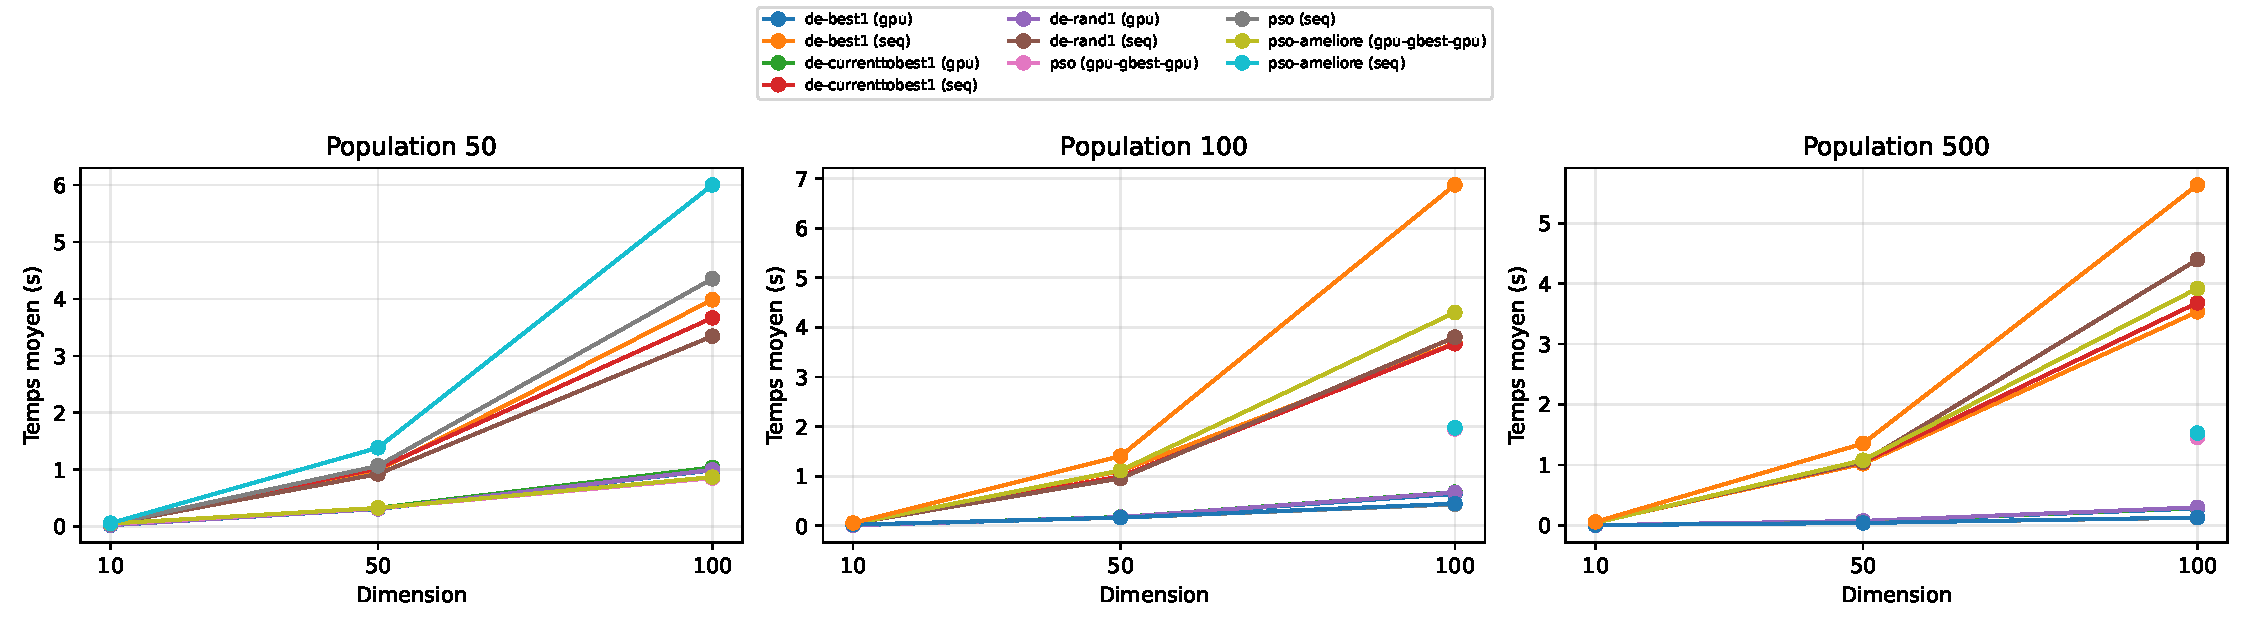
\includegraphics[width=\textwidth]{figures/runtime_vs_dimension.pdf}
\caption{Mean wall-clock time versus dimension, separated by population.}
\label{fig:generated-runtime}
\end{figure*}

\begin{figure}[t]
\centering
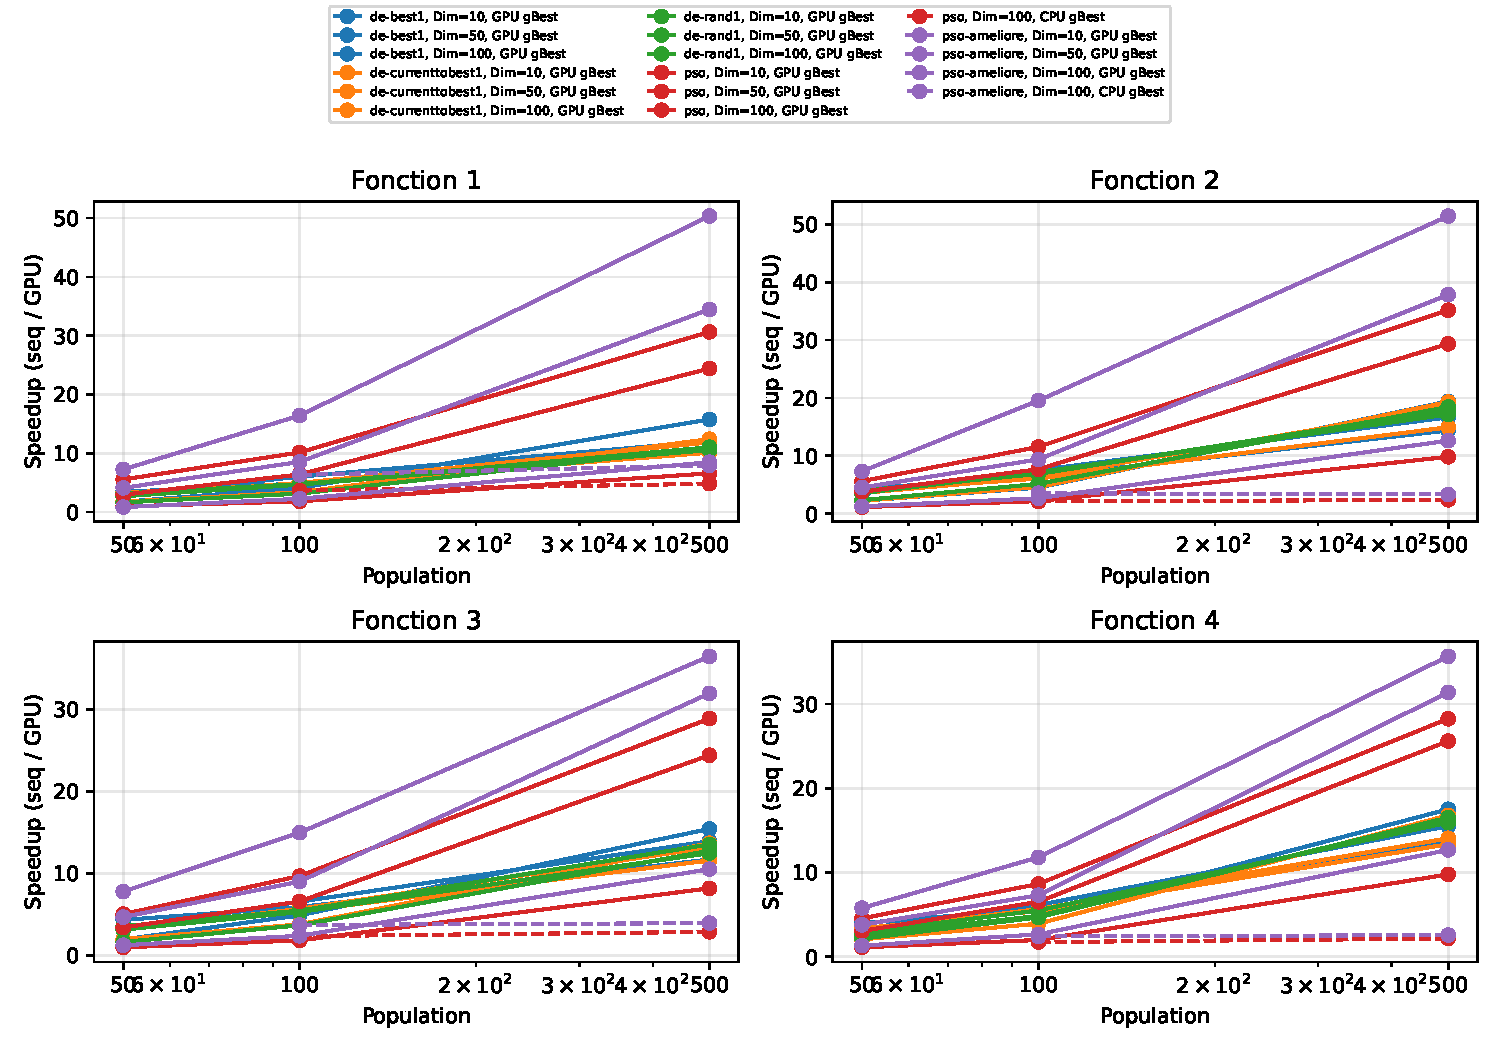
\includegraphics[width=\columnwidth]{figures/speedup_vs_population.pdf}
\caption{Measured sequential-to-GPU speedup versus population.}
\label{fig:generated-speedup}
\end{figure}

\begin{figure*}[t]
\centering
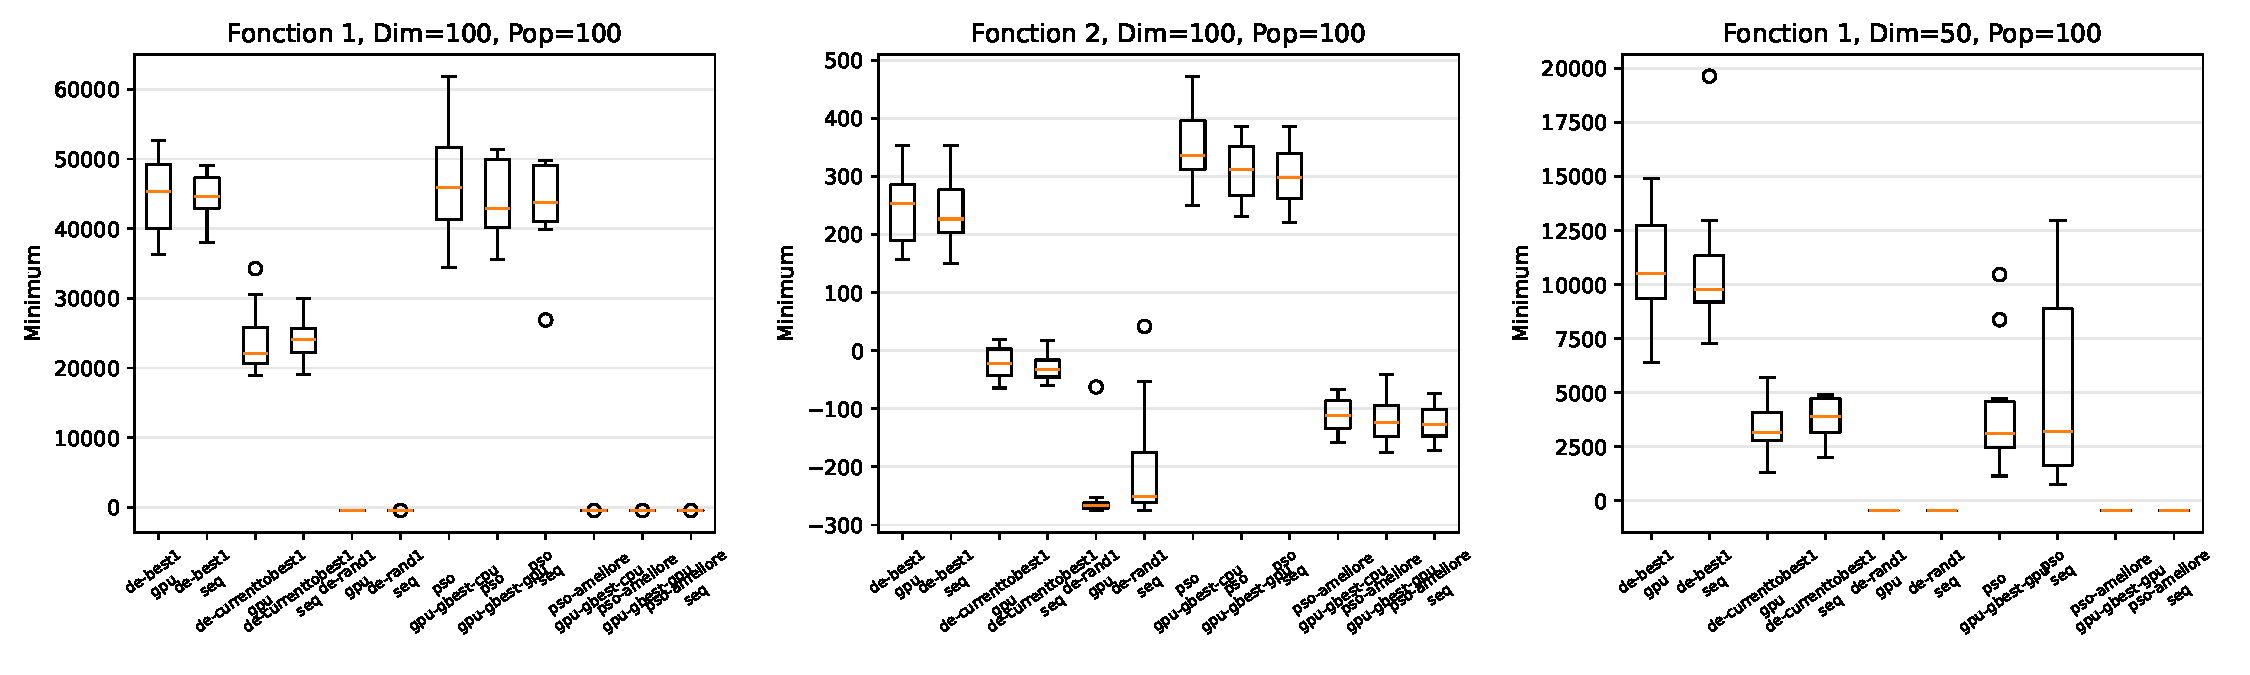
\includegraphics[width=\textwidth]{figures/minimum_boxplots.pdf}
\caption{Minimum fitness over independent runs for representative
configurations.}
\label{fig:generated-minima}
\end{figure*}

\section{Conclusion}
\label{sec:conclusion}
This paper documents a corrected sequential and CUDA PSO implementation,
four shared shifted objectives, selectable CPU/GPU global-best handling, and
a bounded-velocity variant. Preliminary results indicate that the improved
variant addresses the observed Sphere divergence at dimension 100, while
Rastrigin and Rosenbrock remain difficult at that dimension. Preliminary
timings suggest a benefit from computing the global best on the GPU, but a
complete ten-run sequential and GPU campaign has now been analyzed with the
generated tables and figures. The PSO--DE GPU comparison reports descriptive
fitness and runtime alongside the existing Mann--Whitney tests, distinguishing
significant quality differences from non-significant results. Further work
should address multiple-comparison corrections, effect sizes, and comparisons
with literature under matching benchmark and timing conditions.

\bibliographystyle{IEEEtran}
\bibliography{references}

\end{document}
